\documentclass[a4j,twocolumn,dvipdfmx]{jsarticle}

% =========================================================
% パッケージ
% =========================================================
\usepackage[
  a4paper,
  left=2.0cm,
  right=2.0cm,
  top=2.0cm,
  bottom=2.0cm
]{geometry}

\usepackage{amsmath}
\usepackage[dvipdfmx]{graphicx}
\usepackage{titlesec}
\usepackage{enumitem}
\usepackage{tikz}
\usetikzlibrary{positioning}
\usepackage{float}
\usepackage{algorithm}
\usepackage{algpseudocode}
\usepackage{booktabs}

\raggedbottom

% =========================================================
% 見出し設定
% =========================================================
\titleformat{\section}[block]
  {\normalfont\large\bfseries}
  {\thesection}{0.7em}{}

\titleformat{\subsection}[block]
  {\normalfont\normalsize\bfseries}
  {\thesubsection}{0.7em}{}

\titleformat{\subsubsection}[block]
  {\normalfont\normalsize\bfseries}
  {\thesubsubsection}{0.7em}{}

% 見出し前後の余白
\titlespacing*{\section}
  {0pt}{1.5ex plus 0.5ex minus 0.2ex}{0.8ex}

\titlespacing*{\subsection}
  {0pt}{1.2ex plus 0.4ex minus 0.2ex}{0.6ex}

% =========================================================
% 箇条書き設定
% =========================================================
\setlist[itemize]{
  topsep=3pt,
  itemsep=1pt,
  parsep=0pt,
  leftmargin=*
}

% =========================================================
% タイトル
% =========================================================
\title{\vspace{-1.5em}\textbf{実験結果}}
\author{3CDA2216 笠原秀星}
\date{\today}


\begin{document}

\maketitle

% =========================================================
\section{FedAvg（IID環境）における悪性クライアント比率別の評価}
% =========================================================


\subsection{FedAvg：IID・悪性クライアント比率 0.0}

\subsubsection{実験条件}

\begin{itemize}
    \item \textbf{Aggregation method:} FedAvg
    \item \textbf{Data split:} IID
    \item \textbf{Malicious ratio:} 0.0
    \item \textbf{Attack:} Adaptive attack
    \item \textbf{Number of rounds:} 20
    \item \textbf{Seeds:} 1, 2, 3
\end{itemize}

% =========================================================
% 実験結果表
% =========================================================

\begin{table}[H]
\centering

\caption{FedAvg（IID，悪性クライアント比率 0.0）における
Accuracy および Loss}

\label{tab:fedavg_iid_ratio0}

\footnotesize
\setlength{\tabcolsep}{2.5pt}
\renewcommand{\arraystretch}{0.90}

\resizebox{\columnwidth}{!}{%
\begin{tabular}{c cc cc cc}

\toprule

& \multicolumn{2}{c}{Seed 1}
& \multicolumn{2}{c}{Seed 2}
& \multicolumn{2}{c}{Seed 3} \\

\cmidrule(lr){2-3}
\cmidrule(lr){4-5}
\cmidrule(lr){6-7}

Round
& Acc. & Loss
& Acc. & Loss
& Acc. & Loss \\

\midrule

0  & 0.1416 & 2.2942 & 0.0975 & 2.2943 & 0.0877 & 2.3024 \\
1  & 0.7636 & 1.2828 & 0.7217 & 1.2678 & 0.7259 & 1.2749 \\
2  & 0.8531 & 0.6233 & 0.8399 & 0.6505 & 0.8336 & 0.6461 \\
3  & 0.8811 & 0.4643 & 0.8725 & 0.4871 & 0.8694 & 0.5020 \\
4  & 0.8948 & 0.3896 & 0.8869 & 0.4124 & 0.8851 & 0.4265 \\
5  & 0.9038 & 0.3488 & 0.8957 & 0.3697 & 0.8970 & 0.3782 \\
6  & 0.9081 & 0.3229 & 0.9006 & 0.3415 & 0.9037 & 0.3449 \\
7  & 0.9136 & 0.3033 & 0.9049 & 0.3221 & 0.9102 & 0.3213 \\
8  & 0.9156 & 0.2891 & 0.9096 & 0.3036 & 0.9136 & 0.3040 \\
9  & 0.9180 & 0.2761 & 0.9128 & 0.2904 & 0.9156 & 0.2909 \\
10 & 0.9206 & 0.2655 & 0.9156 & 0.2783 & 0.9182 & 0.2785 \\
11 & 0.9223 & 0.2569 & 0.9200 & 0.2674 & 0.9212 & 0.2675 \\
12 & 0.9254 & 0.2476 & 0.9214 & 0.2591 & 0.9236 & 0.2588 \\
13 & 0.9271 & 0.2409 & 0.9236 & 0.2504 & 0.9256 & 0.2504 \\
14 & 0.9283 & 0.2336 & 0.9263 & 0.2419 & 0.9286 & 0.2425 \\
15 & 0.9301 & 0.2268 & 0.9284 & 0.2351 & 0.9300 & 0.2356 \\
16 & 0.9322 & 0.2200 & 0.9299 & 0.2285 & 0.9308 & 0.2300 \\
17 & 0.9331 & 0.2138 & 0.9336 & 0.2203 & 0.9322 & 0.2229 \\
18 & 0.9355 & 0.2074 & 0.9359 & 0.2146 & 0.9339 & 0.2173 \\
19 & 0.9380 & 0.2027 & 0.9362 & 0.2090 & 0.9352 & 0.2111 \\
20 & 0.9382 & 0.1989 & 0.9383 & 0.2040 & 0.9368 & 0.2071 \\

\bottomrule

\end{tabular}%
}

\end{table}
\begin{figure}[H]
    \centering
    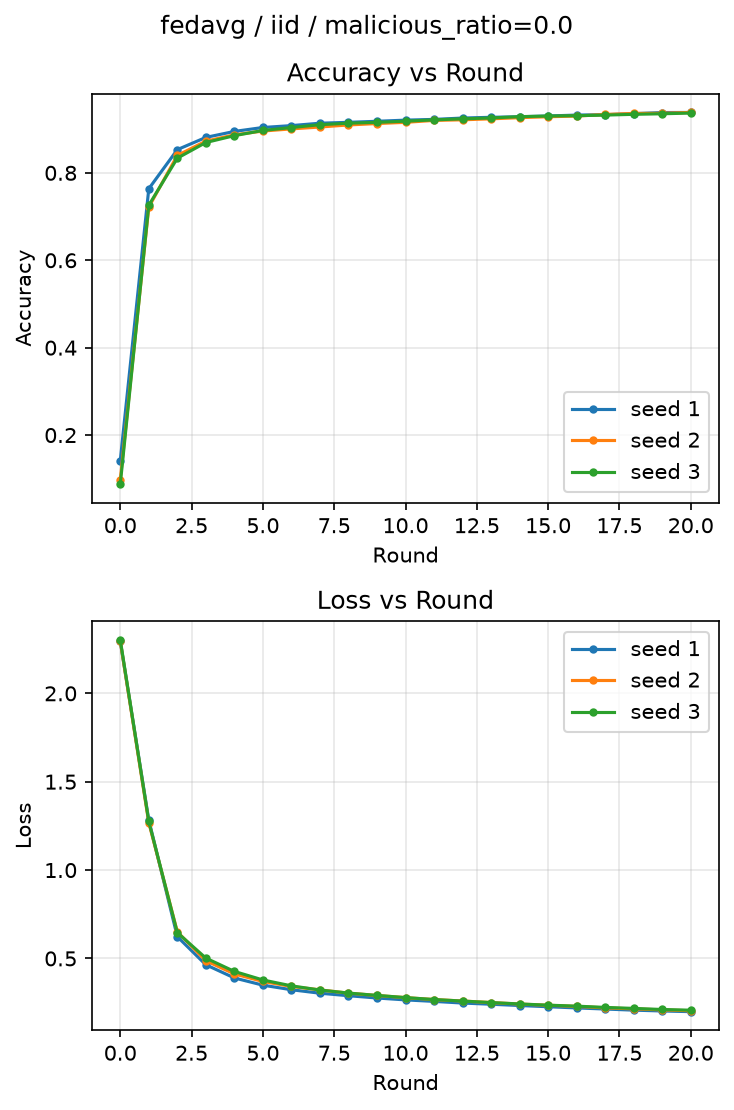
\includegraphics[width=\columnwidth]{seed_curves.png}
    \caption{Seed ごとの Round-Accuracy および Round-Loss の推移}
    \label{fig:seed_curves}
\end{figure}
% =========================================================
\subsubsection{結果}
% =========================================================

表\ref{tab:fedavg_iid_ratio0}に，各ラウンドにおける
Accuracy および Loss を示す．

学習開始時（Round 0）の Accuracy は約 0.09--0.14 であったが，
Round 1 では約 0.72--0.76 まで上昇した．
その後も学習ラウンドの進行に伴って Accuracy は継続的に向上し，
Round 20 ではすべての Seed において約 0.94 に達した．

一方，Loss は Round 0 の約 2.29--2.30 から継続的に減少し，
Round 20 では約 0.20--0.21 となった．
また，3つの Seed 間で Accuracy および Loss に大きな差は見られず，
異なる乱数シードに対しても同様の学習傾向が確認された．

\clearpage
% =========================================================
\subsection{FedAvg：IID・悪性クライアント比率 0.1}
% =========================================================

\subsubsection{実験条件}

\begin{itemize}
    \item \textbf{Aggregation method:} FedAvg
    \item \textbf{Data split:} IID
    \item \textbf{Malicious ratio:} 0.1
    \item \textbf{Attack:} Adaptive attack
    \item \textbf{Number of rounds:} 20
    \item \textbf{Seeds:} 1, 2, 3
\end{itemize}

% =========================================================
% 実験結果表
% =========================================================

\begin{table}[H]
\centering

\caption{FedAvg（IID，悪性クライアント比率 0.1）における
Accuracy および Loss}

\label{tab:fedavg_iid_ratio0.1}

\footnotesize
\setlength{\tabcolsep}{2.5pt}
\renewcommand{\arraystretch}{0.90}

\resizebox{\columnwidth}{!}{%
\begin{tabular}{c cc cc cc}

\toprule

& \multicolumn{2}{c}{Seed 1}
& \multicolumn{2}{c}{Seed 2}
& \multicolumn{2}{c}{Seed 3} \\

\cmidrule(lr){2-3}
\cmidrule(lr){4-5}
\cmidrule(lr){6-7}

Round
& Acc. & Loss
& Acc. & Loss
& Acc. & Loss \\

\midrule

0  & 0.1008 & 2.3051 & 0.0817 & 2.3042 & 0.0608 & 2.3152 \\
1  & 0.7395 & 0.8810 & 0.6801 & 0.9412 & 0.7056 & 0.9331 \\
2  & 0.8484 & 0.5087 & 0.8372 & 0.5310 & 0.8329 & 0.5351 \\
3  & 0.8869 & 0.4138 & 0.8806 & 0.4062 & 0.8808 & 0.4107 \\
4  & 0.8944 & 0.3540 & 0.8947 & 0.3543 & 0.8931 & 0.3396 \\
5  & 0.9095 & 0.3165 & 0.9112 & 0.3099 & 0.9093 & 0.3112 \\
6  & 0.9089 & 0.3013 & 0.9053 & 0.3030 & 0.9105 & 0.2889 \\
7  & 0.9205 & 0.2748 & 0.9209 & 0.2693 & 0.9126 & 0.2854 \\
8  & 0.9213 & 0.2616 & 0.9207 & 0.2593 & 0.9210 & 0.2582 \\
9  & 0.9270 & 0.2465 & 0.9251 & 0.2522 & 0.9261 & 0.2421 \\
10 & 0.9306 & 0.2371 & 0.9272 & 0.2394 & 0.9304 & 0.2305 \\
11 & 0.9289 & 0.2352 & 0.9347 & 0.2224 & 0.9352 & 0.2144 \\
12 & 0.9354 & 0.2202 & 0.9370 & 0.2110 & 0.9344 & 0.2174 \\
13 & 0.9361 & 0.2104 & 0.9411 & 0.2026 & 0.9398 & 0.1976 \\
14 & 0.9382 & 0.2047 & 0.9404 & 0.1990 & 0.9369 & 0.2061 \\
15 & 0.9368 & 0.2039 & 0.9419 & 0.1948 & 0.9419 & 0.1871 \\
16 & 0.9403 & 0.1972 & 0.9425 & 0.1871 & 0.9389 & 0.2025 \\
17 & 0.9404 & 0.1996 & 0.9439 & 0.1872 & 0.9419 & 0.1864 \\
18 & 0.9414 & 0.2013 & 0.9420 & 0.1907 & 0.9369 & 0.2140 \\
19 & 0.9346 & 0.2194 & 0.9443 & 0.1869 & 0.9381 & 0.1956 \\
20 & 0.9367 & 0.2168 & 0.9418 & 0.1920 & 0.9299 & 0.2462 \\

\bottomrule

\end{tabular}%
}

\end{table}
\begin{figure}[H]
    \centering
    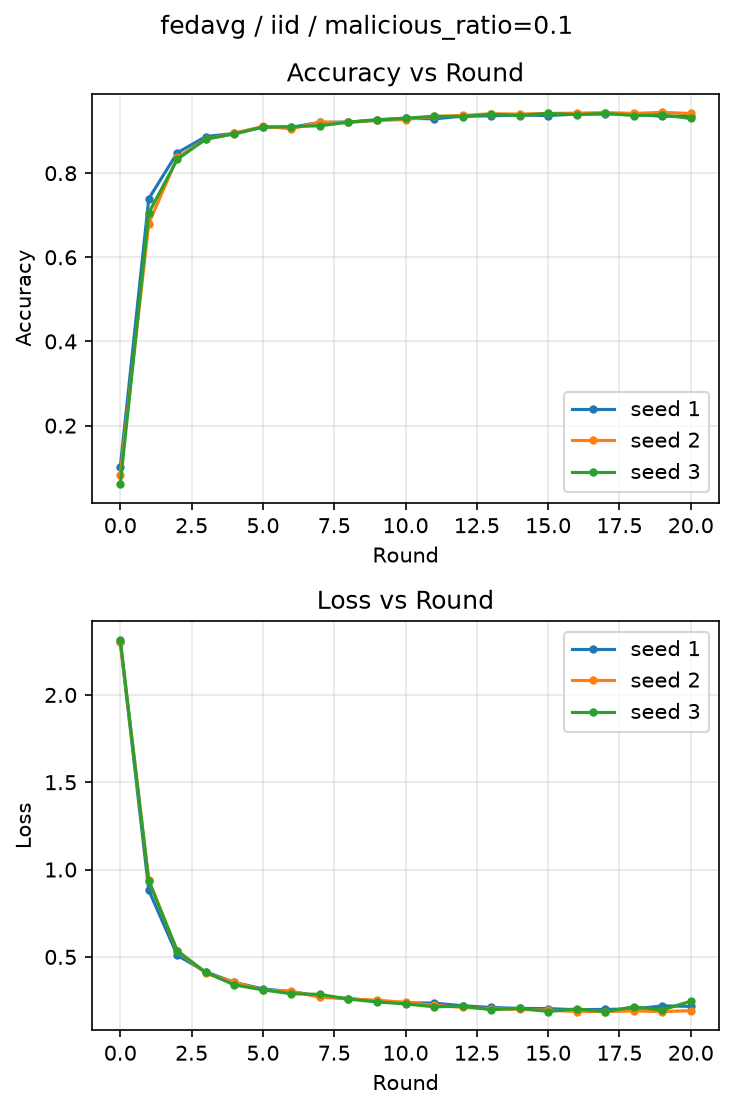
\includegraphics[width=\columnwidth]{seed_curves_ratio0.1.png}
    \caption{Seed ごとの Round-Accuracy および Round-Loss の推移（悪性クライアント比率 0.1）}
    \label{fig:seed_curves_ratio0.1}
\end{figure}
% =========================================================
\subsubsection{結果}
% =========================================================

表\ref{tab:fedavg_iid_ratio0.1}に，各ラウンドにおける
Accuracy および Loss を示す．

学習開始時（Round 0）の Accuracy は Seed によって約 0.06--0.10 とばらつきが見られたが，
Round 1 では約 0.68--0.74 まで上昇した．
その後も学習ラウンドの進行に伴って Accuracy は継続的に向上し，
Round 20 ではすべての Seed において約 0.93--0.94 に達した．

一方，Loss は Round 0 の約 2.30--2.32 から継続的に減少し，
Round 20 では約 0.19--0.25 となった．
悪性クライアント比率 0.0 の場合と比較すると，
最終的な Accuracy はほぼ同水準にとどまったものの，
Seed 3 で Round 19--20 にかけて Loss がやや増加する場面が見られた．
malicious ratio 0.1（クライアント数100中10クライアント）では，
悪性クライアントの Scale Attack による更新が単純平均に混入しても，
残り90\%の正常な更新によって希釈され，学習全体としては
悪性クライアント比率 0.0 の場合とほぼ同水準の性能を維持できたと考えられる．

\clearpage
% =========================================================
\subsection{FedAvg：IID・悪性クライアント比率 0.2}
% =========================================================

\subsubsection{実験条件}

\begin{itemize}
    \item \textbf{Aggregation method:} FedAvg
    \item \textbf{Data split:} IID
    \item \textbf{Malicious ratio:} 0.2
    \item \textbf{Attack:} Adaptive attack
    \item \textbf{Number of rounds:} 20
    \item \textbf{Seeds:} 1, 2, 3
\end{itemize}

% =========================================================
% 実験結果表
% =========================================================

\begin{table}[H]
\centering

\caption{FedAvg（IID，悪性クライアント比率 0.2）における
Accuracy および Loss}

\label{tab:fedavg_iid_ratio0.2}

\footnotesize
\setlength{\tabcolsep}{2.5pt}
\renewcommand{\arraystretch}{0.90}

\resizebox{\columnwidth}{!}{%
\begin{tabular}{c cc cc cc}

\toprule

& \multicolumn{2}{c}{Seed 1}
& \multicolumn{2}{c}{Seed 2}
& \multicolumn{2}{c}{Seed 3} \\

\cmidrule(lr){2-3}
\cmidrule(lr){4-5}
\cmidrule(lr){6-7}

Round
& Acc. & Loss
& Acc. & Loss
& Acc. & Loss \\

\midrule

0  & 0.0778 & 2.3114 & 0.0869 & 2.2993 & 0.0844 & 2.3129 \\
1  & 0.6285 & 1.2967 & 0.6540 & 1.1425 & 0.5934 & 1.3403 \\
2  & 0.5945 & 1.0478 & 0.6856 & 0.8765 & 0.5800 & 1.3043 \\
3  & 0.6020 & 1.4075 & 0.6622 & 1.0375 & 0.6616 & 1.1254 \\
4  & 0.2978 & 4.8879 & 0.5780 & 1.9192 & 0.3567 & 4.1239 \\
5  & 0.3474 & 4.0723 & 0.2637 & 5.5046 & 0.4327 & 3.6166 \\
6  & 0.3068 & 3.8003 & 0.4028 & 5.4084 & 0.3408 & 2.7942 \\
7  & 0.4908 & 3.1571 & 0.3910 & 3.8948 & 0.4221 & 4.8563 \\
8  & 0.2649 & 5.8880 & 0.3611 & 2.6517 & 0.2987 & 8.1121 \\
9  & 0.2661 & 10.8871 & 0.4259 & 3.3033 & 0.4264 & 5.5301 \\
10 & 0.4560 & 5.0990 & 0.4990 & 3.8053 & 0.4844 & 4.8675 \\
11 & 0.3958 & 5.1416 & 0.5100 & 1.6177 & 0.5771 & 2.6495 \\
12 & 0.6644 & 2.4425 & 0.5892 & 2.0458 & 0.4898 & 2.6568 \\
13 & 0.6441 & 1.3076 & 0.5014 & 3.6747 & 0.4291 & 3.6676 \\
14 & 0.6269 & 2.1362 & 0.5885 & 1.9194 & 0.4700 & 3.1586 \\
15 & 0.3989 & 4.6093 & 0.5156 & 2.7631 & 0.5194 & 3.6085 \\
16 & 0.4244 & 4.0273 & 0.5385 & 3.1985 & 0.6054 & 2.3273 \\
17 & 0.5916 & 1.8398 & 0.5363 & 3.2618 & 0.5940 & 1.9801 \\
18 & 0.6079 & 2.0978 & 0.3399 & 5.3854 & 0.6257 & 1.9355 \\
19 & 0.6875 & 2.0099 & 0.5631 & 4.8583 & 0.5236 & 3.0180 \\
20 & 0.5231 & 3.5254 & 0.4904 & 3.4841 & 0.6422 & 1.5237 \\

\bottomrule

\end{tabular}%
}

\end{table}
\begin{figure}[H]
    \centering
    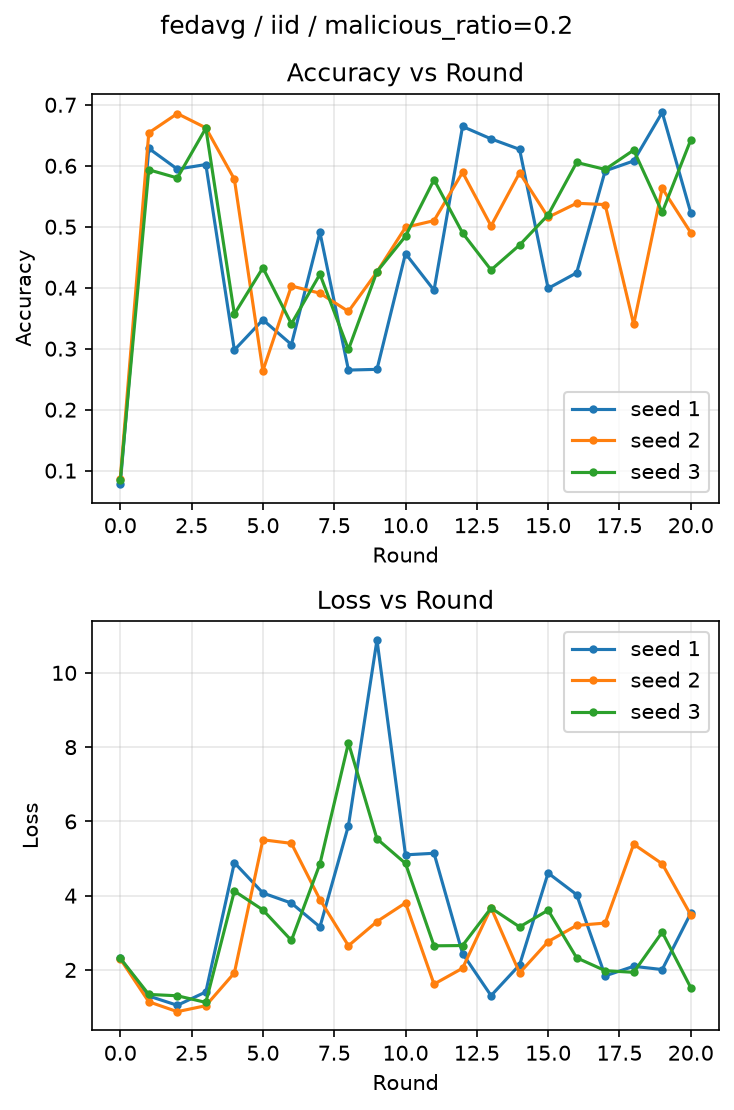
\includegraphics[width=\columnwidth]{seed_curves_ratio0.2.png}
    \caption{Seed ごとの Round-Accuracy および Round-Loss の推移（悪性クライアント比率 0.2）}
    \label{fig:seed_curves_ratio0.2}
\end{figure}
% =========================================================
\subsubsection{結果}
% =========================================================

表\ref{tab:fedavg_iid_ratio0.2}に，各ラウンドにおける
Accuracy および Loss を示す．

学習開始時（Round 0）の Accuracy は Seed によって約 0.08--0.09 とばらつきが見られ，
Round 1 では約 0.59--0.65 まで上昇した．
しかし，悪性クライアント比率 0.0，0.1 の場合とは異なり，
Round 2 以降 Accuracy は単調に向上せず，約 0.26--0.69 の範囲で
ラウンドごとに大きく上下する不安定な挙動を示した．
Loss についても Round 9（Seed 1）で最大 10.8871 に達するなど，
学習全体を通じて大きなスパイクが繰り返し観測された．
Round 20 時点の Accuracy は約 0.49--0.64，Loss は約 1.52--3.53 であり，
悪性クライアント比率 0.0 の場合（最終 Accuracy 平均 約 0.94）と比較して
大幅に低下した．

FedAvg は集約時に外れ値を除外する仕組みを持たないため，
悪性クライアントが送信する Scale Attack（真の更新量を10倍に拡大した
悪性更新）がそのまま単純平均に混入し，グローバルモデルを毎ラウンド
大きく振動させたと考えられる．悪性クライアント比率 0.1 では
希釈効果（100クライアント中10クライアントの影響が90\%の正常な
更新によって緩和される）によって性能が維持されていたのに対し，
悪性クライアント比率 0.2 ではこの希釈効果だけでは攻撃の影響を
吸収しきれなくなったことが示唆される．

\clearpage
% =========================================================
\subsection{FedAvg：IID・悪性クライアント比率 0.3}
% =========================================================

\subsubsection{実験条件}

\begin{itemize}
    \item \textbf{Aggregation method:} FedAvg
    \item \textbf{Data split:} IID
    \item \textbf{Malicious ratio:} 0.3
    \item \textbf{Attack:} Adaptive attack
    \item \textbf{Number of rounds:} 20
    \item \textbf{Seeds:} 1, 2, 3
\end{itemize}

% =========================================================
% 実験結果表
% =========================================================

\begin{table}[H]
\centering

\caption{FedAvg（IID，悪性クライアント比率 0.3）における
Accuracy および Loss}

\label{tab:fedavg_iid_ratio0.3}

\footnotesize
\setlength{\tabcolsep}{2.5pt}
\renewcommand{\arraystretch}{0.90}

\resizebox{\columnwidth}{!}{%
\begin{tabular}{c cc cc cc}

\toprule

& \multicolumn{2}{c}{Seed 1}
& \multicolumn{2}{c}{Seed 2}
& \multicolumn{2}{c}{Seed 3} \\

\cmidrule(lr){2-3}
\cmidrule(lr){4-5}
\cmidrule(lr){6-7}

Round
& Acc. & Loss
& Acc. & Loss
& Acc. & Loss \\

\midrule

0  & 0.1050 & 2.3052 & 0.0871 & 2.3058 & 0.1121 & 2.3028 \\
1  & 0.4669 & 2.4719 & 0.6494 & 2.0048 & 0.6388 & 1.6048 \\
2  & 0.4176 & 5.5211 & 0.1258 & 7.9264 & 0.3630 & 3.5062 \\
3  & 0.2155 & 16.0470 & 0.2638 & 11.3932 & 0.2382 & 9.7461 \\
4  & 0.1950 & 9.2702 & 0.1685 & 9.0113 & 0.0982 & 17.7718 \\
5  & 0.3092 & 2.0615 & 0.2908 & 4.2999 & 0.1831 & 12.4552 \\
6  & 0.4707 & 3.5233 & 0.3120 & 4.1903 & 0.0986 & 12.0350 \\
7  & 0.2986 & 6.2982 & 0.3903 & 3.1011 & 0.4063 & 7.4052 \\
8  & 0.3447 & 8.0512 & 0.2819 & 5.5339 & 0.3436 & 5.2857 \\
9  & 0.3933 & 7.0966 & 0.4275 & 2.8813 & 0.4488 & 3.4722 \\
10 & 0.5659 & 1.5118 & 0.3882 & 5.0619 & 0.2295 & 6.4546 \\
11 & 0.3522 & 5.3616 & 0.4414 & 3.9600 & 0.4053 & 4.2804 \\
12 & 0.4672 & 5.4911 & 0.5925 & 1.6918 & 0.3749 & 4.3466 \\
13 & 0.5873 & 2.3319 & 0.4998 & 2.7261 & 0.5469 & 3.3843 \\
14 & 0.4728 & 2.9704 & 0.4132 & 4.2478 & 0.5318 & 2.5925 \\
15 & 0.4600 & 2.3754 & 0.4168 & 6.8800 & 0.3739 & 4.1574 \\
16 & 0.6398 & 2.2465 & 0.4692 & 2.6400 & 0.5030 & 4.6876 \\
17 & 0.5357 & 2.4792 & 0.2809 & 5.1705 & 0.5539 & 2.4600 \\
18 & 0.5437 & 3.8618 & 0.4397 & 3.6397 & 0.5016 & 3.6686 \\
19 & 0.4995 & 3.6105 & 0.4574 & 6.9452 & 0.6246 & 2.2948 \\
20 & 0.6567 & 1.8212 & 0.5257 & 6.6401 & 0.5313 & 2.3416 \\

\bottomrule

\end{tabular}%
}

\end{table}
\begin{figure}[H]
    \centering
    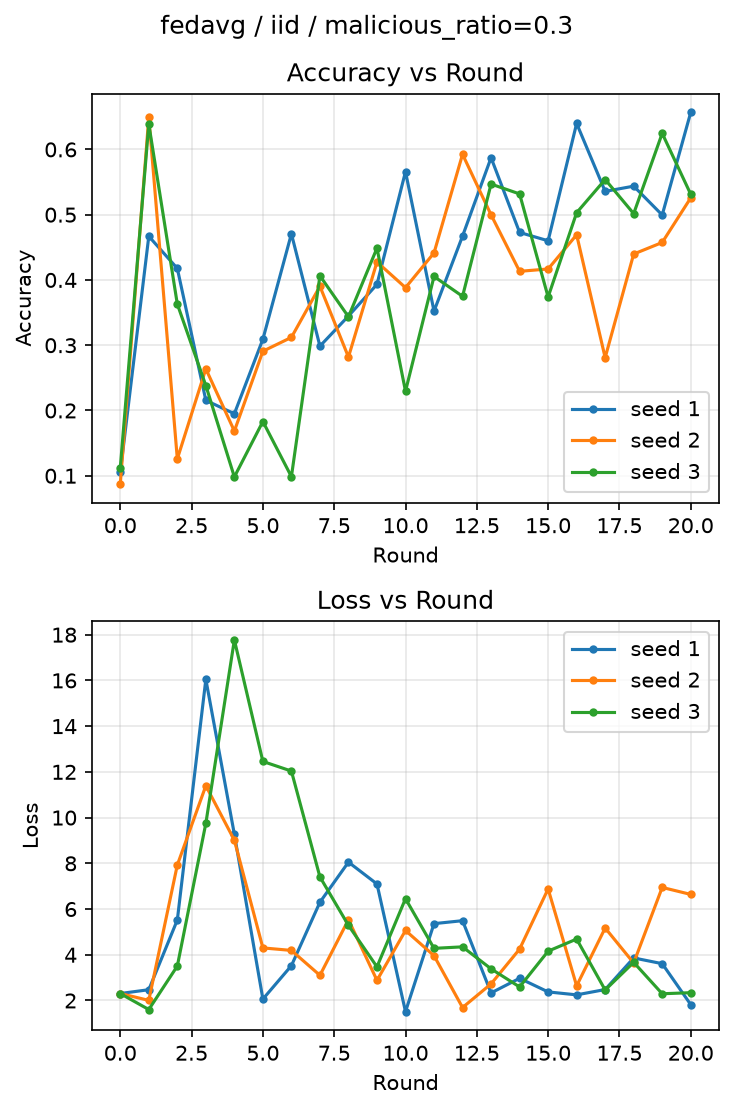
\includegraphics[width=\columnwidth]{seed_curves_ratio0.3.png}
    \caption{Seed ごとの Round-Accuracy および Round-Loss の推移（悪性クライアント比率 0.3）}
    \label{fig:seed_curves_ratio0.3}
\end{figure}
% =========================================================
\subsubsection{結果}
% =========================================================

表\ref{tab:fedavg_iid_ratio0.3}に，各ラウンドにおける
Accuracy および Loss を示す．

学習開始時（Round 0）の Accuracy は Seed によって約 0.09--0.11 とばらつきが見られ，
Round 1 では約 0.47--0.65 まで上昇した．
しかし，悪性クライアント比率 0.2 の場合よりもさらに不安定な挙動を示し，
Round 3（Seed 1）で Loss が最大 16.0470 に達するなど，
学習全体を通じて Accuracy・Loss ともに大きな振動が続いた．
Round 20 時点の Accuracy は約 0.53--0.66，Loss は約 1.82--6.64 であり，
収束したとは言い難い状態であった．

悪性クライアント数が20クライアント（比率0.2）から30クライアント
（比率0.3）へ増加したことで，Scale Attack を受けた更新が単純平均に
より多く混入するようになり，悪性クライアント比率 0.2 の場合よりも
グローバルモデルの不安定性がさらに増したと考えられる．
Seed 2 では Round 19 に Loss が 6.9452 まで悪化するなど，
Seed 間で収束の度合いにもばらつきが見られた．

\clearpage
% =========================================================
\subsection{FedAvg：IID・悪性クライアント比率別の比較（Seed 1）}
% =========================================================

\subsubsection{実験条件}

\begin{itemize}
    \item \textbf{Aggregation method:} FedAvg
    \item \textbf{Data split:} IID
    \item \textbf{Malicious ratio:} 0.0, 0.1, 0.2, 0.3
    \item \textbf{Attack:} Adaptive attack
    \item \textbf{Number of rounds:} 20
    \item \textbf{Seed:} 1
\end{itemize}

1.1--1.4 節で示した Seed 1 の結果を malicious ratio 別に
1つの図上で比較できるよう再構成した．
図の作成には \verb|result/plot_fedavg_iid_seed1_by_ratio.py| を用い，
\verb|result/results.csv| から FedAvg・IID・seed=1 の条件に一致する
run を malicious ratio ごとに抽出して描画した．

% =========================================================
% 実験結果図
% =========================================================

\begin{figure}[H]
    \centering
    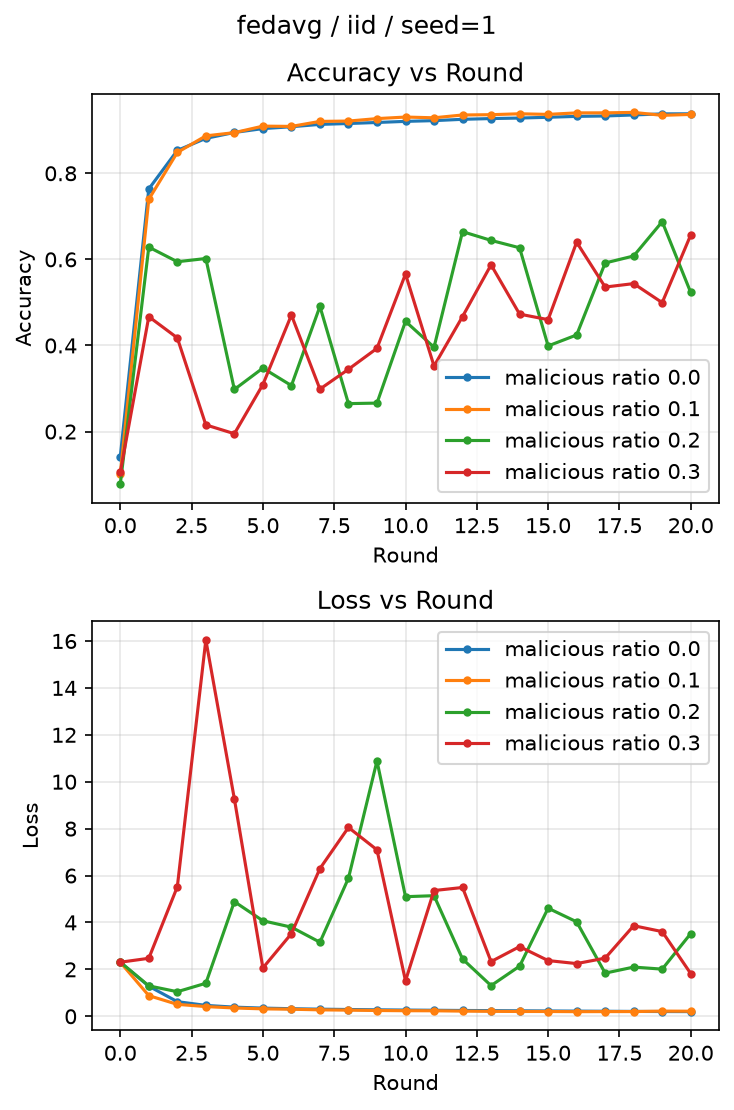
\includegraphics[width=\columnwidth]{fedavg_iid_seed1_by_ratio.png}
    \caption{FedAvg・IID・Seed 1 における malicious ratio 別の
    Round-Accuracy および Round-Loss の推移}
    \label{fig:fedavg_iid_seed1_by_ratio}
\end{figure}

% =========================================================
\subsubsection{結果}
% =========================================================

図\ref{fig:fedavg_iid_seed1_by_ratio}に，malicious ratio
0.0, 0.1, 0.2, 0.3 における Round-Accuracy および Round-Loss の推移を示す．

malicious ratio 0.0, 0.1 では Accuracy は Round 1 で急速に上昇した後
Round 20 にかけて滑らかに向上し，最終的に約 0.94 に収束した．
一方，malicious ratio 0.2, 0.3 では Round 2 以降 Accuracy が
単調に向上せず，Round 20 まで大きく上下する不安定な挙動が続いた．
Round 20 時点の Accuracy（Seed 1）は malicious ratio 0.2 で 0.5231，
malicious ratio 0.3 で 0.6567 であり，malicious ratio 0.0, 0.1 の
約 0.94 と比較して大幅に低い水準にとどまった．
Loss についても malicious ratio 0.2, 0.3 では Round 3--9 付近で
繰り返し急激なスパイク（最大 16.05）が見られ，malicious ratio 0.0,
0.1 のように単調に減少する傾向は確認できなかった．

以上より，IID 環境かつ Seed 1 において，
FedAvg は malicious ratio 0.1 までは希釈効果によって
安定した学習性能を維持できるものの，malicious ratio 0.2 以上では
Scale Attack を受けた悪性更新が単純平均に大きく混入し，
学習が不安定化・大幅な性能低下を招くことが確認された．
防御機構を持たない FedAvg は，外れ値を除外する仕組みが無いため，
悪性クライアントの割合が一定の水準を超えると Adaptive attack に
対して脆弱になることが示唆される．

\clearpage
% =========================================================
\section{FedAvg（Non-IID環境）における悪性クライアント比率別の評価}
% =========================================================

\subsection{FedAvg：Non-IID・悪性クライアント比率 0.0}

\subsubsection{実験条件}

\begin{itemize}
    \item \textbf{Aggregation method:} FedAvg
    \item \textbf{Data split:} Non-IID
    \item \textbf{Malicious ratio:} 0.0
    \item \textbf{Attack:} Adaptive attack
    \item \textbf{Number of rounds:} 20
    \item \textbf{Seeds:} 1, 2, 3
\end{itemize}

% =========================================================
% 実験結果表
% =========================================================

\begin{table}[H]
\centering

\caption{FedAvg（Non-IID，悪性クライアント比率 0.0）における
Accuracy および Loss}

\label{tab:fedavg_noniid_ratio0.0}

\footnotesize
\setlength{\tabcolsep}{2.5pt}
\renewcommand{\arraystretch}{0.90}

\resizebox{\columnwidth}{!}{%
\begin{tabular}{c cc cc cc}

\toprule

& \multicolumn{2}{c}{Seed 1}
& \multicolumn{2}{c}{Seed 2}
& \multicolumn{2}{c}{Seed 3} \\

\cmidrule(lr){2-3}
\cmidrule(lr){4-5}
\cmidrule(lr){6-7}

Round
& Acc. & Loss
& Acc. & Loss
& Acc. & Loss \\

\midrule

0  & 0.1309 & 2.3044 & 0.0551 & 2.3235 & 0.0757 & 2.3088 \\
1  & 0.6813 & 1.5418 & 0.7461 & 1.5430 & 0.6530 & 1.6055 \\
2  & 0.8172 & 0.8180 & 0.8381 & 0.7929 & 0.8122 & 0.8387 \\
3  & 0.8601 & 0.5698 & 0.8711 & 0.5429 & 0.8674 & 0.5688 \\
4  & 0.8831 & 0.4568 & 0.8886 & 0.4391 & 0.8829 & 0.4576 \\
5  & 0.8934 & 0.3930 & 0.8964 & 0.3878 & 0.8920 & 0.3995 \\
6  & 0.9004 & 0.3579 & 0.9023 & 0.3531 & 0.9016 & 0.3617 \\
7  & 0.9065 & 0.3314 & 0.9064 & 0.3291 & 0.9054 & 0.3395 \\
8  & 0.9081 & 0.3153 & 0.9097 & 0.3114 & 0.9076 & 0.3201 \\
9  & 0.9125 & 0.3000 & 0.9144 & 0.2957 & 0.9109 & 0.3065 \\
10 & 0.9146 & 0.2872 & 0.9153 & 0.2870 & 0.9140 & 0.2953 \\
11 & 0.9182 & 0.2766 & 0.9200 & 0.2753 & 0.9171 & 0.2837 \\
12 & 0.9182 & 0.2678 & 0.9224 & 0.2651 & 0.9186 & 0.2739 \\
13 & 0.9220 & 0.2597 & 0.9244 & 0.2567 & 0.9209 & 0.2656 \\
14 & 0.9251 & 0.2506 & 0.9252 & 0.2489 & 0.9238 & 0.2572 \\
15 & 0.9263 & 0.2451 & 0.9283 & 0.2420 & 0.9253 & 0.2503 \\
16 & 0.9282 & 0.2379 & 0.9302 & 0.2340 & 0.9262 & 0.2434 \\
17 & 0.9301 & 0.2300 & 0.9321 & 0.2270 & 0.9290 & 0.2357 \\
18 & 0.9322 & 0.2245 & 0.9324 & 0.2218 & 0.9303 & 0.2284 \\
19 & 0.9344 & 0.2186 & 0.9339 & 0.2151 & 0.9318 & 0.2232 \\
20 & 0.9358 & 0.2139 & 0.9360 & 0.2101 & 0.9329 & 0.2178 \\

\bottomrule

\end{tabular}%
}

\end{table}
\begin{figure}[H]
    \centering
    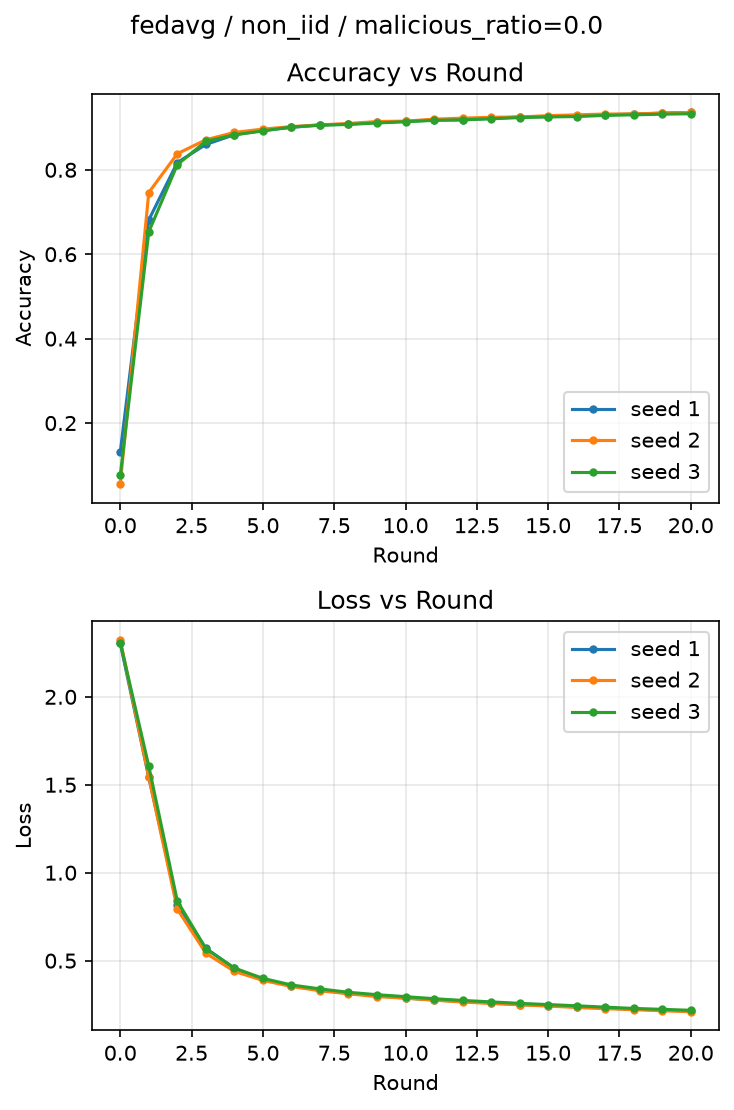
\includegraphics[width=\columnwidth]{seed_curves_noniid_ratio0.0.png}
    \caption{Seed ごとの Round-Accuracy および Round-Loss の推移（Non-IID，悪性クライアント比率 0.0）}
    \label{fig:seed_curves_noniid_ratio0.0}
\end{figure}
% =========================================================
\subsubsection{結果}
% =========================================================

表\ref{tab:fedavg_noniid_ratio0.0}に，各ラウンドにおける
Accuracy および Loss を示す．

学習開始時（Round 0）の Accuracy は約 0.06--0.13 であったが，
Round 1 では約 0.65--0.75 まで上昇した．
その後も学習ラウンドの進行に伴って Accuracy は継続的に向上し，
Round 20 ではすべての Seed において約 0.93 に達した．

一方，Loss は Round 0 の約 2.30--2.32 から継続的に減少し，
Round 20 では約 0.21--0.22 となった．
IID 環境の場合（表\ref{tab:fedavg_iid_ratio0}）と比較すると，
学習全体の収束傾向および最終的な Accuracy・Loss の水準はほぼ同等であり，
malicious ratio 0.0（悪性クライアントなし）では
Non-IID なデータ分布による大きな影響は見られなかった．

\clearpage
% =========================================================
\subsection{FedAvg：Non-IID・悪性クライアント比率 0.1}
% =========================================================

\subsubsection{実験条件}

\begin{itemize}
    \item \textbf{Aggregation method:} FedAvg
    \item \textbf{Data split:} Non-IID
    \item \textbf{Malicious ratio:} 0.1
    \item \textbf{Attack:} Adaptive attack
    \item \textbf{Number of rounds:} 20
    \item \textbf{Seeds:} 1, 2, 3
\end{itemize}

% =========================================================
% 実験結果表
% =========================================================

\begin{table}[H]
\centering

\caption{FedAvg（Non-IID，悪性クライアント比率 0.1）における
Accuracy および Loss}

\label{tab:fedavg_noniid_ratio0.1}

\footnotesize
\setlength{\tabcolsep}{2.5pt}
\renewcommand{\arraystretch}{0.90}

\resizebox{\columnwidth}{!}{%
\begin{tabular}{c cc cc cc}

\toprule

& \multicolumn{2}{c}{Seed 1}
& \multicolumn{2}{c}{Seed 2}
& \multicolumn{2}{c}{Seed 3} \\

\cmidrule(lr){2-3}
\cmidrule(lr){4-5}
\cmidrule(lr){6-7}

Round
& Acc. & Loss
& Acc. & Loss
& Acc. & Loss \\

\midrule

0  & 0.0888 & 2.3117 & 0.0956 & 2.3107 & 0.1141 & 2.2973 \\
1  & 0.4907 & 1.4176 & 0.5263 & 1.3088 & 0.5860 & 1.3126 \\
2  & 0.7903 & 0.6440 & 0.7408 & 0.7405 & 0.8314 & 0.5615 \\
3  & 0.8068 & 0.6132 & 0.7298 & 0.7646 & 0.8135 & 0.5911 \\
4  & 0.8762 & 0.4067 & 0.7494 & 0.6993 & 0.8856 & 0.3946 \\
5  & 0.8532 & 0.4731 & 0.7250 & 0.8406 & 0.8468 & 0.5037 \\
6  & 0.8952 & 0.3309 & 0.6832 & 0.9045 & 0.8963 & 0.3408 \\
7  & 0.8750 & 0.4112 & 0.7147 & 0.9640 & 0.8494 & 0.4967 \\
8  & 0.9118 & 0.2813 & 0.6961 & 0.8878 & 0.8941 & 0.3333 \\
9  & 0.9073 & 0.3085 & 0.7339 & 0.9507 & 0.8517 & 0.5064 \\
10 & 0.9232 & 0.2505 & 0.7600 & 0.7094 & 0.8898 & 0.3373 \\
11 & 0.9226 & 0.2639 & 0.7862 & 0.7605 & 0.8440 & 0.5517 \\
12 & 0.9278 & 0.2372 & 0.7814 & 0.6721 & 0.8879 & 0.3355 \\
13 & 0.9266 & 0.2440 & 0.7987 & 0.7292 & 0.8483 & 0.5222 \\
14 & 0.9345 & 0.2156 & 0.7965 & 0.6483 & 0.8893 & 0.3314 \\
15 & 0.9338 & 0.2176 & 0.7889 & 0.7851 & 0.8475 & 0.5202 \\
16 & 0.9370 & 0.2101 & 0.7992 & 0.6833 & 0.8794 & 0.3563 \\
17 & 0.9369 & 0.2048 & 0.7883 & 0.7947 & 0.8448 & 0.5332 \\
18 & 0.9368 & 0.2045 & 0.7898 & 0.7746 & 0.8722 & 0.3961 \\
19 & 0.9404 & 0.1903 & 0.8333 & 0.6385 & 0.8187 & 0.6207 \\
20 & 0.9407 & 0.1938 & 0.8391 & 0.6121 & 0.8574 & 0.4563 \\

\bottomrule

\end{tabular}%
}

\end{table}
\begin{figure}[H]
    \centering
    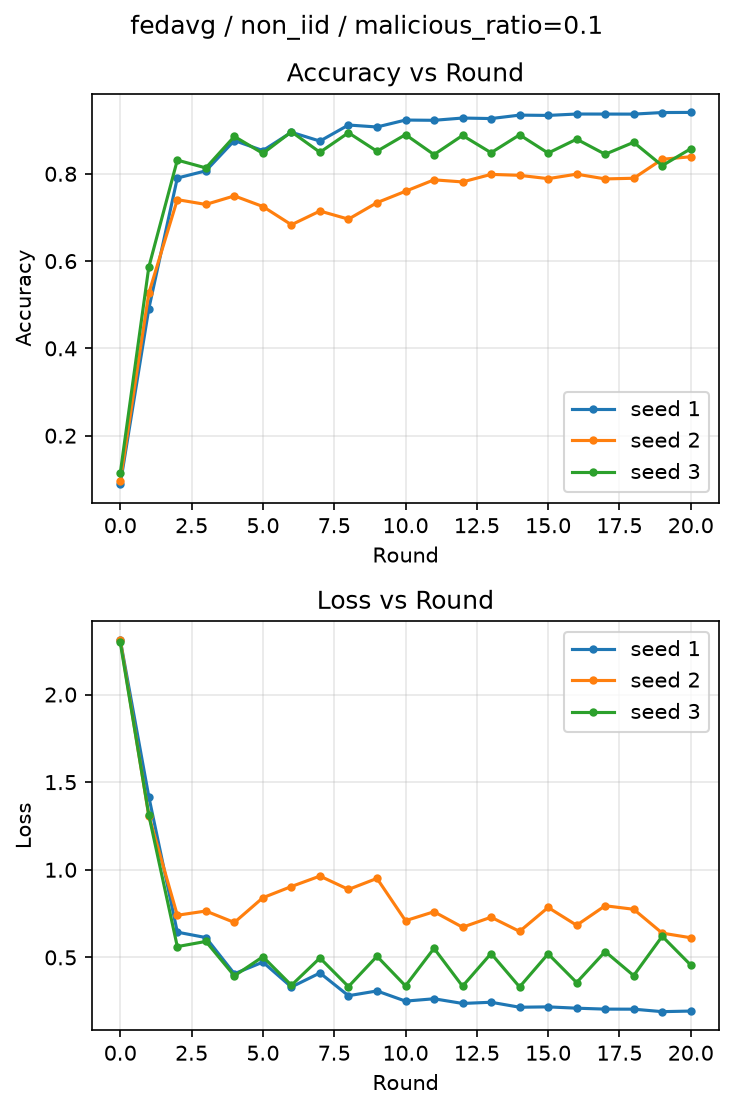
\includegraphics[width=\columnwidth]{seed_curves_noniid_ratio0.1.png}
    \caption{Seed ごとの Round-Accuracy および Round-Loss の推移（Non-IID，悪性クライアント比率 0.1）}
    \label{fig:seed_curves_noniid_ratio0.1}
\end{figure}
% =========================================================
\subsubsection{結果}
% =========================================================

表\ref{tab:fedavg_noniid_ratio0.1}に，各ラウンドにおける
Accuracy および Loss を示す．

学習開始時（Round 0）の Accuracy は Seed によって約 0.09--0.11 とばらつきが見られ，
Round 1 では約 0.49--0.59 まで上昇した．
Seed 1・Seed 3 ではその後も Accuracy が順調に向上し，
Round 20 時点でそれぞれ約 0.9407，0.8574 に達した．
一方 Seed 2 のみ Round 6 付近から約 0.68--0.80 の水準で頭打ちとなり，
Round 20 時点でも約 0.8391 にとどまった．
Loss についても Seed 2 は Round 20 時点で約 0.6121 と，
Seed 1（約 0.1938）・Seed 3（約 0.4563）より高い水準で推移した．

Non-IID 環境ではクライアントごとの保有ラベルが偏っているため，
Scale Attack を受けた悪性クライアントの更新が集約結果に与える影響が
Seed（すなわちデータ分割や悪性クライアントの選出）によって
異なる形で現れ，Seed 2 のみ学習が不安定化したと考えられる．

\clearpage
% =========================================================
\subsection{FedAvg：Non-IID・悪性クライアント比率 0.2}
% =========================================================

\subsubsection{実験条件}

\begin{itemize}
    \item \textbf{Aggregation method:} FedAvg
    \item \textbf{Data split:} Non-IID
    \item \textbf{Malicious ratio:} 0.2
    \item \textbf{Attack:} Adaptive attack
    \item \textbf{Number of rounds:} 20
    \item \textbf{Seeds:} 1, 2, 3
\end{itemize}

% =========================================================
% 実験結果表
% =========================================================

\begin{table}[H]
\centering

\caption{FedAvg（Non-IID，悪性クライアント比率 0.2）における
Accuracy および Loss}

\label{tab:fedavg_noniid_ratio0.2}

\footnotesize
\setlength{\tabcolsep}{2.5pt}
\renewcommand{\arraystretch}{0.90}

\resizebox{\columnwidth}{!}{%
\begin{tabular}{c cc cc cc}

\toprule

& \multicolumn{2}{c}{Seed 1}
& \multicolumn{2}{c}{Seed 2}
& \multicolumn{2}{c}{Seed 3} \\

\cmidrule(lr){2-3}
\cmidrule(lr){4-5}
\cmidrule(lr){6-7}

Round
& Acc. & Loss
& Acc. & Loss
& Acc. & Loss \\

\midrule

0  & 0.0973 & 2.3204 & 0.0638 & 2.3094 & 0.0991 & 2.3226 \\
1  & 0.5410 & 1.5413 & 0.4984 & 1.6995 & 0.5714 & 1.2292 \\
2  & 0.5934 & 1.3894 & 0.6984 & 1.0449 & 0.6353 & 1.1932 \\
3  & 0.5378 & 2.5099 & 0.4184 & 2.4602 & 0.4155 & 2.6081 \\
4  & 0.2775 & 3.6061 & 0.4709 & 2.4167 & 0.3382 & 3.5149 \\
5  & 0.5220 & 2.6530 & 0.2893 & 4.9162 & 0.2979 & 2.6513 \\
6  & 0.3476 & 1.9810 & 0.4977 & 2.2910 & 0.5951 & 2.1735 \\
7  & 0.5902 & 2.4553 & 0.3096 & 3.7268 & 0.1992 & 6.5454 \\
8  & 0.3308 & 3.0394 & 0.3922 & 4.0428 & 0.5332 & 4.3001 \\
9  & 0.5940 & 2.4173 & 0.4561 & 2.9964 & 0.5326 & 2.3781 \\
10 & 0.5829 & 1.7733 & 0.6216 & 1.3719 & 0.4945 & 3.6104 \\
11 & 0.5622 & 2.6095 & 0.5309 & 2.7498 & 0.4640 & 3.1000 \\
12 & 0.6217 & 2.6759 & 0.5416 & 2.2559 & 0.4951 & 2.3435 \\
13 & 0.6387 & 1.8780 & 0.5389 & 2.6607 & 0.4315 & 4.7904 \\
14 & 0.5614 & 2.2875 & 0.5124 & 2.2549 & 0.6290 & 2.4926 \\
15 & 0.5870 & 2.6185 & 0.5629 & 2.6167 & 0.5226 & 1.9718 \\
16 & 0.6694 & 1.3393 & 0.6023 & 1.6619 & 0.6477 & 1.5631 \\
17 & 0.5571 & 2.2798 & 0.5506 & 2.4055 & 0.6615 & 1.5053 \\
18 & 0.7287 & 1.5247 & 0.6948 & 1.5097 & 0.6122 & 1.8498 \\
19 & 0.5659 & 2.4085 & 0.6261 & 1.5921 & 0.6393 & 2.5925 \\
20 & 0.7097 & 1.5180 & 0.7113 & 1.3562 & 0.6039 & 1.7788 \\

\bottomrule

\end{tabular}%
}

\end{table}
\begin{figure}[H]
    \centering
    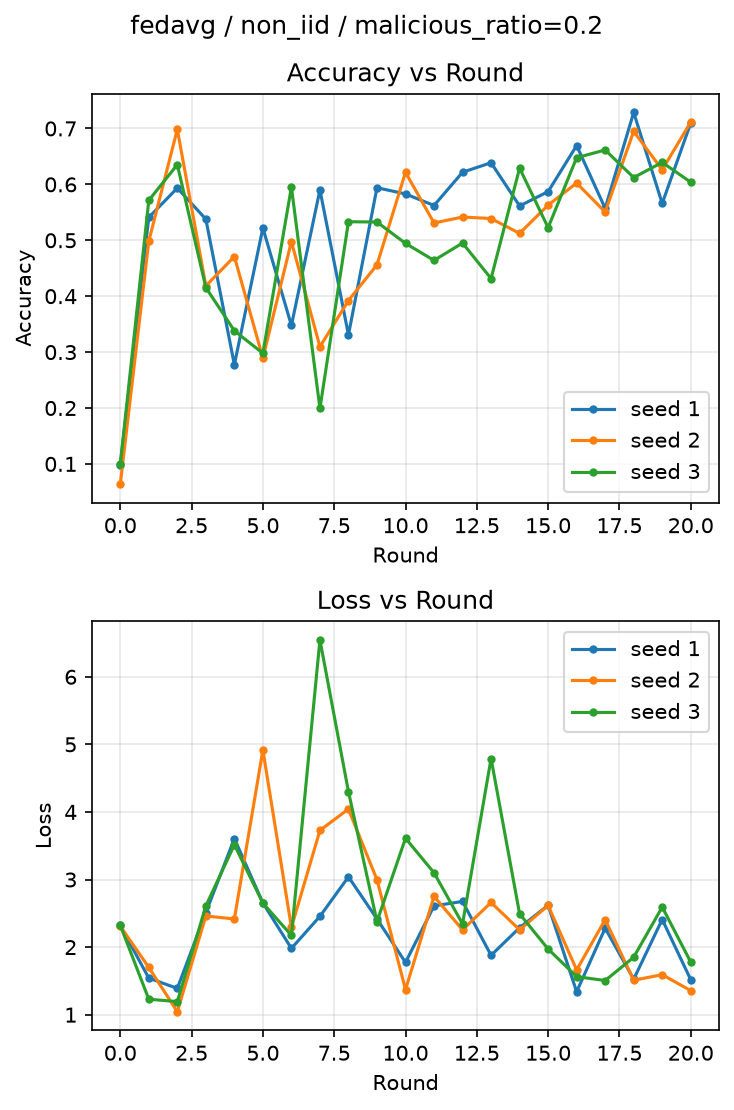
\includegraphics[width=\columnwidth]{seed_curves_noniid_ratio0.2.png}
    \caption{Seed ごとの Round-Accuracy および Round-Loss の推移（Non-IID，悪性クライアント比率 0.2）}
    \label{fig:seed_curves_noniid_ratio0.2}
\end{figure}
% =========================================================
\subsubsection{結果}
% =========================================================

表\ref{tab:fedavg_noniid_ratio0.2}に，各ラウンドにおける
Accuracy および Loss を示す．

学習開始時（Round 0）の Accuracy は Seed によって約 0.06--0.10 とばらつきが見られ，
Round 1 では約 0.50--0.57 まで上昇した．
しかし IID 環境の場合と同様に，Round 2 以降 Accuracy は単調に向上せず，
約 0.20--0.73 の範囲で大きく上下する不安定な挙動を示した．
Loss についても Round 7（Seed 3）で最大 6.5454 に達するなど，
大きなスパイクが繰り返し観測された．
Round 20 時点の Accuracy は約 0.60--0.71，Loss は約 1.36--1.78 であり，
悪性クライアント比率 0.0，0.1 の場合と比較して明確に低下した．

Non-IID 環境・悪性クライアント比率 0.2 においても，
Scale Attack を受けた悪性更新が単純平均に大きく混入することで，
IID 環境の同条件（1.3 節）と同様に学習が不安定化することが確認された．

\clearpage
% =========================================================
\subsection{FedAvg：Non-IID・悪性クライアント比率 0.3}
% =========================================================

\subsubsection{実験条件}

\begin{itemize}
    \item \textbf{Aggregation method:} FedAvg
    \item \textbf{Data split:} Non-IID
    \item \textbf{Malicious ratio:} 0.3
    \item \textbf{Attack:} Adaptive attack
    \item \textbf{Number of rounds:} 20
    \item \textbf{Seeds:} 1, 2, 3
\end{itemize}

% =========================================================
% 実験結果表
% =========================================================

\begin{table}[H]
\centering

\caption{FedAvg（Non-IID，悪性クライアント比率 0.3）における
Accuracy および Loss}

\label{tab:fedavg_noniid_ratio0.3}

\footnotesize
\setlength{\tabcolsep}{2.5pt}
\renewcommand{\arraystretch}{0.90}

\resizebox{\columnwidth}{!}{%
\begin{tabular}{c cc cc cc}

\toprule

& \multicolumn{2}{c}{Seed 1}
& \multicolumn{2}{c}{Seed 2}
& \multicolumn{2}{c}{Seed 3} \\

\cmidrule(lr){2-3}
\cmidrule(lr){4-5}
\cmidrule(lr){6-7}

Round
& Acc. & Loss
& Acc. & Loss
& Acc. & Loss \\

\midrule

0  & 0.1034 & 2.3123 & 0.0836 & 2.3063 & 0.0881 & 2.3241 \\
1  & 0.3943 & 4.0645 & 0.5550 & 1.5304 & 0.4735 & 2.4689 \\
2  & 0.2932 & 6.0693 & 0.4004 & 2.5366 & 0.1742 & 4.8393 \\
3  & 0.3721 & 7.7834 & 0.3604 & 4.8719 & 0.2344 & 11.2079 \\
4  & 0.1160 & 4.3092 & 0.4559 & 2.7775 & 0.1945 & 9.4070 \\
5  & 0.3485 & 4.6312 & 0.3804 & 3.5787 & 0.3168 & 4.3471 \\
6  & 0.1480 & 11.2444 & 0.3995 & 4.6855 & 0.3771 & 3.0063 \\
7  & 0.2205 & 8.1592 & 0.3541 & 3.2808 & 0.4030 & 4.8088 \\
8  & 0.3376 & 4.2791 & 0.4989 & 2.0967 & 0.3055 & 9.2578 \\
9  & 0.2795 & 5.6537 & 0.3428 & 3.3955 & 0.3053 & 3.8743 \\
10 & 0.3352 & 4.6932 & 0.4936 & 4.3062 & 0.5073 & 1.8854 \\
11 & 0.2480 & 8.2213 & 0.4815 & 2.2636 & 0.5497 & 1.9574 \\
12 & 0.3622 & 4.4483 & 0.5710 & 1.8981 & 0.5874 & 2.0402 \\
13 & 0.3161 & 6.3737 & 0.5548 & 1.8491 & 0.5214 & 2.0547 \\
14 & 0.3647 & 3.5018 & 0.6394 & 2.1268 & 0.6349 & 1.7163 \\
15 & 0.5519 & 2.2887 & 0.5757 & 2.2955 & 0.5764 & 1.5382 \\
16 & 0.4549 & 2.3835 & 0.5864 & 2.2994 & 0.5705 & 2.5396 \\
17 & 0.6099 & 1.5903 & 0.5535 & 2.5547 & 0.5826 & 2.3054 \\
18 & 0.4438 & 3.1132 & 0.5436 & 4.0696 & 0.4358 & 3.2613 \\
19 & 0.6115 & 2.2956 & 0.5929 & 3.1858 & 0.4910 & 5.4931 \\
20 & 0.6216 & 1.7027 & 0.6610 & 1.2175 & 0.7119 & 1.6772 \\

\bottomrule

\end{tabular}%
}

\end{table}
\begin{figure}[H]
    \centering
    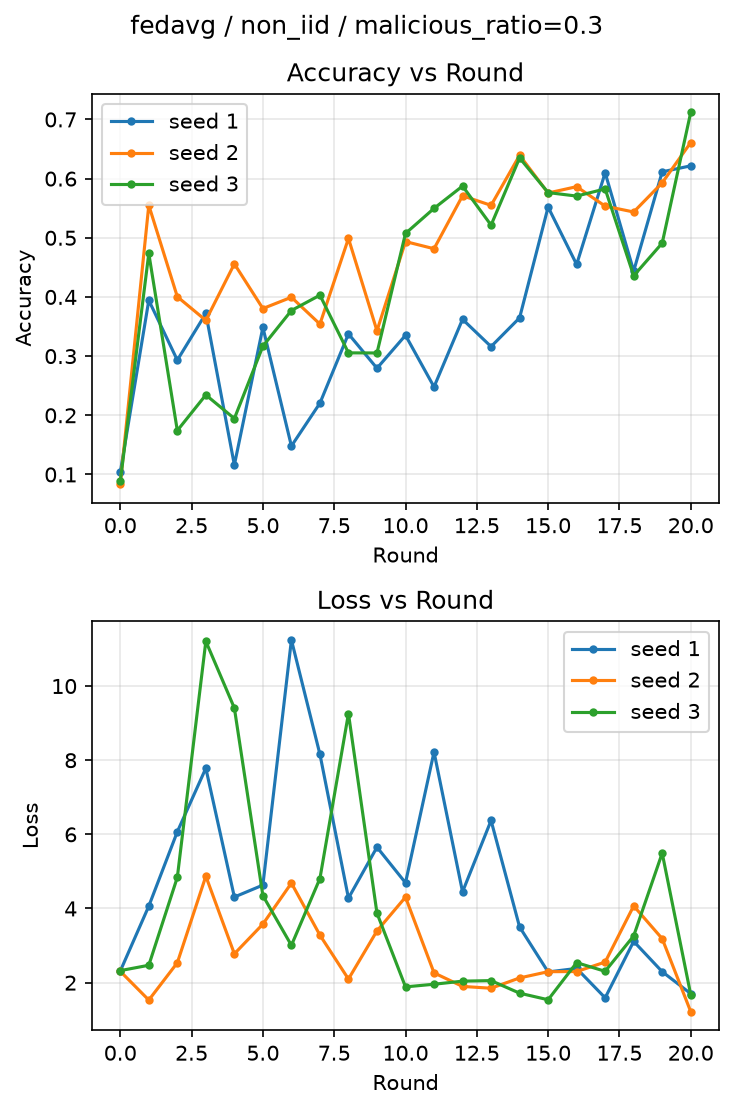
\includegraphics[width=\columnwidth]{seed_curves_noniid_ratio0.3.png}
    \caption{Seed ごとの Round-Accuracy および Round-Loss の推移（Non-IID，悪性クライアント比率 0.3）}
    \label{fig:seed_curves_noniid_ratio0.3}
\end{figure}
% =========================================================
\subsubsection{結果}
% =========================================================

表\ref{tab:fedavg_noniid_ratio0.3}に，各ラウンドにおける
Accuracy および Loss を示す．

学習開始時（Round 0）の Accuracy は約 0.08--0.10 であったが，
Round 1 では約 0.39--0.56 まで上昇した．
しかし悪性クライアント比率 0.2 の場合よりもさらに不安定な挙動を示し，
Round 6（Seed 1）で Loss が最大 11.2444 に達するなど，
学習全体を通じて Accuracy・Loss ともに大きな振動が続いた．
Round 20 時点の Accuracy は約 0.62--0.71，Loss は約 1.22--1.70 であった．

Non-IID 環境における悪性クライアント比率 0.0--0.2 の場合と比較すると，
悪性クライアント比率が高くなるほど Scale Attack を受けた更新が
単純平均に混入する割合が増え，IID 環境の同条件（1.4 節）と同様に
学習が大きく不安定化することが確認された．

\clearpage
% =========================================================
\subsection{FedAvg：Non-IID・悪性クライアント比率別の比較（Seed 1）}
% =========================================================

\subsubsection{実験条件}

\begin{itemize}
    \item \textbf{Aggregation method:} FedAvg
    \item \textbf{Data split:} Non-IID
    \item \textbf{Malicious ratio:} 0.0, 0.1, 0.2, 0.3
    \item \textbf{Attack:} Adaptive attack
    \item \textbf{Number of rounds:} 20
    \item \textbf{Seed:} 1
\end{itemize}

2.1--2.4 節で示した Seed 1 の結果を malicious ratio 別に
1つの図上で比較できるよう再構成した．
図の作成には \verb|result/plot_fedavg_iid_seed1_by_ratio.py| を
\verb|--split non_iid| オプションで用い，
\verb|result/results.csv| から FedAvg・Non-IID・seed=1 の条件に一致する
run を malicious ratio ごとに抽出して描画した．

% =========================================================
% 実験結果図
% =========================================================

\begin{figure}[H]
    \centering
    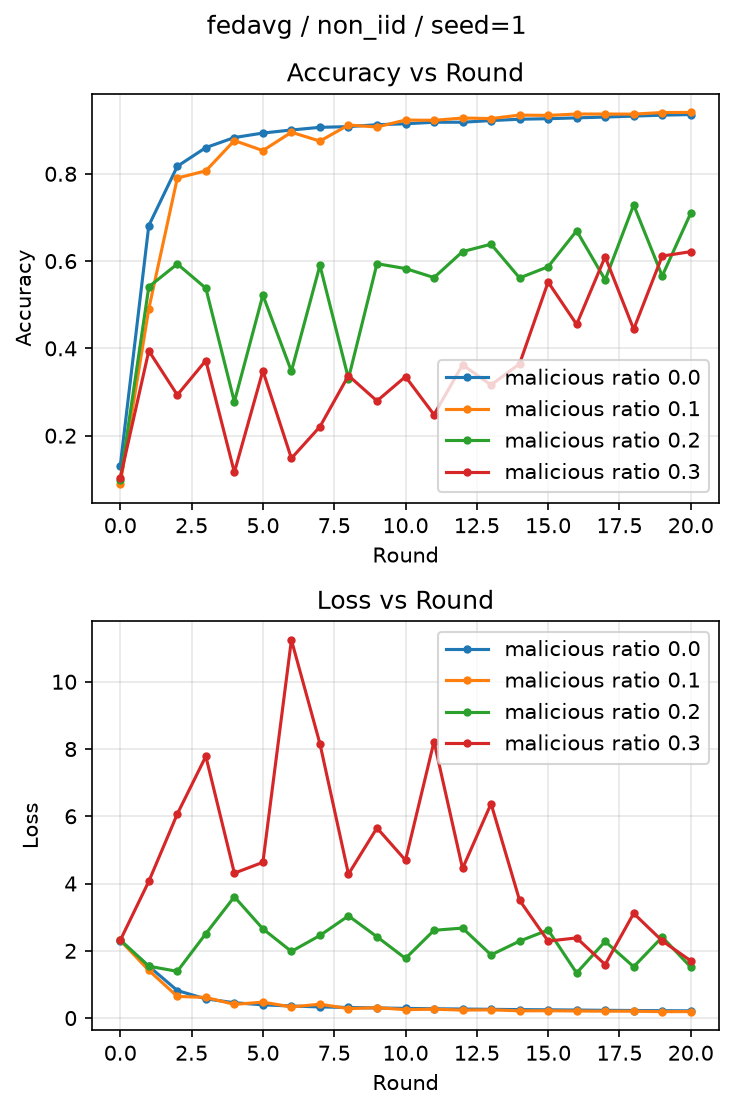
\includegraphics[width=\columnwidth]{fedavg_noniid_seed1_by_ratio.png}
    \caption{FedAvg・Non-IID・Seed 1 における malicious ratio 別の
    Round-Accuracy および Round-Loss の推移}
    \label{fig:fedavg_noniid_seed1_by_ratio}
\end{figure}

% =========================================================
\subsubsection{結果}
% =========================================================

図\ref{fig:fedavg_noniid_seed1_by_ratio}に，malicious ratio
0.0, 0.1, 0.2, 0.3 における Round-Accuracy および Round-Loss の推移を示す．

malicious ratio 0.0, 0.1 では Round 5 以降 Accuracy がおおむね
単調に向上し，Round 20 時点でそれぞれ 0.9358，0.9407 に達した．
一方 malicious ratio 0.2, 0.3 では Round 2 以降 Accuracy が
単調に向上せず，Round 20 まで大きく上下する不安定な挙動が続き，
Round 20 時点の Accuracy はそれぞれ 0.7097，0.6216 にとどまった．
Loss についても malicious ratio 0.2, 0.3 では学習全体を通じて
繰り返し急激なスパイクが見られ，malicious ratio 0.0, 0.1 のように
単調に減少する傾向は確認できなかった．

以上より，Non-IID 環境かつ Seed 1 において，
FedAvg は malicious ratio 0.1 までは希釈効果によって
安定した学習性能を維持できるものの，malicious ratio 0.2 以上では
Scale Attack を受けた悪性更新が単純平均に大きく混入し，
IID 環境（1.5 節）と同様に学習の不安定化・性能低下を招くことが
確認された．

\clearpage
% =========================================================
\section{Median（IID環境）における悪性クライアント比率別の評価}
% =========================================================

% =========================================================
\subsection{Median：IID・悪性クライアント比率 0.0}
% =========================================================

\subsubsection{実験条件}

\begin{itemize}
    \item \textbf{Aggregation method:} Median
    \item \textbf{Data split:} IID
    \item \textbf{Malicious ratio:} 0.0
    \item \textbf{Attack:} Adaptive attack
    \item \textbf{Number of rounds:} 20
    \item \textbf{Seeds:} 1, 2, 3
\end{itemize}

% =========================================================
% 実験結果表
% =========================================================

\begin{table}[H]
\centering

\caption{Median（IID，悪性クライアント比率 0.0）における
Accuracy および Loss}

\label{tab:median_iid_ratio0.0}

\footnotesize
\setlength{\tabcolsep}{2.5pt}
\renewcommand{\arraystretch}{0.90}

\resizebox{\columnwidth}{!}{%
\begin{tabular}{c cc cc cc}

\toprule

& \multicolumn{2}{c}{Seed 1}
& \multicolumn{2}{c}{Seed 2}
& \multicolumn{2}{c}{Seed 3} \\

\cmidrule(lr){2-3}
\cmidrule(lr){4-5}
\cmidrule(lr){6-7}

Round
& Acc. & Loss
& Acc. & Loss
& Acc. & Loss \\

\midrule

0 & 0.0920 & 2.3222 & 0.1002 & 2.3056 & 0.1309 & 2.3169 \\
1 & 0.6707 & 1.3895 & 0.7539 & 1.2184 & 0.7083 & 1.3385 \\
2 & 0.8524 & 0.6531 & 0.8498 & 0.6177 & 0.8397 & 0.6401 \\
3 & 0.8798 & 0.4794 & 0.8811 & 0.4668 & 0.8745 & 0.4841 \\
4 & 0.8915 & 0.4026 & 0.8931 & 0.3965 & 0.8922 & 0.4079 \\
5 & 0.8998 & 0.3609 & 0.9004 & 0.3554 & 0.9010 & 0.3630 \\
6 & 0.9073 & 0.3321 & 0.9060 & 0.3290 & 0.9064 & 0.3351 \\
7 & 0.9116 & 0.3121 & 0.9101 & 0.3087 & 0.9103 & 0.3150 \\
8 & 0.9148 & 0.2963 & 0.9150 & 0.2942 & 0.9128 & 0.2993 \\
9 & 0.9175 & 0.2848 & 0.9175 & 0.2810 & 0.9157 & 0.2868 \\
10 & 0.9192 & 0.2748 & 0.9210 & 0.2700 & 0.9178 & 0.2778 \\
11 & 0.9210 & 0.2650 & 0.9229 & 0.2590 & 0.9201 & 0.2672 \\
12 & 0.9245 & 0.2559 & 0.9244 & 0.2504 & 0.9217 & 0.2596 \\
13 & 0.9257 & 0.2482 & 0.9272 & 0.2416 & 0.9237 & 0.2515 \\
14 & 0.9268 & 0.2421 & 0.9303 & 0.2333 & 0.9263 & 0.2452 \\
15 & 0.9291 & 0.2354 & 0.9316 & 0.2280 & 0.9278 & 0.2389 \\
16 & 0.9316 & 0.2284 & 0.9330 & 0.2192 & 0.9297 & 0.2303 \\
17 & 0.9324 & 0.2232 & 0.9351 & 0.2137 & 0.9312 & 0.2244 \\
18 & 0.9341 & 0.2179 & 0.9385 & 0.2070 & 0.9348 & 0.2186 \\
19 & 0.9369 & 0.2115 & 0.9390 & 0.2023 & 0.9351 & 0.2131 \\
20 & 0.9382 & 0.2073 & 0.9412 & 0.1964 & 0.9363 & 0.2081 \\

\bottomrule

\end{tabular}%
}

\end{table}
\begin{figure}[H]
    \centering
    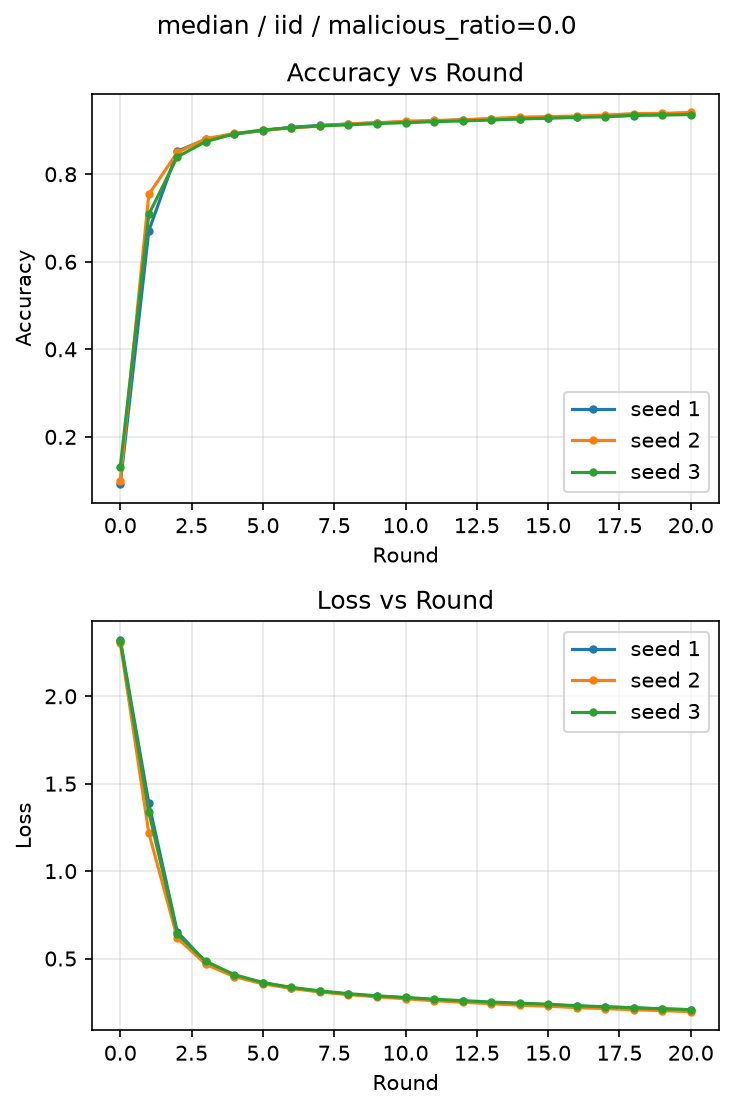
\includegraphics[width=\columnwidth]{seed_curves_median_iid_ratio0.0.png}
    \caption{Seed ごとの Round-Accuracy および Round-Loss の推移（IID，悪性クライアント比率 0.0）}
    \label{fig:seed_curves_median_iid_ratio0.0}
\end{figure}
% =========================================================
\subsubsection{結果}
% =========================================================

表\ref{tab:median_iid_ratio0.0}に，各ラウンドにおける
Accuracy および Loss を示す．

学習開始時（Round 0）の Accuracy は約 0.0920--0.1309 であったが，Round 1 では約 0.6707--0.7539 まで上昇した． その後も学習ラウンドの進行に伴って Accuracy は継続的に向上し，Round 20 ではすべての Seed において約 0.9363--0.9412 に達した． Round 20 時点の Loss は約 0.1964--0.2081 であった．

\clearpage
% =========================================================
\subsection{Median：IID・悪性クライアント比率 0.1}
% =========================================================

\subsubsection{実験条件}

\begin{itemize}
    \item \textbf{Aggregation method:} Median
    \item \textbf{Data split:} IID
    \item \textbf{Malicious ratio:} 0.1
    \item \textbf{Attack:} Adaptive attack
    \item \textbf{Number of rounds:} 20
    \item \textbf{Seeds:} 1, 2, 3
\end{itemize}

% =========================================================
% 実験結果表
% =========================================================

\begin{table}[H]
\centering

\caption{Median（IID，悪性クライアント比率 0.1）における
Accuracy および Loss}

\label{tab:median_iid_ratio0.1}

\footnotesize
\setlength{\tabcolsep}{2.5pt}
\renewcommand{\arraystretch}{0.90}

\resizebox{\columnwidth}{!}{%
\begin{tabular}{c cc cc cc}

\toprule

& \multicolumn{2}{c}{Seed 1}
& \multicolumn{2}{c}{Seed 2}
& \multicolumn{2}{c}{Seed 3} \\

\cmidrule(lr){2-3}
\cmidrule(lr){4-5}
\cmidrule(lr){6-7}

Round
& Acc. & Loss
& Acc. & Loss
& Acc. & Loss \\

\midrule

0 & 0.0864 & 2.3117 & 0.0914 & 2.3142 & 0.0470 & 2.3312 \\
1 & 0.7043 & 1.4725 & 0.7119 & 1.3667 & 0.7142 & 1.3878 \\
2 & 0.8397 & 0.7079 & 0.8440 & 0.6816 & 0.8331 & 0.7078 \\
3 & 0.8711 & 0.5224 & 0.8716 & 0.5084 & 0.8689 & 0.5274 \\
4 & 0.8870 & 0.4385 & 0.8878 & 0.4291 & 0.8837 & 0.4419 \\
5 & 0.8942 & 0.3918 & 0.8956 & 0.3848 & 0.8911 & 0.3954 \\
6 & 0.8990 & 0.3639 & 0.9009 & 0.3565 & 0.8973 & 0.3651 \\
7 & 0.9038 & 0.3436 & 0.9054 & 0.3360 & 0.9023 & 0.3432 \\
8 & 0.9070 & 0.3284 & 0.9079 & 0.3212 & 0.9057 & 0.3268 \\
9 & 0.9091 & 0.3164 & 0.9127 & 0.3083 & 0.9075 & 0.3142 \\
10 & 0.9117 & 0.3069 & 0.9145 & 0.2976 & 0.9098 & 0.3043 \\
11 & 0.9126 & 0.2982 & 0.9171 & 0.2895 & 0.9123 & 0.2953 \\
12 & 0.9147 & 0.2908 & 0.9192 & 0.2815 & 0.9141 & 0.2870 \\
13 & 0.9158 & 0.2854 & 0.9199 & 0.2750 & 0.9163 & 0.2801 \\
14 & 0.9179 & 0.2798 & 0.9211 & 0.2682 & 0.9173 & 0.2738 \\
15 & 0.9193 & 0.2731 & 0.9236 & 0.2624 & 0.9188 & 0.2682 \\
16 & 0.9206 & 0.2679 & 0.9257 & 0.2569 & 0.9203 & 0.2631 \\
17 & 0.9217 & 0.2638 & 0.9269 & 0.2520 & 0.9216 & 0.2586 \\
18 & 0.9223 & 0.2600 & 0.9281 & 0.2474 & 0.9231 & 0.2534 \\
19 & 0.9228 & 0.2551 & 0.9282 & 0.2436 & 0.9245 & 0.2490 \\
20 & 0.9243 & 0.2511 & 0.9297 & 0.2389 & 0.9258 & 0.2452 \\

\bottomrule

\end{tabular}%
}

\end{table}
\begin{figure}[H]
    \centering
    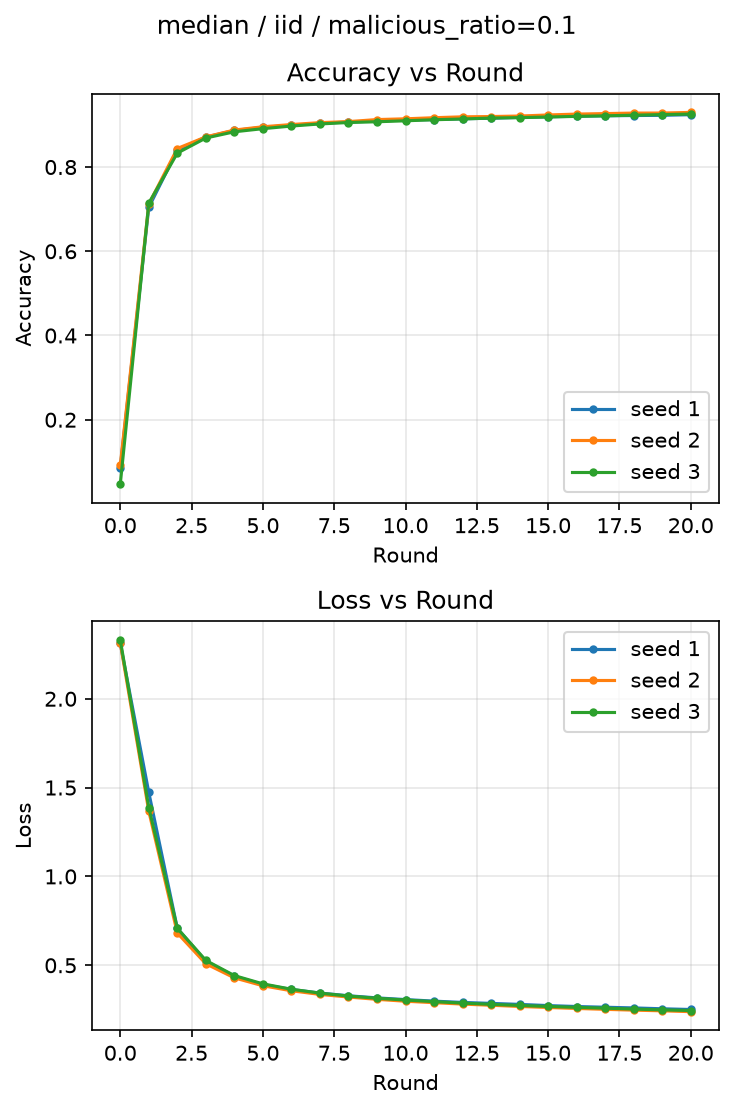
\includegraphics[width=\columnwidth]{seed_curves_median_iid_ratio0.1.png}
    \caption{Seed ごとの Round-Accuracy および Round-Loss の推移（IID，悪性クライアント比率 0.1）}
    \label{fig:seed_curves_median_iid_ratio0.1}
\end{figure}
% =========================================================
\subsubsection{結果}
% =========================================================

表\ref{tab:median_iid_ratio0.1}に，各ラウンドにおける
Accuracy および Loss を示す．

学習開始時（Round 0）の Accuracy は約 0.0470--0.0914 であったが，Round 1 では約 0.7043--0.7142 まで上昇した． その後も学習ラウンドの進行に伴って Accuracy は継続的に向上し，Round 20 ではすべての Seed において約 0.9243--0.9297 に達した． Round 20 時点の Loss は約 0.2389--0.2511 であった． 悪性クライアント比率 0.0 の場合（最終 Accuracy 平均 約 0.9386）と比較しても最終的な Accuracy に大きな差は見られず，本条件下でも学習は概ね安定していたといえる．

\clearpage
% =========================================================
\subsection{Median：IID・悪性クライアント比率 0.2}
% =========================================================

\subsubsection{実験条件}

\begin{itemize}
    \item \textbf{Aggregation method:} Median
    \item \textbf{Data split:} IID
    \item \textbf{Malicious ratio:} 0.2
    \item \textbf{Attack:} Adaptive attack
    \item \textbf{Number of rounds:} 20
    \item \textbf{Seeds:} 1, 2, 3
\end{itemize}

% =========================================================
% 実験結果表
% =========================================================

\begin{table}[H]
\centering

\caption{Median（IID，悪性クライアント比率 0.2）における
Accuracy および Loss}

\label{tab:median_iid_ratio0.2}

\footnotesize
\setlength{\tabcolsep}{2.5pt}
\renewcommand{\arraystretch}{0.90}

\resizebox{\columnwidth}{!}{%
\begin{tabular}{c cc cc cc}

\toprule

& \multicolumn{2}{c}{Seed 1}
& \multicolumn{2}{c}{Seed 2}
& \multicolumn{2}{c}{Seed 3} \\

\cmidrule(lr){2-3}
\cmidrule(lr){4-5}
\cmidrule(lr){6-7}

Round
& Acc. & Loss
& Acc. & Loss
& Acc. & Loss \\

\midrule

0 & 0.1052 & 2.3015 & 0.0847 & 2.3004 & 0.0985 & 2.3052 \\
1 & 0.7361 & 1.4644 & 0.7553 & 1.4592 & 0.6629 & 1.5615 \\
2 & 0.8356 & 0.7316 & 0.8405 & 0.7304 & 0.8304 & 0.7535 \\
3 & 0.8623 & 0.5486 & 0.8694 & 0.5446 & 0.8692 & 0.5463 \\
4 & 0.8773 & 0.4716 & 0.8818 & 0.4623 & 0.8816 & 0.4594 \\
5 & 0.8884 & 0.4279 & 0.8895 & 0.4171 & 0.8914 & 0.4111 \\
6 & 0.8919 & 0.4005 & 0.8947 & 0.3886 & 0.8956 & 0.3829 \\
7 & 0.8944 & 0.3810 & 0.8976 & 0.3698 & 0.8988 & 0.3627 \\
8 & 0.8971 & 0.3675 & 0.8998 & 0.3557 & 0.9019 & 0.3475 \\
9 & 0.8984 & 0.3561 & 0.9028 & 0.3460 & 0.9041 & 0.3360 \\
10 & 0.9005 & 0.3473 & 0.9039 & 0.3377 & 0.9060 & 0.3268 \\
11 & 0.9021 & 0.3394 & 0.9046 & 0.3307 & 0.9073 & 0.3197 \\
12 & 0.9036 & 0.3335 & 0.9061 & 0.3252 & 0.9085 & 0.3135 \\
13 & 0.9048 & 0.3283 & 0.9072 & 0.3202 & 0.9101 & 0.3075 \\
14 & 0.9051 & 0.3236 & 0.9083 & 0.3160 & 0.9102 & 0.3031 \\
15 & 0.9067 & 0.3202 & 0.9098 & 0.3122 & 0.9112 & 0.2997 \\
16 & 0.9077 & 0.3166 & 0.9100 & 0.3091 & 0.9122 & 0.2965 \\
17 & 0.9082 & 0.3132 & 0.9103 & 0.3063 & 0.9131 & 0.2928 \\
18 & 0.9087 & 0.3108 & 0.9115 & 0.3033 & 0.9128 & 0.2902 \\
19 & 0.9100 & 0.3080 & 0.9121 & 0.3010 & 0.9140 & 0.2876 \\
20 & 0.9102 & 0.3056 & 0.9124 & 0.2992 & 0.9147 & 0.2849 \\

\bottomrule

\end{tabular}%
}

\end{table}
\begin{figure}[H]
    \centering
    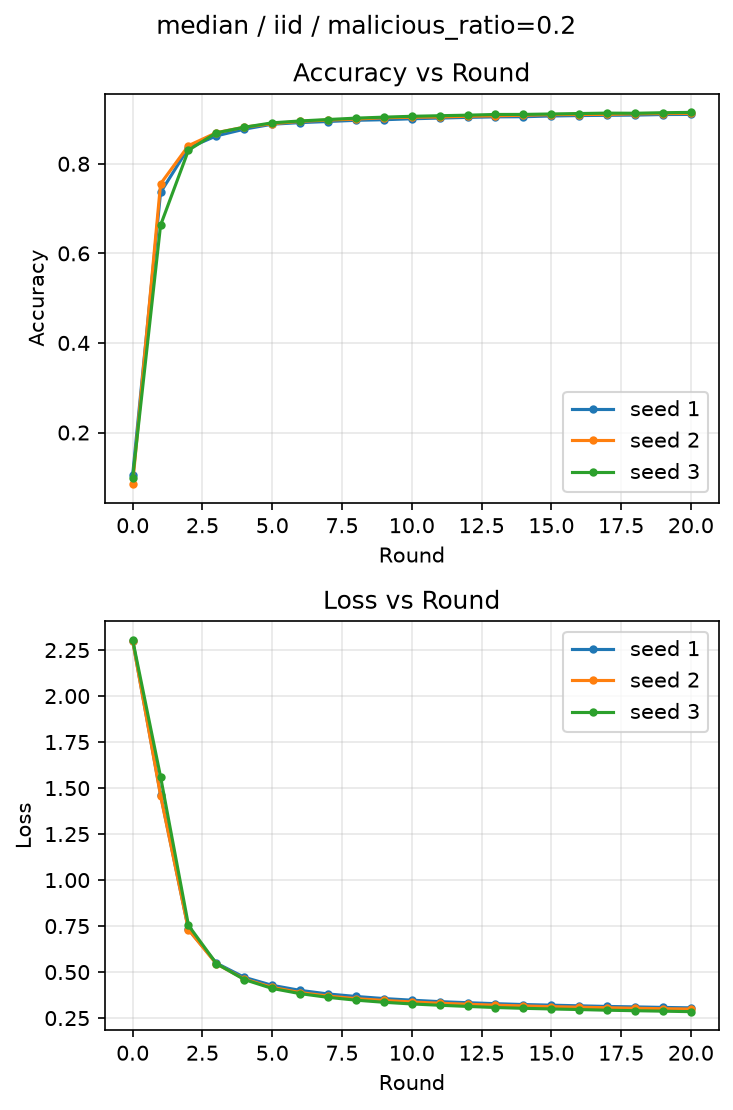
\includegraphics[width=\columnwidth]{seed_curves_median_iid_ratio0.2.png}
    \caption{Seed ごとの Round-Accuracy および Round-Loss の推移（IID，悪性クライアント比率 0.2）}
    \label{fig:seed_curves_median_iid_ratio0.2}
\end{figure}
% =========================================================
\subsubsection{結果}
% =========================================================

表\ref{tab:median_iid_ratio0.2}に，各ラウンドにおける
Accuracy および Loss を示す．

学習開始時（Round 0）の Accuracy は約 0.0847--0.1052 であったが，Round 1 では約 0.6629--0.7553 まで上昇した． その後も学習ラウンドの進行に伴って Accuracy は継続的に向上し，Round 20 ではすべての Seed において約 0.9102--0.9147 に達した． Round 20 時点の Loss は約 0.2849--0.3056 であった． 悪性クライアント比率 0.0 の場合（最終 Accuracy 平均 約 0.9386）と比較すると，本条件では約 0.0261 ポイント低い水準にとどまっており，悪性クライアント比率 0.2 における攻撃の影響が最終的な Accuracy にも現れていることが分かる．

\clearpage
% =========================================================
\subsection{Median：IID・悪性クライアント比率 0.3}
% =========================================================

\subsubsection{実験条件}

\begin{itemize}
    \item \textbf{Aggregation method:} Median
    \item \textbf{Data split:} IID
    \item \textbf{Malicious ratio:} 0.3
    \item \textbf{Attack:} Adaptive attack
    \item \textbf{Number of rounds:} 20
    \item \textbf{Seeds:} 1, 2, 3
\end{itemize}

% =========================================================
% 実験結果表
% =========================================================

\begin{table}[H]
\centering

\caption{Median（IID，悪性クライアント比率 0.3）における
Accuracy および Loss}

\label{tab:median_iid_ratio0.3}

\footnotesize
\setlength{\tabcolsep}{2.5pt}
\renewcommand{\arraystretch}{0.90}

\resizebox{\columnwidth}{!}{%
\begin{tabular}{c cc cc cc}

\toprule

& \multicolumn{2}{c}{Seed 1}
& \multicolumn{2}{c}{Seed 2}
& \multicolumn{2}{c}{Seed 3} \\

\cmidrule(lr){2-3}
\cmidrule(lr){4-5}
\cmidrule(lr){6-7}

Round
& Acc. & Loss
& Acc. & Loss
& Acc. & Loss \\

\midrule

0 & 0.0800 & 2.3165 & 0.1000 & 2.3002 & 0.0886 & 2.3121 \\
1 & 0.6250 & 1.7308 & 0.6776 & 1.6286 & 0.7264 & 1.5433 \\
2 & 0.8050 & 0.9383 & 0.8072 & 0.8780 & 0.8521 & 0.7929 \\
3 & 0.8509 & 0.6628 & 0.8510 & 0.6317 & 0.8715 & 0.5849 \\
4 & 0.8694 & 0.5526 & 0.8703 & 0.5343 & 0.8803 & 0.5067 \\
5 & 0.8766 & 0.4956 & 0.8810 & 0.4804 & 0.8844 & 0.4648 \\
6 & 0.8835 & 0.4619 & 0.8847 & 0.4514 & 0.8882 & 0.4399 \\
7 & 0.8872 & 0.4405 & 0.8864 & 0.4300 & 0.8893 & 0.4234 \\
8 & 0.8893 & 0.4251 & 0.8887 & 0.4155 & 0.8888 & 0.4136 \\
9 & 0.8900 & 0.4146 & 0.8890 & 0.4066 & 0.8895 & 0.4069 \\
10 & 0.8899 & 0.4084 & 0.8911 & 0.3993 & 0.8897 & 0.4006 \\
11 & 0.8912 & 0.4035 & 0.8918 & 0.3940 & 0.8897 & 0.3958 \\
12 & 0.8907 & 0.3984 & 0.8919 & 0.3897 & 0.8908 & 0.3929 \\
13 & 0.8910 & 0.3943 & 0.8923 & 0.3864 & 0.8915 & 0.3903 \\
14 & 0.8930 & 0.3916 & 0.8926 & 0.3825 & 0.8931 & 0.3861 \\
15 & 0.8938 & 0.3872 & 0.8941 & 0.3792 & 0.8929 & 0.3839 \\
16 & 0.8927 & 0.3851 & 0.8936 & 0.3773 & 0.8928 & 0.3832 \\
17 & 0.8936 & 0.3831 & 0.8926 & 0.3764 & 0.8933 & 0.3793 \\
18 & 0.8937 & 0.3828 & 0.8946 & 0.3719 & 0.8934 & 0.3779 \\
19 & 0.8944 & 0.3795 & 0.8941 & 0.3720 & 0.8941 & 0.3772 \\
20 & 0.8945 & 0.3777 & 0.8952 & 0.3666 & 0.8948 & 0.3742 \\

\bottomrule

\end{tabular}%
}

\end{table}
\begin{figure}[H]
    \centering
    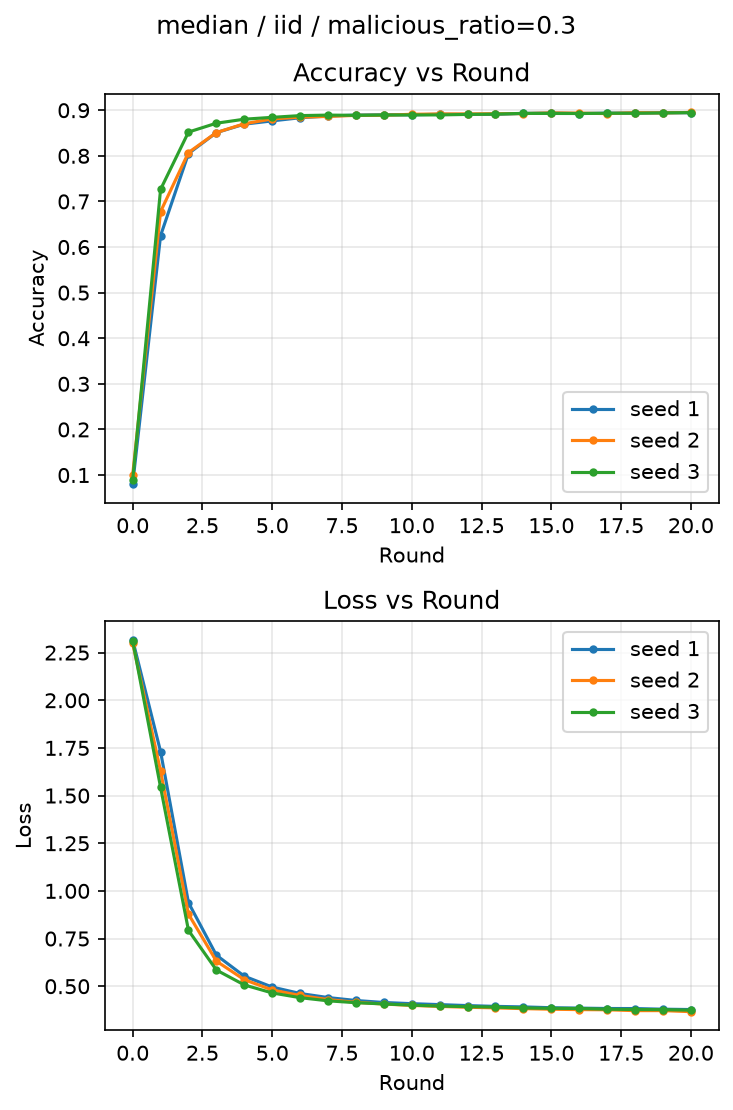
\includegraphics[width=\columnwidth]{seed_curves_median_iid_ratio0.3.png}
    \caption{Seed ごとの Round-Accuracy および Round-Loss の推移（IID，悪性クライアント比率 0.3）}
    \label{fig:seed_curves_median_iid_ratio0.3}
\end{figure}
% =========================================================
\subsubsection{結果}
% =========================================================

表\ref{tab:median_iid_ratio0.3}に，各ラウンドにおける
Accuracy および Loss を示す．

学習開始時（Round 0）の Accuracy は約 0.0800--0.1000 であったが，Round 1 では約 0.6250--0.7264 まで上昇した． その後も学習ラウンドの進行に伴って Accuracy は継続的に向上し，Round 20 ではすべての Seed において約 0.8945--0.8952 に達した． Round 20 時点の Loss は約 0.3666--0.3777 であった． 悪性クライアント比率 0.0 の場合（最終 Accuracy 平均 約 0.9386）と比較すると，本条件では約 0.0437 ポイント低い水準にとどまっており，悪性クライアント比率 0.3 における攻撃の影響が最終的な Accuracy にも現れていることが分かる．

\clearpage
% =========================================================
\subsection{Median：IID・悪性クライアント比率別の比較（Seed 1）}
% =========================================================

\subsubsection{実験条件}

\begin{itemize}
    \item \textbf{Aggregation method:} Median
    \item \textbf{Data split:} IID
    \item \textbf{Malicious ratio:} 0.0, 0.1, 0.2, 0.3
    \item \textbf{Attack:} Adaptive attack
    \item \textbf{Number of rounds:} 20
    \item \textbf{Seed:} 1
\end{itemize}

3.1--3.4 節で示した Seed 1 の結果を malicious ratio 別に
1つの図上で比較できるよう再構成した．
図の作成には \verb|result/plot_fedavg_iid_seed1_by_ratio.py| を
\verb|--aggregation median| オプションで用い，
\verb|result/results.csv| から Median・IID・seed=1 の条件に一致する
run を malicious ratio ごとに抽出して描画した．

% =========================================================
% 実験結果図
% =========================================================

\begin{figure}[H]
    \centering
    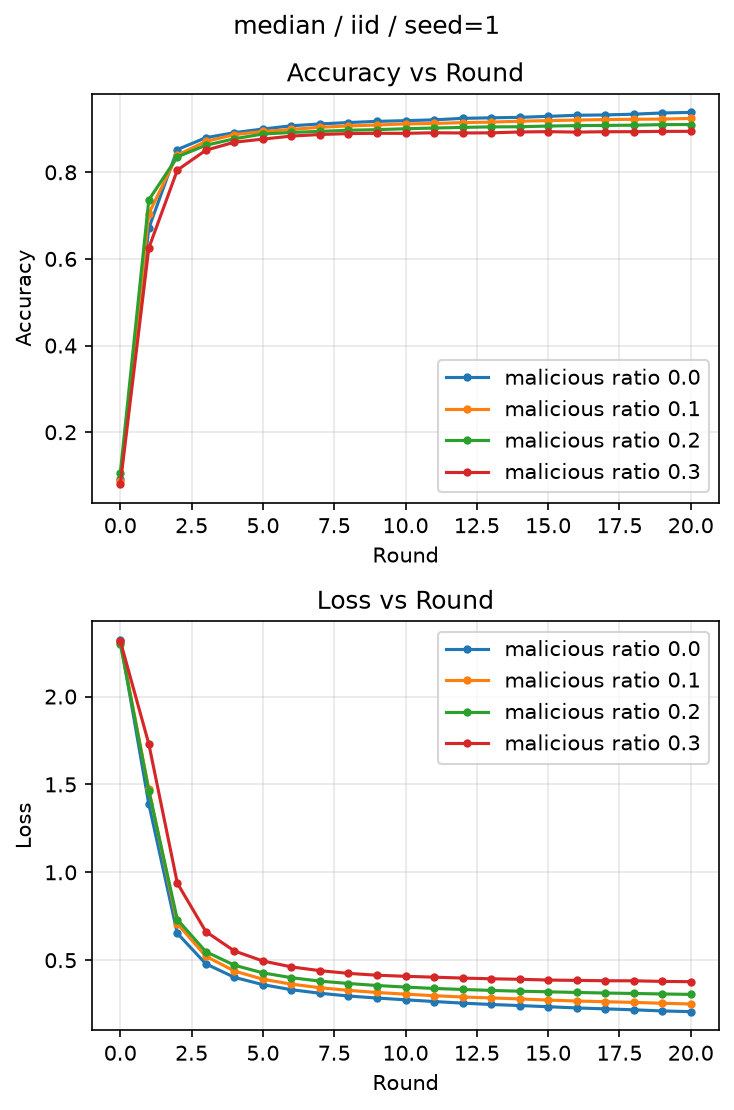
\includegraphics[width=\columnwidth]{median_iid_seed1_by_ratio.png}
    \caption{Median・IID・Seed 1 における malicious ratio 別の
    Round-Accuracy および Round-Loss の推移}
    \label{fig:median_iid_seed1_by_ratio}
\end{figure}

% =========================================================
\subsubsection{結果}
% =========================================================

図\ref{fig:median_iid_seed1_by_ratio}に，malicious ratio
0.0, 0.1, 0.2, 0.3 における Round-Accuracy および Round-Loss の推移を示す．

FedAvg の場合とは異なり，Median では malicious ratio の増加に伴って
Round 20 時点の Accuracy が 0.9382（ratio 0.0）から
0.9243（ratio 0.1），0.9102（ratio 0.2），0.8945（ratio 0.3）と
単調に低下する傾向が確認された．
Loss についても同様に，Round 20 時点で 0.2073（ratio 0.0）から
0.3777（ratio 0.3）まで malicious ratio の増加とともに増加しており，
学習の収束レベル自体が悪化していることが分かる．

以上より，IID 環境かつ Seed 1 において，
Median は malicious ratio の増加に対して FedAvg よりも
感度が高く，攻撃の影響がモデル性能に明確に現れることが確認された．

\clearpage
% =========================================================
\section{Median（Non-IID環境）における悪性クライアント比率別の評価}
% =========================================================

% =========================================================
\subsection{Median：Non-IID・悪性クライアント比率 0.0}
% =========================================================

\subsubsection{実験条件}

\begin{itemize}
    \item \textbf{Aggregation method:} Median
    \item \textbf{Data split:} Non-IID
    \item \textbf{Malicious ratio:} 0.0
    \item \textbf{Attack:} Adaptive attack
    \item \textbf{Number of rounds:} 20
    \item \textbf{Seeds:} 1, 2, 3
\end{itemize}

% =========================================================
% 実験結果表
% =========================================================

\begin{table}[H]
\centering

\caption{Median（Non-IID，悪性クライアント比率 0.0）における
Accuracy および Loss}

\label{tab:median_non_iid_ratio0.0}

\footnotesize
\setlength{\tabcolsep}{2.5pt}
\renewcommand{\arraystretch}{0.90}

\resizebox{\columnwidth}{!}{%
\begin{tabular}{c cc cc cc}

\toprule

& \multicolumn{2}{c}{Seed 1}
& \multicolumn{2}{c}{Seed 2}
& \multicolumn{2}{c}{Seed 3} \\

\cmidrule(lr){2-3}
\cmidrule(lr){4-5}
\cmidrule(lr){6-7}

Round
& Acc. & Loss
& Acc. & Loss
& Acc. & Loss \\

\midrule

0 & 0.0739 & 2.3070 & 0.1295 & 2.3105 & 0.1624 & 2.2938 \\
1 & 0.5701 & 1.6919 & 0.7103 & 1.6034 & 0.5807 & 1.6502 \\
2 & 0.7883 & 0.9640 & 0.7983 & 0.8726 & 0.7979 & 0.8801 \\
3 & 0.8517 & 0.6412 & 0.8486 & 0.6181 & 0.8569 & 0.6048 \\
4 & 0.8714 & 0.5074 & 0.8662 & 0.5056 & 0.8727 & 0.4905 \\
5 & 0.8822 & 0.4382 & 0.8848 & 0.4386 & 0.8899 & 0.4208 \\
6 & 0.8911 & 0.3945 & 0.8921 & 0.3975 & 0.8930 & 0.3846 \\
7 & 0.8974 & 0.3628 & 0.8997 & 0.3671 & 0.9019 & 0.3535 \\
8 & 0.9031 & 0.3424 & 0.9050 & 0.3429 & 0.9059 & 0.3340 \\
9 & 0.9068 & 0.3254 & 0.9094 & 0.3254 & 0.9084 & 0.3185 \\
10 & 0.9106 & 0.3107 & 0.9114 & 0.3117 & 0.9121 & 0.3060 \\
11 & 0.9131 & 0.2999 & 0.9139 & 0.2976 & 0.9144 & 0.2945 \\
12 & 0.9144 & 0.2901 & 0.9176 & 0.2889 & 0.9158 & 0.2877 \\
13 & 0.9170 & 0.2807 & 0.9194 & 0.2791 & 0.9195 & 0.2782 \\
14 & 0.9195 & 0.2729 & 0.9202 & 0.2704 & 0.9205 & 0.2707 \\
15 & 0.9221 & 0.2653 & 0.9223 & 0.2642 & 0.9222 & 0.2649 \\
16 & 0.9229 & 0.2587 & 0.9249 & 0.2571 & 0.9237 & 0.2573 \\
17 & 0.9251 & 0.2527 & 0.9254 & 0.2515 & 0.9251 & 0.2514 \\
18 & 0.9264 & 0.2468 & 0.9274 & 0.2442 & 0.9266 & 0.2463 \\
19 & 0.9279 & 0.2422 & 0.9289 & 0.2384 & 0.9280 & 0.2399 \\
20 & 0.9277 & 0.2356 & 0.9304 & 0.2329 & 0.9282 & 0.2350 \\

\bottomrule

\end{tabular}%
}

\end{table}
\begin{figure}[H]
    \centering
    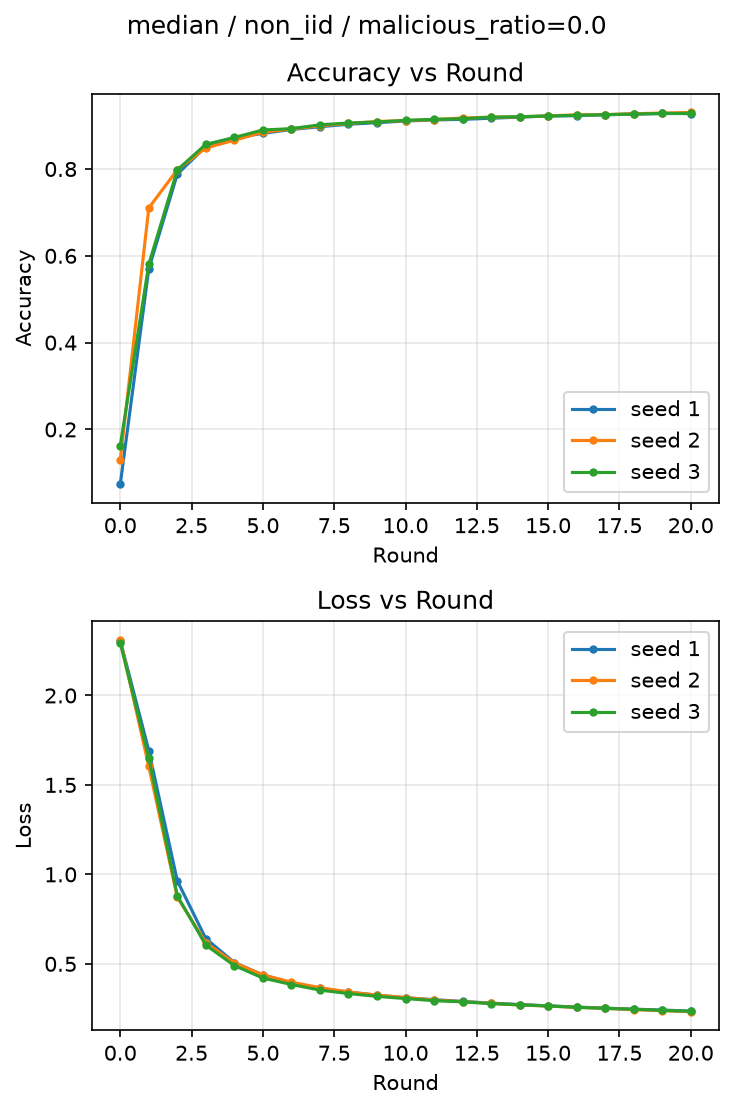
\includegraphics[width=\columnwidth]{seed_curves_median_non_iid_ratio0.0.png}
    \caption{Seed ごとの Round-Accuracy および Round-Loss の推移（Non-IID，悪性クライアント比率 0.0）}
    \label{fig:seed_curves_median_non_iid_ratio0.0}
\end{figure}
% =========================================================
\subsubsection{結果}
% =========================================================

表\ref{tab:median_non_iid_ratio0.0}に，各ラウンドにおける
Accuracy および Loss を示す．

学習開始時（Round 0）の Accuracy は約 0.0739--0.1624 であったが，Round 1 では約 0.5701--0.7103 まで上昇した． その後も学習ラウンドの進行に伴って Accuracy は継続的に向上し，Round 20 ではすべての Seed において約 0.9277--0.9304 に達した． Round 20 時点の Loss は約 0.2329--0.2356 であった．

\clearpage
% =========================================================
\subsection{Median：Non-IID・悪性クライアント比率 0.1}
% =========================================================

\subsubsection{実験条件}

\begin{itemize}
    \item \textbf{Aggregation method:} Median
    \item \textbf{Data split:} Non-IID
    \item \textbf{Malicious ratio:} 0.1
    \item \textbf{Attack:} Adaptive attack
    \item \textbf{Number of rounds:} 20
    \item \textbf{Seeds:} 1, 2, 3
\end{itemize}

% =========================================================
% 実験結果表
% =========================================================

\begin{table}[H]
\centering

\caption{Median（Non-IID，悪性クライアント比率 0.1）における
Accuracy および Loss}

\label{tab:median_non_iid_ratio0.1}

\footnotesize
\setlength{\tabcolsep}{2.5pt}
\renewcommand{\arraystretch}{0.90}

\resizebox{\columnwidth}{!}{%
\begin{tabular}{c cc cc cc}

\toprule

& \multicolumn{2}{c}{Seed 1}
& \multicolumn{2}{c}{Seed 2}
& \multicolumn{2}{c}{Seed 3} \\

\cmidrule(lr){2-3}
\cmidrule(lr){4-5}
\cmidrule(lr){6-7}

Round
& Acc. & Loss
& Acc. & Loss
& Acc. & Loss \\

\midrule

0 & 0.1143 & 2.3175 & 0.0843 & 2.3148 & 0.0806 & 2.3113 \\
1 & 0.6021 & 1.7772 & 0.5558 & 1.7669 & 0.6241 & 1.7200 \\
2 & 0.7833 & 1.0821 & 0.7791 & 1.0283 & 0.7799 & 1.0302 \\
3 & 0.8376 & 0.7353 & 0.8430 & 0.7026 & 0.8403 & 0.7245 \\
4 & 0.8629 & 0.5710 & 0.8623 & 0.5604 & 0.8635 & 0.5751 \\
5 & 0.8792 & 0.4806 & 0.8765 & 0.4823 & 0.8761 & 0.4935 \\
6 & 0.8865 & 0.4307 & 0.8851 & 0.4346 & 0.8868 & 0.4404 \\
7 & 0.8925 & 0.3969 & 0.8938 & 0.4010 & 0.8920 & 0.4049 \\
8 & 0.8990 & 0.3725 & 0.8969 & 0.3786 & 0.8962 & 0.3781 \\
9 & 0.9017 & 0.3549 & 0.9017 & 0.3614 & 0.9004 & 0.3588 \\
10 & 0.9037 & 0.3414 & 0.9034 & 0.3469 & 0.9026 & 0.3443 \\
11 & 0.9050 & 0.3302 & 0.9059 & 0.3350 & 0.9046 & 0.3324 \\
12 & 0.9080 & 0.3211 & 0.9069 & 0.3257 & 0.9072 & 0.3219 \\
13 & 0.9101 & 0.3133 & 0.9073 & 0.3182 & 0.9091 & 0.3130 \\
14 & 0.9104 & 0.3071 & 0.9101 & 0.3109 & 0.9111 & 0.3049 \\
15 & 0.9131 & 0.3008 & 0.9112 & 0.3053 & 0.9121 & 0.2989 \\
16 & 0.9120 & 0.2971 & 0.9129 & 0.2993 & 0.9149 & 0.2917 \\
17 & 0.9150 & 0.2911 & 0.9125 & 0.2947 & 0.9148 & 0.2875 \\
18 & 0.9163 & 0.2866 & 0.9138 & 0.2909 & 0.9164 & 0.2828 \\
19 & 0.9168 & 0.2827 & 0.9155 & 0.2856 & 0.9173 & 0.2778 \\
20 & 0.9167 & 0.2802 & 0.9161 & 0.2818 & 0.9179 & 0.2734 \\

\bottomrule

\end{tabular}%
}

\end{table}
\begin{figure}[H]
    \centering
    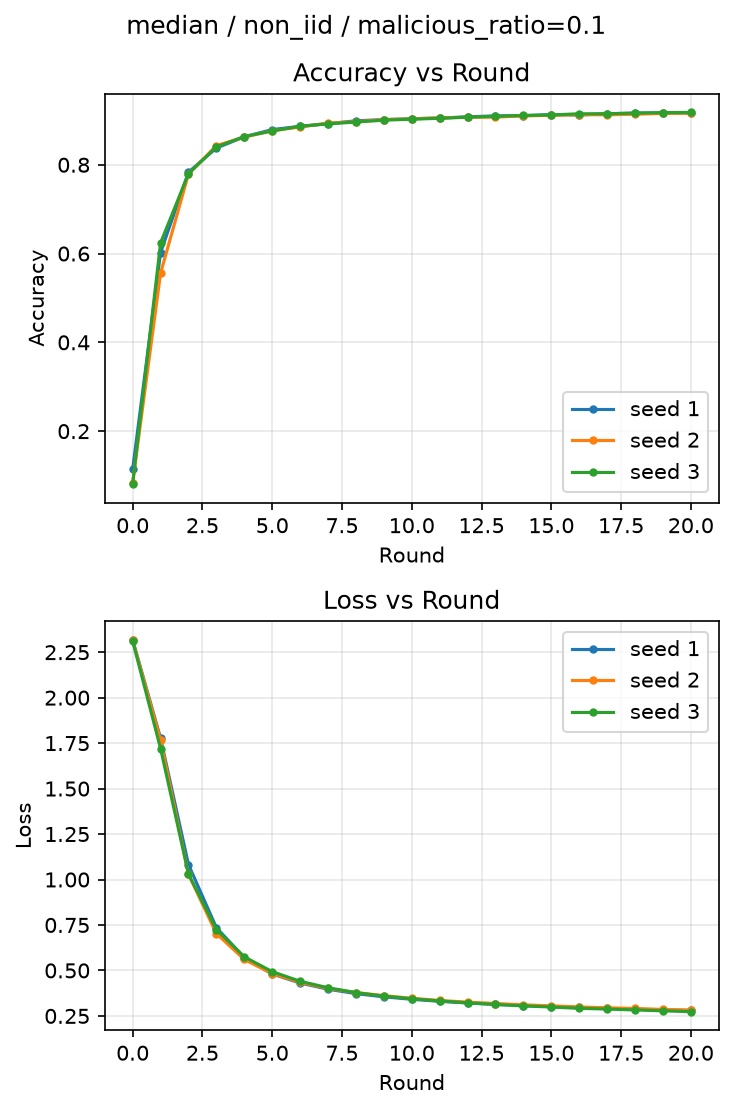
\includegraphics[width=\columnwidth]{seed_curves_median_non_iid_ratio0.1.png}
    \caption{Seed ごとの Round-Accuracy および Round-Loss の推移（Non-IID，悪性クライアント比率 0.1）}
    \label{fig:seed_curves_median_non_iid_ratio0.1}
\end{figure}
% =========================================================
\subsubsection{結果}
% =========================================================

表\ref{tab:median_non_iid_ratio0.1}に，各ラウンドにおける
Accuracy および Loss を示す．

学習開始時（Round 0）の Accuracy は約 0.0806--0.1143 であったが，Round 1 では約 0.5558--0.6241 まで上昇した． その後も学習ラウンドの進行に伴って Accuracy は継続的に向上し，Round 20 ではすべての Seed において約 0.9161--0.9179 に達した． Round 20 時点の Loss は約 0.2734--0.2818 であった． 悪性クライアント比率 0.0 の場合（最終 Accuracy 平均 約 0.9288）と比較しても最終的な Accuracy に大きな差は見られず，本条件下でも学習は概ね安定していたといえる．

\clearpage
% =========================================================
\subsection{Median：Non-IID・悪性クライアント比率 0.2}
% =========================================================

\subsubsection{実験条件}

\begin{itemize}
    \item \textbf{Aggregation method:} Median
    \item \textbf{Data split:} Non-IID
    \item \textbf{Malicious ratio:} 0.2
    \item \textbf{Attack:} Adaptive attack
    \item \textbf{Number of rounds:} 20
    \item \textbf{Seeds:} 1, 2, 3
\end{itemize}

% =========================================================
% 実験結果表
% =========================================================

\begin{table}[H]
\centering

\caption{Median（Non-IID，悪性クライアント比率 0.2）における
Accuracy および Loss}

\label{tab:median_non_iid_ratio0.2}

\footnotesize
\setlength{\tabcolsep}{2.5pt}
\renewcommand{\arraystretch}{0.90}

\resizebox{\columnwidth}{!}{%
\begin{tabular}{c cc cc cc}

\toprule

& \multicolumn{2}{c}{Seed 1}
& \multicolumn{2}{c}{Seed 2}
& \multicolumn{2}{c}{Seed 3} \\

\cmidrule(lr){2-3}
\cmidrule(lr){4-5}
\cmidrule(lr){6-7}

Round
& Acc. & Loss
& Acc. & Loss
& Acc. & Loss \\

\midrule

0 & 0.0911 & 2.2969 & 0.1224 & 2.3036 & 0.1257 & 2.3050 \\
1 & 0.5677 & 1.8220 & 0.5526 & 1.9451 & 0.5846 & 1.8880 \\
2 & 0.7379 & 1.1871 & 0.7254 & 1.3227 & 0.7990 & 1.2339 \\
3 & 0.7975 & 0.8622 & 0.7751 & 0.9226 & 0.8328 & 0.8586 \\
4 & 0.8345 & 0.6907 & 0.8212 & 0.7240 & 0.8513 & 0.6779 \\
5 & 0.8556 & 0.5938 & 0.8523 & 0.6147 & 0.8640 & 0.5822 \\
6 & 0.8659 & 0.5325 & 0.8652 & 0.5479 & 0.8714 & 0.5220 \\
7 & 0.8763 & 0.4894 & 0.8714 & 0.5044 & 0.8777 & 0.4808 \\
8 & 0.8815 & 0.4604 & 0.8785 & 0.4731 & 0.8853 & 0.4504 \\
9 & 0.8818 & 0.4402 & 0.8833 & 0.4497 & 0.8887 & 0.4305 \\
10 & 0.8860 & 0.4232 & 0.8874 & 0.4317 & 0.8909 & 0.4125 \\
11 & 0.8878 & 0.4094 & 0.8900 & 0.4165 & 0.8911 & 0.3999 \\
12 & 0.8914 & 0.3978 & 0.8904 & 0.4061 & 0.8947 & 0.3895 \\
13 & 0.8937 & 0.3873 & 0.8930 & 0.3939 & 0.8945 & 0.3817 \\
14 & 0.8956 & 0.3794 & 0.8962 & 0.3849 & 0.8968 & 0.3738 \\
15 & 0.8950 & 0.3743 & 0.8965 & 0.3781 & 0.8978 & 0.3668 \\
16 & 0.8954 & 0.3690 & 0.8970 & 0.3715 & 0.8993 & 0.3617 \\
17 & 0.8960 & 0.3644 & 0.8984 & 0.3666 & 0.8997 & 0.3560 \\
18 & 0.8961 & 0.3600 & 0.8995 & 0.3611 & 0.9008 & 0.3514 \\
19 & 0.8969 & 0.3573 & 0.9002 & 0.3565 & 0.8999 & 0.3482 \\
20 & 0.8979 & 0.3553 & 0.9013 & 0.3523 & 0.9014 & 0.3443 \\

\bottomrule

\end{tabular}%
}

\end{table}
\begin{figure}[H]
    \centering
    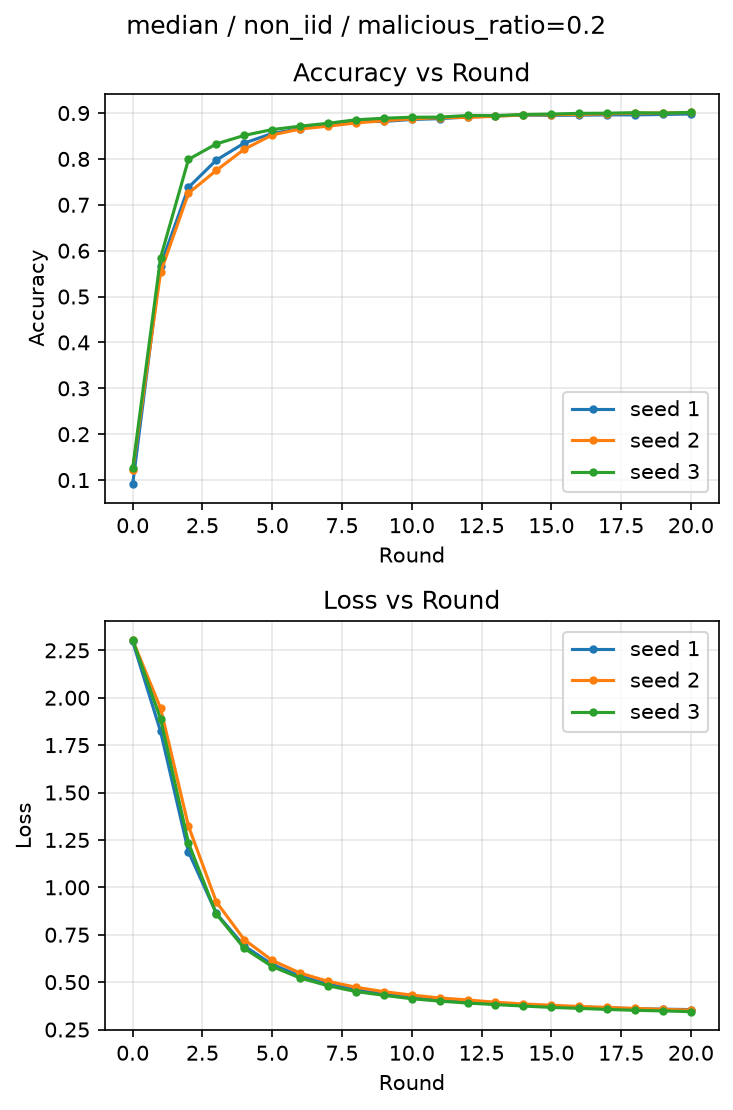
\includegraphics[width=\columnwidth]{seed_curves_median_non_iid_ratio0.2.png}
    \caption{Seed ごとの Round-Accuracy および Round-Loss の推移（Non-IID，悪性クライアント比率 0.2）}
    \label{fig:seed_curves_median_non_iid_ratio0.2}
\end{figure}
% =========================================================
\subsubsection{結果}
% =========================================================

表\ref{tab:median_non_iid_ratio0.2}に，各ラウンドにおける
Accuracy および Loss を示す．

学習開始時（Round 0）の Accuracy は約 0.0911--0.1257 であったが，Round 1 では約 0.5526--0.5846 まで上昇した． その後も学習ラウンドの進行に伴って Accuracy は継続的に向上し，Round 20 ではすべての Seed において約 0.8979--0.9014 に達した． Round 20 時点の Loss は約 0.3443--0.3553 であった． 悪性クライアント比率 0.0 の場合（最終 Accuracy 平均 約 0.9288）と比較すると，本条件では約 0.0286 ポイント低い水準にとどまっており，悪性クライアント比率 0.2 における攻撃の影響が最終的な Accuracy にも現れていることが分かる．

\clearpage
% =========================================================
\subsection{Median：Non-IID・悪性クライアント比率 0.3}
% =========================================================

\subsubsection{実験条件}

\begin{itemize}
    \item \textbf{Aggregation method:} Median
    \item \textbf{Data split:} Non-IID
    \item \textbf{Malicious ratio:} 0.3
    \item \textbf{Attack:} Adaptive attack
    \item \textbf{Number of rounds:} 20
    \item \textbf{Seeds:} 1, 2, 3
\end{itemize}

% =========================================================
% 実験結果表
% =========================================================

\begin{table}[H]
\centering

\caption{Median（Non-IID，悪性クライアント比率 0.3）における
Accuracy および Loss}

\label{tab:median_non_iid_ratio0.3}

\footnotesize
\setlength{\tabcolsep}{2.5pt}
\renewcommand{\arraystretch}{0.90}

\resizebox{\columnwidth}{!}{%
\begin{tabular}{c cc cc cc}

\toprule

& \multicolumn{2}{c}{Seed 1}
& \multicolumn{2}{c}{Seed 2}
& \multicolumn{2}{c}{Seed 3} \\

\cmidrule(lr){2-3}
\cmidrule(lr){4-5}
\cmidrule(lr){6-7}

Round
& Acc. & Loss
& Acc. & Loss
& Acc. & Loss \\

\midrule

0 & 0.1070 & 2.3018 & 0.1216 & 2.3113 & 0.0715 & 2.3203 \\
1 & 0.3900 & 2.1443 & 0.3576 & 2.1312 & 0.3943 & 2.1443 \\
2 & -- & -- & 0.5501 & 1.7567 & 0.5128 & 1.7931 \\
3 & -- & -- & 0.6893 & 1.4342 & 0.5995 & 1.4543 \\
4 & -- & -- & 0.7622 & 1.1808 & 0.6662 & 1.2061 \\
5 & -- & -- & 0.7979 & 0.9980 & 0.7248 & 1.0318 \\
6 & -- & -- & 0.8282 & 0.8638 & 0.7756 & 0.9011 \\
7 & -- & -- & 0.8364 & 0.7795 & 0.8144 & 0.8137 \\
8 & -- & -- & 0.8458 & 0.7181 & 0.8209 & 0.7454 \\
9 & -- & -- & 0.8569 & 0.6727 & 0.8295 & 0.6967 \\
10 & -- & -- & 0.8586 & 0.6420 & 0.8403 & 0.6638 \\
11 & -- & -- & 0.8647 & 0.6116 & 0.8454 & 0.6354 \\
12 & -- & -- & 0.8636 & 0.5942 & 0.8511 & 0.6135 \\
13 & -- & -- & 0.8671 & 0.5746 & 0.8523 & 0.5980 \\
14 & -- & -- & 0.8703 & 0.5580 & 0.8580 & 0.5827 \\
15 & -- & -- & 0.8719 & 0.5447 & 0.8586 & 0.5737 \\
16 & -- & -- & 0.8714 & 0.5376 & 0.8606 & 0.5587 \\
17 & -- & -- & 0.8729 & 0.5289 & 0.8621 & 0.5499 \\
18 & -- & -- & 0.8748 & 0.5208 & 0.8650 & 0.5419 \\
19 & -- & -- & 0.8760 & 0.5178 & 0.8658 & 0.5370 \\
20 & -- & -- & 0.8754 & 0.5147 & 0.8649 & 0.5291 \\

\bottomrule

\end{tabular}%
}

\end{table}
\begin{figure}[H]
    \centering
    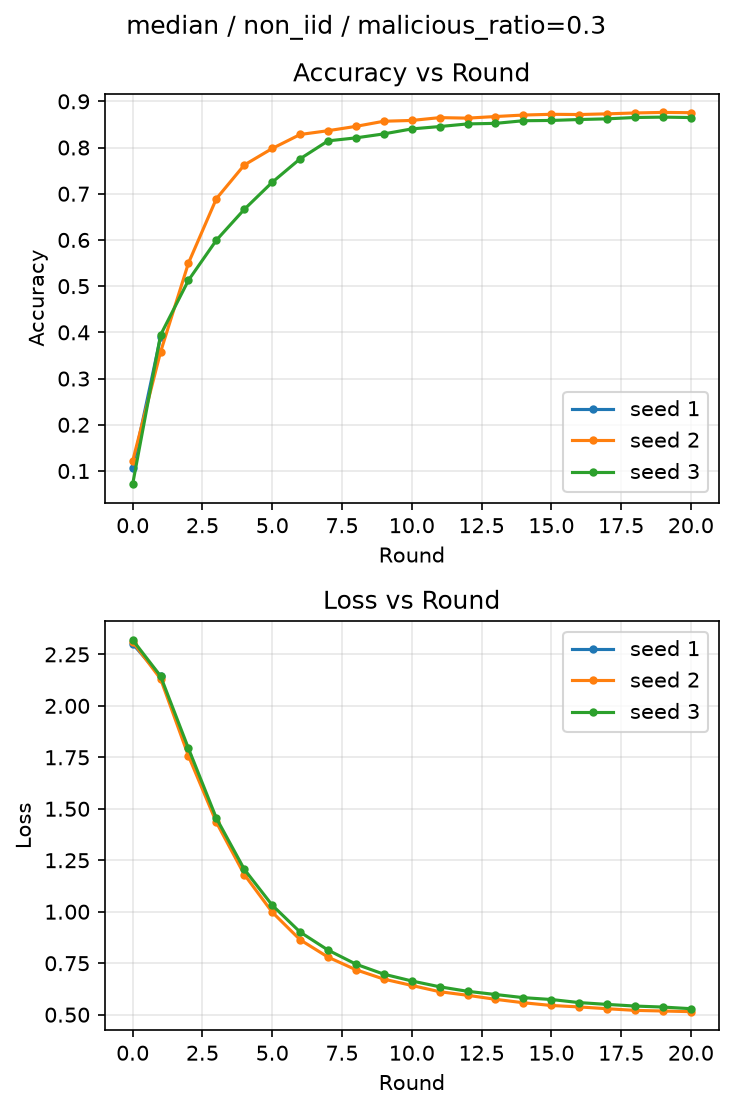
\includegraphics[width=\columnwidth]{seed_curves_median_non_iid_ratio0.3.png}
    \caption{Seed ごとの Round-Accuracy および Round-Loss の推移（Non-IID，悪性クライアント比率 0.3）}
    \label{fig:seed_curves_median_non_iid_ratio0.3}
\end{figure}
% =========================================================
\subsubsection{結果}
% =========================================================

表\ref{tab:median_non_iid_ratio0.3}に，各ラウンドにおける
Accuracy および Loss を示す．

学習開始時（Round 0）の Accuracy は約 0.0715--0.1216 であったが，Round 1 では約 0.3576--0.3943 まで上昇した． その後も学習ラウンドの進行に伴って Accuracy は継続的に向上し，Round 20 ではすべての Seed において約 0.8649--0.8754 に達した． Round 20 時点の Loss は約 0.5147--0.5291 であった． 悪性クライアント比率 0.0 の場合（最終 Accuracy 平均 約 0.9288）と比較すると，本条件では約 0.0586 ポイント低い水準にとどまっており，悪性クライアント比率 0.3 における攻撃の影響が最終的な Accuracy にも現れていることが分かる．

なお，Seed 1（Round 1 まで） は Round 20 到達前にログが途切れており，実験が途中で終了したものと考えられる（原因不明のため，欠損箇所は表中で「--」と表記した）．

\clearpage
% =========================================================
\subsection{Median：Non-IID・悪性クライアント比率別の比較（Seed 1）}
% =========================================================

\subsubsection{実験条件}

\begin{itemize}
    \item \textbf{Aggregation method:} Median
    \item \textbf{Data split:} Non-IID
    \item \textbf{Malicious ratio:} 0.0, 0.1, 0.2, 0.3
    \item \textbf{Attack:} Adaptive attack
    \item \textbf{Number of rounds:} 20
    \item \textbf{Seed:} 1
\end{itemize}

4.1--4.4 節で示した Seed 1 の結果を malicious ratio 別に
1つの図上で比較できるよう再構成した．
図の作成には \verb|result/plot_fedavg_iid_seed1_by_ratio.py| を
\verb|--aggregation median --split non_iid| オプションで用い，
\verb|result/results.csv| から Median・Non-IID・seed=1 の条件に一致する
run を malicious ratio ごとに抽出して描画した．
ただし，4.4 節で述べたとおり malicious ratio 0.3 の Seed 1 は
Round 1 でログが途切れているため，該当系列は Round 0--1 のみ
プロットされている．

% =========================================================
% 実験結果図
% =========================================================

\begin{figure}[H]
    \centering
    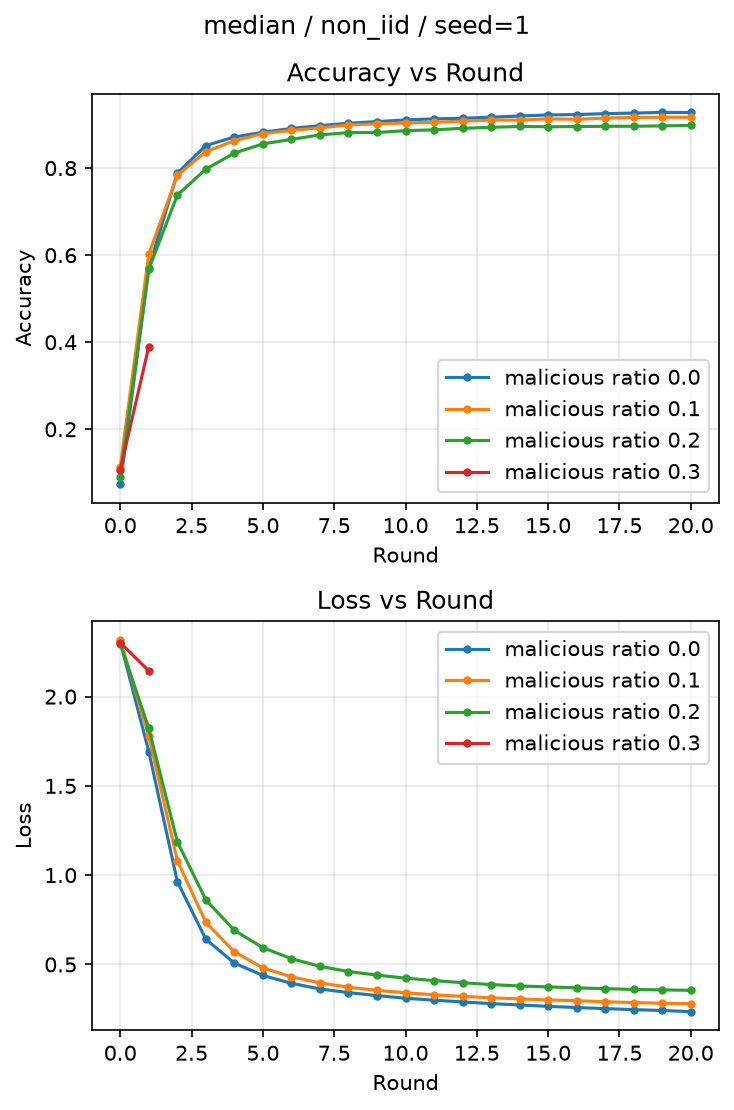
\includegraphics[width=\columnwidth]{median_noniid_seed1_by_ratio.png}
    \caption{Median・Non-IID・Seed 1 における malicious ratio 別の
    Round-Accuracy および Round-Loss の推移（malicious ratio 0.3 は
    Round 0--1 のみ）}
    \label{fig:median_noniid_seed1_by_ratio}
\end{figure}

% =========================================================
\subsubsection{結果}
% =========================================================

図\ref{fig:median_noniid_seed1_by_ratio}に，malicious ratio
0.0, 0.1, 0.2 における Round-Accuracy および Round-Loss の推移を示す．

Median（IID 環境）の場合と同様に，Non-IID 環境においても
malicious ratio の増加に伴って Round 20 時点の Accuracy が
0.9277（ratio 0.0）から 0.9167（ratio 0.1），0.8979（ratio 0.2）と
単調に低下し，Loss も 0.2356 から 0.3553 へ増加する傾向が確認された．
malicious ratio 0.3 については Seed 1 のログが Round 1（Accuracy 0.3900，
Loss 2.1443）で途切れているため本図では傾向を確認できないが，
4.4 節に示した Seed 2・Seed 3 の結果では最終 Accuracy が
約 0.87--0.88 まで低下しており，他の malicious ratio と同様に
比率の増加とともに性能が低下する傾向と整合している．

以上より，Non-IID 環境かつ Seed 1 において，
Median は malicious ratio の増加に対して FedAvg よりも
感度が高く，IID 環境と同様の傾向で攻撃の影響がモデル性能に
現れることが確認された．

\clearpage
% =========================================================
\section{Trimmed Mean（IID環境）における悪性クライアント比率別の評価}
% =========================================================

% =========================================================
\subsection{Trimmed Mean：IID・悪性クライアント比率 0.0}
% =========================================================

\subsubsection{実験条件}

\begin{itemize}
    \item \textbf{Aggregation method:} Trimmed Mean
    \item \textbf{Data split:} IID
    \item \textbf{Malicious ratio:} 0.0
    \item \textbf{Attack:} Adaptive attack
    \item \textbf{Number of rounds:} 20
    \item \textbf{Seeds:} 1, 2, 3
\end{itemize}

% =========================================================
% 実験結果表
% =========================================================

\begin{table}[H]
\centering

\caption{Trimmed Mean（IID，悪性クライアント比率 0.0）における
Accuracy および Loss}

\label{tab:trimmed_mean_iid_ratio0.0}

\footnotesize
\setlength{\tabcolsep}{2.5pt}
\renewcommand{\arraystretch}{0.90}

\resizebox{\columnwidth}{!}{%
\begin{tabular}{c cc cc cc}

\toprule

& \multicolumn{2}{c}{Seed 1}
& \multicolumn{2}{c}{Seed 2}
& \multicolumn{2}{c}{Seed 3} \\

\cmidrule(lr){2-3}
\cmidrule(lr){4-5}
\cmidrule(lr){6-7}

Round
& Acc. & Loss
& Acc. & Loss
& Acc. & Loss \\

\midrule

0 & 0.1001 & 2.3139 & 0.1182 & 2.3078 & 0.0750 & 2.3097 \\
1 & 0.6755 & 1.3224 & -- & -- & 0.7281 & 1.2967 \\
2 & 0.8401 & 0.6540 & -- & -- & 0.8480 & 0.6237 \\
3 & 0.8737 & 0.4924 & -- & -- & 0.8767 & 0.4707 \\
4 & 0.8906 & 0.4170 & -- & -- & 0.8914 & 0.4019 \\
5 & 0.8979 & 0.3725 & -- & -- & 0.8991 & 0.3614 \\
6 & 0.9064 & 0.3434 & -- & -- & 0.9055 & 0.3348 \\
7 & 0.9089 & 0.3225 & -- & -- & 0.9105 & 0.3146 \\
8 & 0.9119 & 0.3073 & -- & -- & 0.9134 & 0.2996 \\
9 & 0.9155 & 0.2920 & -- & -- & 0.9173 & 0.2875 \\
10 & 0.9186 & 0.2807 & -- & -- & 0.9202 & 0.2748 \\
11 & 0.9209 & 0.2708 & -- & -- & 0.9221 & 0.2659 \\
12 & 0.9227 & 0.2608 & -- & -- & 0.9246 & 0.2572 \\
13 & 0.9250 & 0.2534 & -- & -- & 0.9259 & 0.2484 \\
14 & 0.9278 & 0.2468 & -- & -- & 0.9286 & 0.2415 \\
15 & 0.9285 & 0.2390 & -- & -- & 0.9303 & 0.2337 \\
16 & 0.9312 & 0.2316 & -- & -- & 0.9321 & 0.2279 \\
17 & 0.9329 & 0.2246 & -- & -- & 0.9339 & 0.2212 \\
18 & 0.9341 & 0.2201 & -- & -- & 0.9362 & 0.2159 \\
19 & 0.9360 & 0.2142 & -- & -- & 0.9365 & 0.2093 \\
20 & 0.9362 & 0.2094 & -- & -- & 0.9385 & 0.2047 \\

\bottomrule

\end{tabular}%
}

\end{table}
\begin{figure}[H]
    \centering
    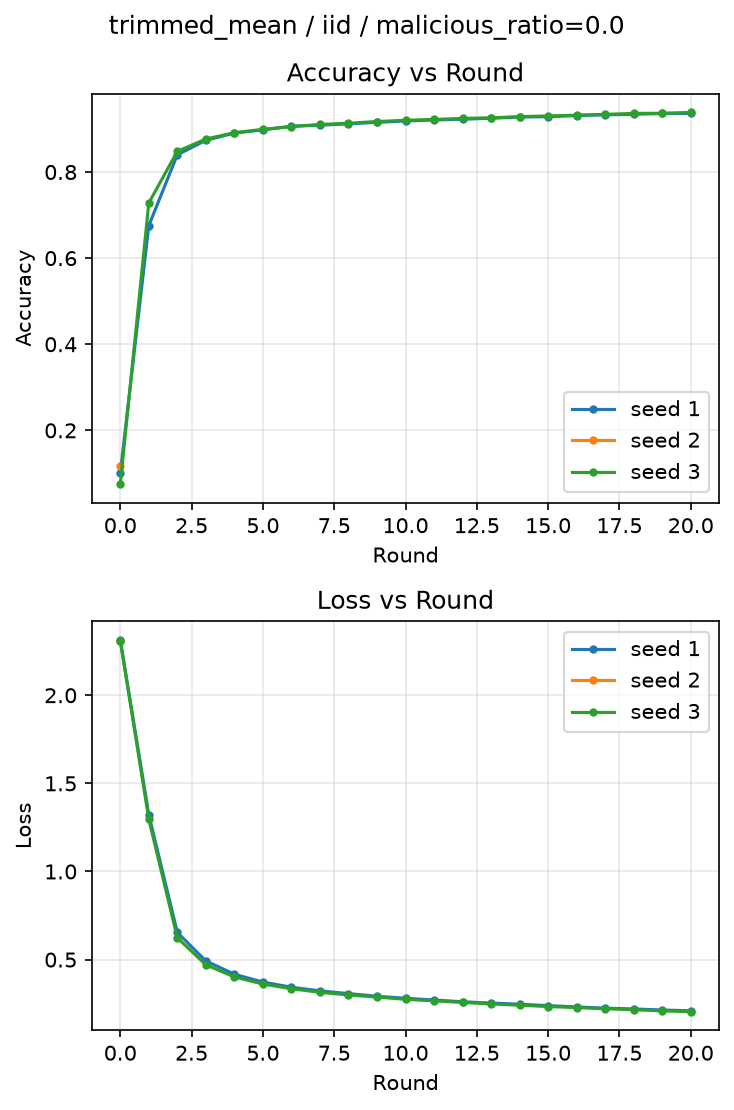
\includegraphics[width=\columnwidth]{seed_curves_trimmed_mean_iid_ratio0.0.png}
    \caption{Seed ごとの Round-Accuracy および Round-Loss の推移（IID，悪性クライアント比率 0.0）}
    \label{fig:seed_curves_trimmed_mean_iid_ratio0.0}
\end{figure}
% =========================================================
\subsubsection{結果}
% =========================================================

表\ref{tab:trimmed_mean_iid_ratio0.0}に，各ラウンドにおける
Accuracy および Loss を示す．

学習開始時（Round 0）の Accuracy は約 0.0750--0.1182 であったが，Round 1 では約 0.6755--0.7281 まで上昇した． その後も学習ラウンドの進行に伴って Accuracy は継続的に向上し，Round 20 ではすべての Seed において約 0.9362--0.9385 に達した． Round 20 時点の Loss は約 0.2047--0.2094 であった．

なお，Seed 2（Round 0 まで） は Round 20 到達前にログが途切れており，実験が途中で終了したものと考えられる（原因不明のため，欠損箇所は表中で「--」と表記した）．

\clearpage
% =========================================================
\subsection{Trimmed Mean：IID・悪性クライアント比率 0.1}
% =========================================================

\subsubsection{実験条件}

\begin{itemize}
    \item \textbf{Aggregation method:} Trimmed Mean
    \item \textbf{Data split:} IID
    \item \textbf{Malicious ratio:} 0.1
    \item \textbf{Attack:} Adaptive attack
    \item \textbf{Number of rounds:} 20
    \item \textbf{Seeds:} 1, 2, 3
\end{itemize}

% =========================================================
% 実験結果表
% =========================================================

\begin{table}[H]
\centering

\caption{Trimmed Mean（IID，悪性クライアント比率 0.1）における
Accuracy および Loss}

\label{tab:trimmed_mean_iid_ratio0.1}

\footnotesize
\setlength{\tabcolsep}{2.5pt}
\renewcommand{\arraystretch}{0.90}

\resizebox{\columnwidth}{!}{%
\begin{tabular}{c cc cc cc}

\toprule

& \multicolumn{2}{c}{Seed 1}
& \multicolumn{2}{c}{Seed 2}
& \multicolumn{2}{c}{Seed 3} \\

\cmidrule(lr){2-3}
\cmidrule(lr){4-5}
\cmidrule(lr){6-7}

Round
& Acc. & Loss
& Acc. & Loss
& Acc. & Loss \\

\midrule

0 & 0.1035 & 2.3091 & 0.0618 & 2.3369 & 0.1074 & 2.3231 \\
1 & 0.7045 & 1.4503 & 0.6472 & 1.5831 & 0.7567 & 1.4969 \\
2 & 0.8401 & 0.6960 & 0.8266 & 0.7694 & 0.8423 & 0.7027 \\
3 & 0.8709 & 0.5201 & 0.8659 & 0.5416 & 0.8731 & 0.5243 \\
4 & 0.8825 & 0.4441 & 0.8819 & 0.4522 & 0.8864 & 0.4461 \\
5 & 0.8905 & 0.4021 & 0.8930 & 0.4013 & 0.8946 & 0.4025 \\
6 & 0.8957 & 0.3738 & 0.8967 & 0.3710 & 0.8975 & 0.3746 \\
7 & 0.9014 & 0.3555 & 0.9017 & 0.3507 & 0.9021 & 0.3546 \\
8 & 0.9032 & 0.3403 & 0.9052 & 0.3346 & 0.9045 & 0.3410 \\
9 & 0.9048 & 0.3292 & 0.9066 & 0.3233 & 0.9057 & 0.3292 \\
10 & 0.9069 & 0.3202 & 0.9092 & 0.3137 & 0.9078 & 0.3201 \\
11 & 0.9082 & 0.3127 & 0.9103 & 0.3052 & 0.9084 & 0.3128 \\
12 & 0.9094 & 0.3048 & 0.9115 & 0.2987 & 0.9117 & 0.3061 \\
13 & 0.9106 & 0.2991 & 0.9130 & 0.2931 & 0.9131 & 0.3005 \\
14 & 0.9135 & 0.2923 & 0.9148 & 0.2874 & 0.9138 & 0.2956 \\
15 & 0.9143 & 0.2875 & 0.9159 & 0.2824 & 0.9154 & 0.2909 \\
16 & 0.9151 & 0.2828 & 0.9170 & 0.2778 & 0.9158 & 0.2867 \\
17 & 0.9160 & 0.2784 & 0.9185 & 0.2734 & 0.9165 & 0.2827 \\
18 & 0.9174 & 0.2743 & 0.9194 & 0.2696 & 0.9177 & 0.2793 \\
19 & 0.9187 & 0.2705 & 0.9196 & 0.2660 & 0.9181 & 0.2758 \\
20 & 0.9199 & 0.2667 & 0.9200 & 0.2624 & 0.9197 & 0.2726 \\

\bottomrule

\end{tabular}%
}

\end{table}
\begin{figure}[H]
    \centering
    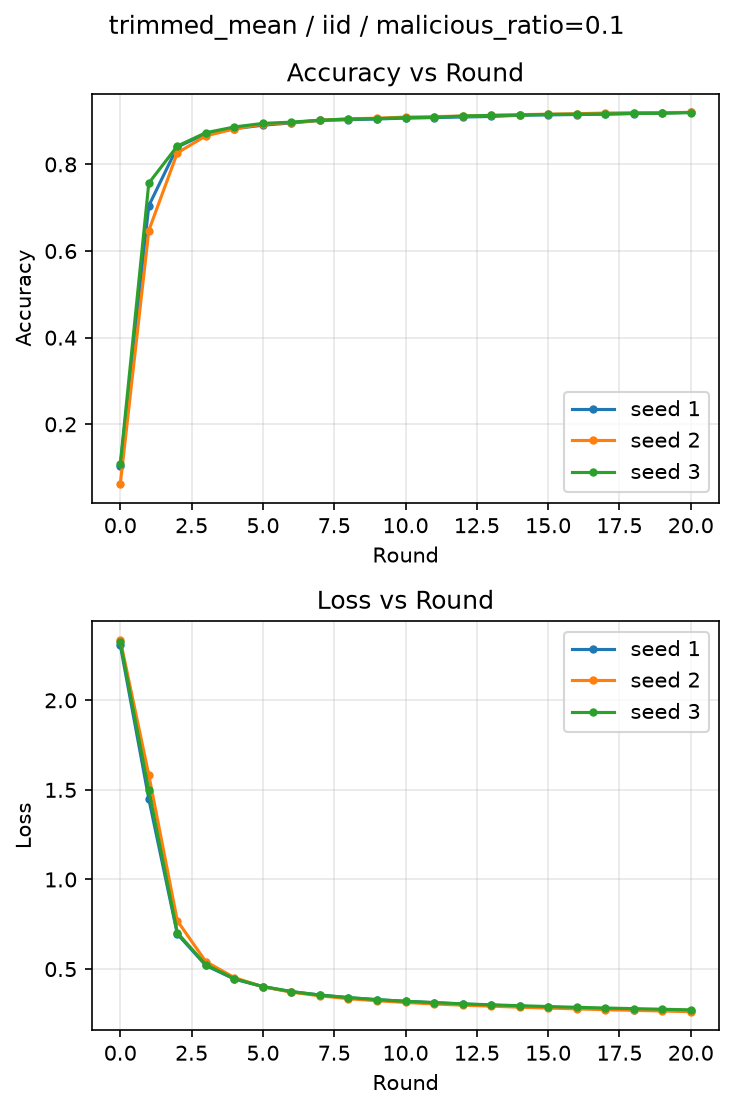
\includegraphics[width=\columnwidth]{seed_curves_trimmed_mean_iid_ratio0.1.png}
    \caption{Seed ごとの Round-Accuracy および Round-Loss の推移（IID，悪性クライアント比率 0.1）}
    \label{fig:seed_curves_trimmed_mean_iid_ratio0.1}
\end{figure}
% =========================================================
\subsubsection{結果}
% =========================================================

表\ref{tab:trimmed_mean_iid_ratio0.1}に，各ラウンドにおける
Accuracy および Loss を示す．

学習開始時（Round 0）の Accuracy は約 0.0618--0.1074 であったが，Round 1 では約 0.6472--0.7567 まで上昇した． その後も学習ラウンドの進行に伴って Accuracy は継続的に向上し，Round 20 ではすべての Seed において約 0.9197--0.9200 に達した． Round 20 時点の Loss は約 0.2624--0.2726 であった． 悪性クライアント比率 0.0 の場合（最終 Accuracy 平均 約 0.9374）と比較しても最終的な Accuracy に大きな差は見られず，本条件下でも学習は概ね安定していたといえる．

\clearpage
% =========================================================
\subsection{Trimmed Mean：IID・悪性クライアント比率 0.2}
% =========================================================

\subsubsection{実験条件}

\begin{itemize}
    \item \textbf{Aggregation method:} Trimmed Mean
    \item \textbf{Data split:} IID
    \item \textbf{Malicious ratio:} 0.2
    \item \textbf{Attack:} Adaptive attack
    \item \textbf{Number of rounds:} 20
    \item \textbf{Seeds:} 1, 2, 3
\end{itemize}

% =========================================================
% 実験結果表
% =========================================================

\begin{table}[H]
\centering

\caption{Trimmed Mean（IID，悪性クライアント比率 0.2）における
Accuracy および Loss}

\label{tab:trimmed_mean_iid_ratio0.2}

\footnotesize
\setlength{\tabcolsep}{2.5pt}
\renewcommand{\arraystretch}{0.90}

\resizebox{\columnwidth}{!}{%
\begin{tabular}{c cc cc cc}

\toprule

& \multicolumn{2}{c}{Seed 1}
& \multicolumn{2}{c}{Seed 2}
& \multicolumn{2}{c}{Seed 3} \\

\cmidrule(lr){2-3}
\cmidrule(lr){4-5}
\cmidrule(lr){6-7}

Round
& Acc. & Loss
& Acc. & Loss
& Acc. & Loss \\

\midrule

0 & 0.1000 & 2.3134 & 0.1030 & 2.3156 & 0.0663 & 2.3159 \\
1 & 0.7132 & 1.6572 & 0.6580 & 1.5943 & 0.6593 & 1.6417 \\
2 & 0.8329 & 0.8039 & 0.8388 & 0.8033 & 0.8098 & 0.8490 \\
3 & 0.8647 & 0.5744 & 0.8691 & 0.5766 & 0.8557 & 0.6115 \\
4 & 0.8788 & 0.4837 & 0.8819 & 0.4868 & 0.8721 & 0.5100 \\
5 & 0.8860 & 0.4384 & 0.8882 & 0.4387 & 0.8813 & 0.4555 \\
6 & 0.8902 & 0.4119 & 0.8917 & 0.4102 & 0.8870 & 0.4244 \\
7 & 0.8938 & 0.3925 & 0.8967 & 0.3920 & 0.8912 & 0.4035 \\
8 & 0.8958 & 0.3803 & 0.8979 & 0.3790 & 0.8940 & 0.3877 \\
9 & 0.8967 & 0.3708 & 0.9000 & 0.3685 & 0.8953 & 0.3766 \\
10 & 0.8982 & 0.3638 & 0.9005 & 0.3598 & 0.8964 & 0.3693 \\
11 & 0.8984 & 0.3576 & 0.9011 & 0.3545 & 0.8982 & 0.3620 \\
12 & 0.8999 & 0.3533 & 0.9024 & 0.3492 & 0.8992 & 0.3566 \\
13 & 0.8998 & 0.3498 & 0.9027 & 0.3456 & 0.9003 & 0.3517 \\
14 & 0.9003 & 0.3465 & 0.9032 & 0.3423 & 0.9014 & 0.3471 \\
15 & 0.9005 & 0.3429 & 0.9038 & 0.3389 & 0.9015 & 0.3440 \\
16 & 0.9019 & 0.3403 & 0.9045 & 0.3363 & 0.9028 & 0.3403 \\
17 & 0.9025 & 0.3366 & 0.9041 & 0.3350 & 0.9039 & 0.3374 \\
18 & 0.9026 & 0.3348 & 0.9045 & 0.3322 & 0.9038 & 0.3361 \\
19 & 0.9037 & 0.3325 & 0.9055 & 0.3305 & 0.9044 & 0.3330 \\
20 & 0.9037 & 0.3309 & 0.9061 & 0.3283 & 0.9038 & 0.3311 \\

\bottomrule

\end{tabular}%
}

\end{table}
\begin{figure}[H]
    \centering
    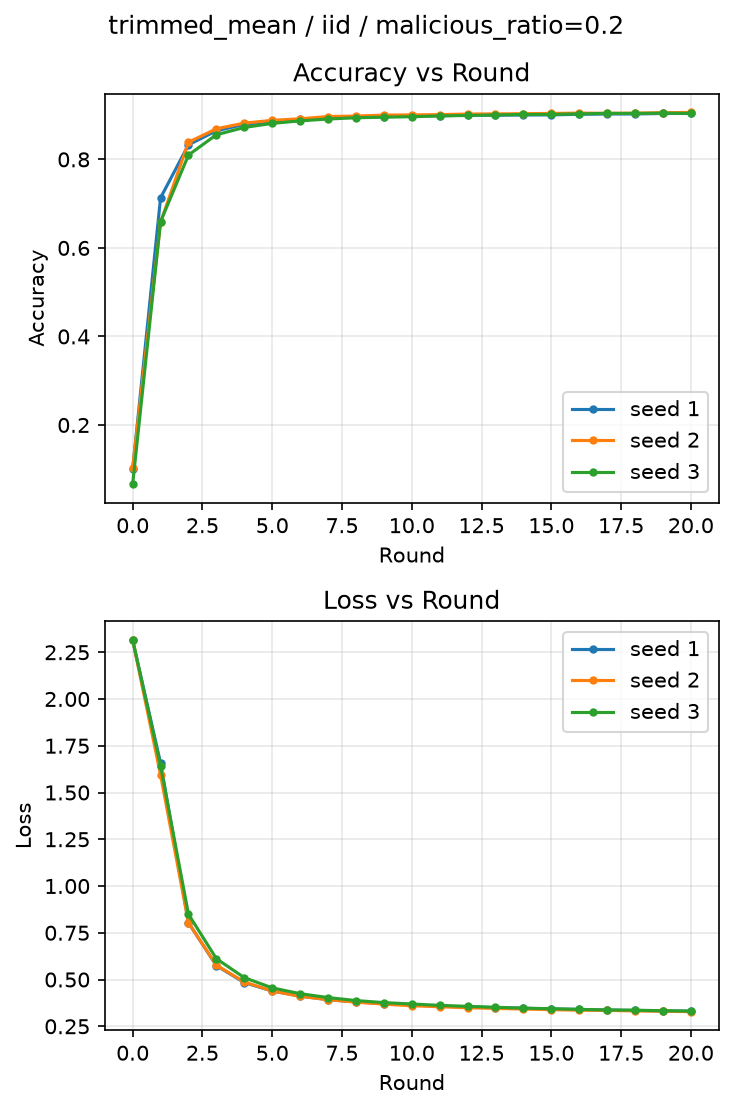
\includegraphics[width=\columnwidth]{seed_curves_trimmed_mean_iid_ratio0.2.png}
    \caption{Seed ごとの Round-Accuracy および Round-Loss の推移（IID，悪性クライアント比率 0.2）}
    \label{fig:seed_curves_trimmed_mean_iid_ratio0.2}
\end{figure}
% =========================================================
\subsubsection{結果}
% =========================================================

表\ref{tab:trimmed_mean_iid_ratio0.2}に，各ラウンドにおける
Accuracy および Loss を示す．

学習開始時（Round 0）の Accuracy は約 0.0663--0.1030 であったが，Round 1 では約 0.6580--0.7132 まで上昇した． その後も学習ラウンドの進行に伴って Accuracy は継続的に向上し，Round 20 ではすべての Seed において約 0.9037--0.9061 に達した． Round 20 時点の Loss は約 0.3283--0.3311 であった． 悪性クライアント比率 0.0 の場合（最終 Accuracy 平均 約 0.9374）と比較すると，本条件では約 0.0328 ポイント低い水準にとどまっており，悪性クライアント比率 0.2 における攻撃の影響が最終的な Accuracy にも現れていることが分かる．

\clearpage
% =========================================================
\subsection{Trimmed Mean：IID・悪性クライアント比率 0.3}
% =========================================================

\subsubsection{実験条件}

\begin{itemize}
    \item \textbf{Aggregation method:} Trimmed Mean
    \item \textbf{Data split:} IID
    \item \textbf{Malicious ratio:} 0.3
    \item \textbf{Attack:} Adaptive attack
    \item \textbf{Number of rounds:} 20
    \item \textbf{Seeds:} 1, 2, 3
\end{itemize}

% =========================================================
% 実験結果表
% =========================================================

\begin{table}[H]
\centering

\caption{Trimmed Mean（IID，悪性クライアント比率 0.3）における
Accuracy および Loss}

\label{tab:trimmed_mean_iid_ratio0.3}

\footnotesize
\setlength{\tabcolsep}{2.5pt}
\renewcommand{\arraystretch}{0.90}

\resizebox{\columnwidth}{!}{%
\begin{tabular}{c cc cc cc}

\toprule

& \multicolumn{2}{c}{Seed 1}
& \multicolumn{2}{c}{Seed 2}
& \multicolumn{2}{c}{Seed 3} \\

\cmidrule(lr){2-3}
\cmidrule(lr){4-5}
\cmidrule(lr){6-7}

Round
& Acc. & Loss
& Acc. & Loss
& Acc. & Loss \\

\midrule

0 & 0.0397 & 2.3338 & 0.0989 & 2.3039 & 0.1016 & 2.3256 \\
1 & 0.6609 & 1.6953 & 0.6109 & 1.7661 & 0.6324 & 1.9566 \\
2 & 0.7797 & 0.9695 & 0.7704 & 1.0044 & 0.7845 & 1.1248 \\
3 & 0.8322 & 0.7233 & 0.8446 & 0.7035 & 0.8430 & 0.7382 \\
4 & 0.8548 & 0.6096 & 0.8651 & 0.5858 & 0.8626 & 0.5952 \\
5 & 0.8680 & 0.5465 & 0.8737 & 0.5304 & 0.8703 & 0.5321 \\
6 & 0.8741 & 0.5086 & 0.8781 & 0.4955 & 0.8756 & 0.4981 \\
7 & 0.8762 & 0.4860 & 0.8827 & 0.4748 & 0.8781 & 0.4780 \\
8 & 0.8798 & 0.4690 & 0.8860 & 0.4605 & 0.8798 & 0.4661 \\
9 & 0.8823 & 0.4583 & 0.8864 & 0.4503 & 0.8801 & 0.4576 \\
10 & 0.8822 & 0.4490 & 0.8863 & 0.4441 & 0.8804 & 0.4506 \\
11 & 0.8829 & 0.4428 & 0.8883 & 0.4393 & 0.8818 & 0.4462 \\
12 & 0.8837 & 0.4378 & 0.8877 & 0.4356 & 0.8831 & 0.4391 \\
13 & 0.8840 & 0.4341 & 0.8881 & 0.4330 & 0.8830 & 0.4374 \\
14 & 0.8848 & 0.4310 & 0.8885 & 0.4306 & 0.8819 & 0.4379 \\
15 & 0.8851 & 0.4284 & 0.8883 & 0.4295 & 0.8816 & 0.4349 \\
16 & 0.8859 & 0.4255 & 0.8893 & 0.4296 & 0.8826 & 0.4317 \\
17 & 0.8857 & 0.4249 & 0.8892 & 0.4278 & 0.8819 & 0.4320 \\
18 & 0.8845 & 0.4223 & 0.8885 & 0.4295 & 0.8831 & 0.4301 \\
19 & 0.8860 & 0.4212 & 0.8892 & 0.4263 & 0.8817 & 0.4309 \\
20 & 0.8866 & 0.4197 & 0.8889 & 0.4258 & 0.8808 & 0.4310 \\

\bottomrule

\end{tabular}%
}

\end{table}
\begin{figure}[H]
    \centering
    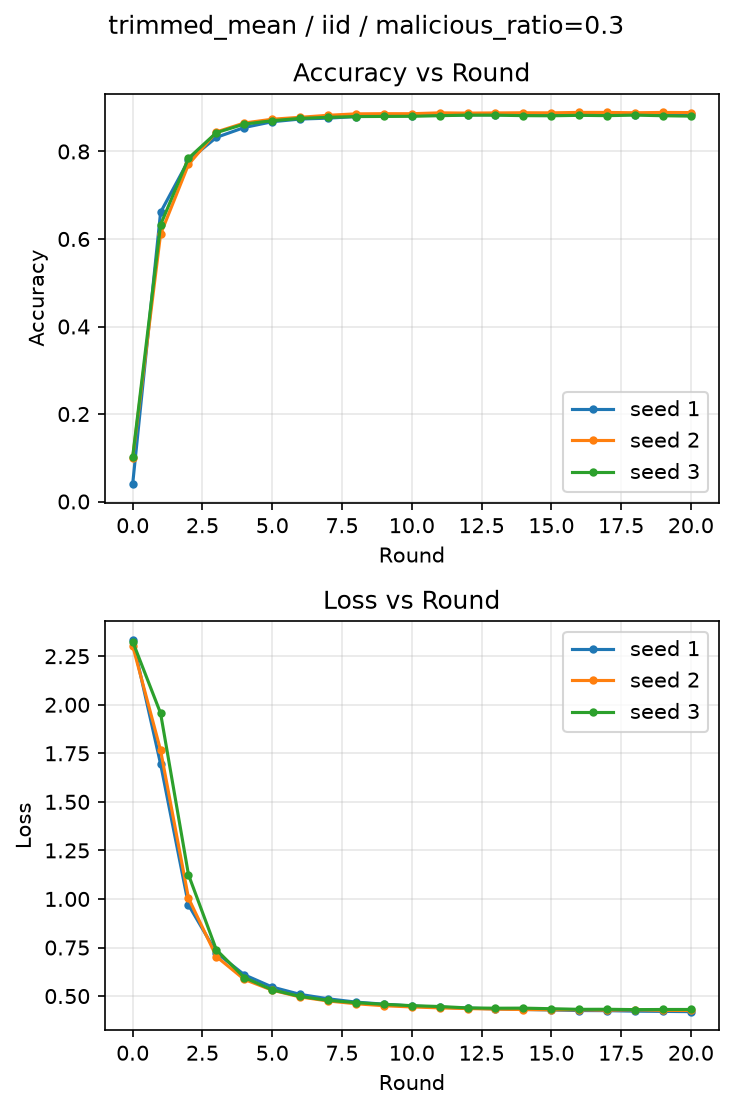
\includegraphics[width=\columnwidth]{seed_curves_trimmed_mean_iid_ratio0.3.png}
    \caption{Seed ごとの Round-Accuracy および Round-Loss の推移（IID，悪性クライアント比率 0.3）}
    \label{fig:seed_curves_trimmed_mean_iid_ratio0.3}
\end{figure}
% =========================================================
\subsubsection{結果}
% =========================================================

表\ref{tab:trimmed_mean_iid_ratio0.3}に，各ラウンドにおける
Accuracy および Loss を示す．

学習開始時（Round 0）の Accuracy は約 0.0397--0.1016 であったが，Round 1 では約 0.6109--0.6609 まで上昇した． その後も学習ラウンドの進行に伴って Accuracy は継続的に向上し，Round 20 ではすべての Seed において約 0.8808--0.8889 に達した． Round 20 時点の Loss は約 0.4197--0.4310 であった． 悪性クライアント比率 0.0 の場合（最終 Accuracy 平均 約 0.9374）と比較すると，本条件では約 0.0519 ポイント低い水準にとどまっており，悪性クライアント比率 0.3 における攻撃の影響が最終的な Accuracy にも現れていることが分かる．

\clearpage
% =========================================================
\subsection{Trimmed Mean：IID・悪性クライアント比率別の比較（Seed 1）}
% =========================================================

\subsubsection{実験条件}

\begin{itemize}
    \item \textbf{Aggregation method:} Trimmed Mean
    \item \textbf{Data split:} IID
    \item \textbf{Malicious ratio:} 0.0, 0.1, 0.2, 0.3
    \item \textbf{Attack:} Adaptive attack
    \item \textbf{Number of rounds:} 20
    \item \textbf{Seed:} 1
\end{itemize}

5.1--5.4 節で示した Seed 1 の結果を malicious ratio 別に
1つの図上で比較できるよう再構成した．
図の作成には \verb|result/plot_fedavg_iid_seed1_by_ratio.py| を
\verb|--aggregation trimmed_mean| オプションで用い，
\verb|result/results.csv| から Trimmed Mean・IID・seed=1 の条件に一致する
run を malicious ratio ごとに抽出して描画した．

% =========================================================
% 実験結果図
% =========================================================

\begin{figure}[H]
    \centering
    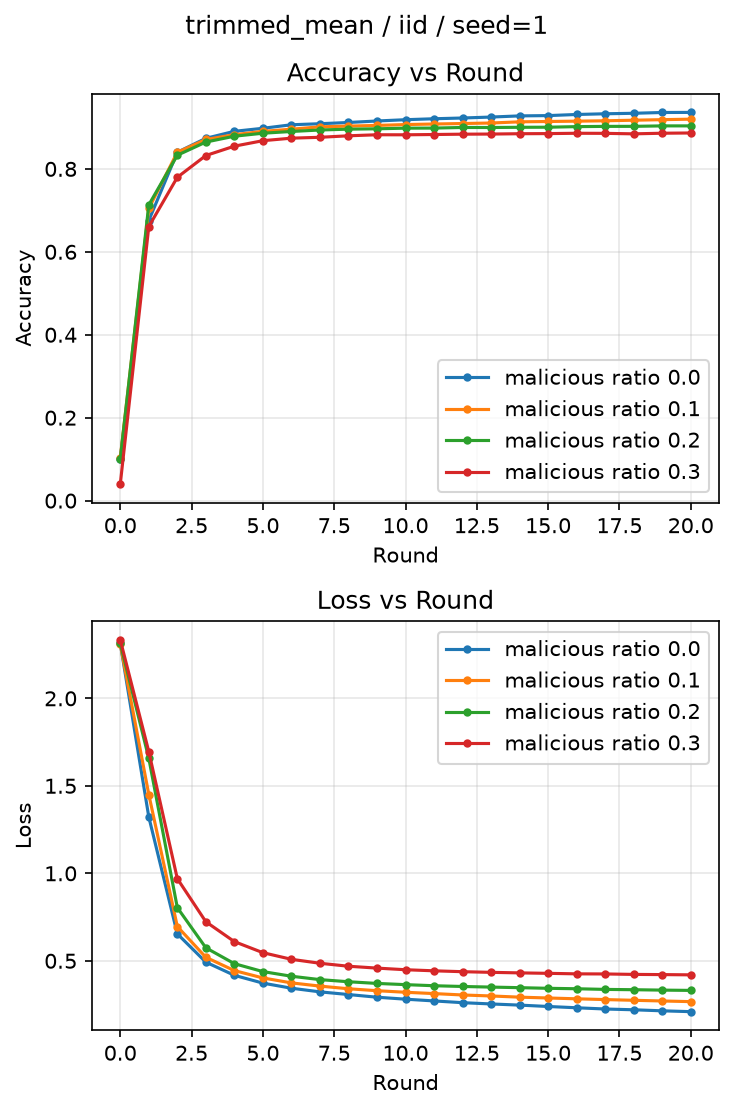
\includegraphics[width=\columnwidth]{trimmed_mean_iid_seed1_by_ratio.png}
    \caption{Trimmed Mean・IID・Seed 1 における malicious ratio 別の
    Round-Accuracy および Round-Loss の推移}
    \label{fig:trimmed_mean_iid_seed1_by_ratio}
\end{figure}

% =========================================================
\subsubsection{結果}
% =========================================================

図\ref{fig:trimmed_mean_iid_seed1_by_ratio}に，malicious ratio
0.0, 0.1, 0.2, 0.3 における Round-Accuracy および Round-Loss の推移を示す．

Median の場合と同様に，Trimmed Mean でも malicious ratio の増加に伴って
Round 20 時点の Accuracy が 0.9362（ratio 0.0）から
0.9199（ratio 0.1），0.9037（ratio 0.2），0.8866（ratio 0.3）と
単調に低下する傾向が確認された．
Loss についても同様に，Round 20 時点で 0.2094（ratio 0.0）から
0.4197（ratio 0.3）まで malicious ratio の増加とともに増加しており，
malicious ratio 0.3 における Loss の増加幅は Median（0.2073 から 0.3777）
よりもやや大きい．

以上より，IID 環境かつ Seed 1 において，
Trimmed Mean は Median と同様に malicious ratio の増加に対して
FedAvg よりも感度が高く，攻撃の影響がモデル性能に明確に
現れることが確認された．

\clearpage
% =========================================================
\section{Trimmed Mean（Non-IID環境）における悪性クライアント比率別の評価}
% =========================================================

% =========================================================
\subsection{Trimmed Mean：Non-IID・悪性クライアント比率 0.0}
% =========================================================

\subsubsection{実験条件}

\begin{itemize}
    \item \textbf{Aggregation method:} Trimmed Mean
    \item \textbf{Data split:} Non-IID
    \item \textbf{Malicious ratio:} 0.0
    \item \textbf{Attack:} Adaptive attack
    \item \textbf{Number of rounds:} 20
    \item \textbf{Seeds:} 1, 2, 3
\end{itemize}

% =========================================================
% 実験結果表
% =========================================================

\begin{table}[H]
\centering

\caption{Trimmed Mean（Non-IID，悪性クライアント比率 0.0）における
Accuracy および Loss}

\label{tab:trimmed_mean_non_iid_ratio0.0}

\footnotesize
\setlength{\tabcolsep}{2.5pt}
\renewcommand{\arraystretch}{0.90}

\resizebox{\columnwidth}{!}{%
\begin{tabular}{c cc cc cc}

\toprule

& \multicolumn{2}{c}{Seed 1}
& \multicolumn{2}{c}{Seed 2}
& \multicolumn{2}{c}{Seed 3} \\

\cmidrule(lr){2-3}
\cmidrule(lr){4-5}
\cmidrule(lr){6-7}

Round
& Acc. & Loss
& Acc. & Loss
& Acc. & Loss \\

\midrule

0 & 0.0858 & 2.3095 & 0.0841 & 2.3143 & 0.1066 & 2.3146 \\
1 & 0.5908 & 1.6895 & 0.6859 & 1.7587 & 0.6340 & 1.6930 \\
2 & 0.8134 & 0.9609 & 0.7749 & 0.9941 & 0.7684 & 0.9580 \\
3 & 0.8624 & 0.6391 & 0.8471 & 0.6681 & 0.8505 & 0.6285 \\
4 & 0.8821 & 0.5041 & 0.8748 & 0.5183 & 0.8727 & 0.4931 \\
5 & 0.8925 & 0.4312 & 0.8861 & 0.4411 & 0.8839 & 0.4259 \\
6 & 0.8998 & 0.3886 & 0.8949 & 0.3952 & 0.8940 & 0.3832 \\
7 & 0.9048 & 0.3586 & 0.8999 & 0.3652 & 0.8968 & 0.3547 \\
8 & 0.9084 & 0.3362 & 0.9037 & 0.3439 & 0.9026 & 0.3328 \\
9 & 0.9115 & 0.3181 & 0.9075 & 0.3266 & 0.9056 & 0.3167 \\
10 & 0.9146 & 0.3037 & 0.9107 & 0.3124 & 0.9077 & 0.3051 \\
11 & 0.9160 & 0.2942 & 0.9122 & 0.3037 & 0.9101 & 0.2933 \\
12 & 0.9186 & 0.2824 & 0.9155 & 0.2908 & 0.9162 & 0.2822 \\
13 & 0.9201 & 0.2739 & 0.9168 & 0.2809 & 0.9169 & 0.2738 \\
14 & 0.9225 & 0.2663 & 0.9189 & 0.2728 & 0.9189 & 0.2673 \\
15 & 0.9246 & 0.2585 & 0.9207 & 0.2669 & 0.9206 & 0.2591 \\
16 & 0.9260 & 0.2511 & 0.9232 & 0.2575 & 0.9224 & 0.2516 \\
17 & 0.9275 & 0.2445 & 0.9239 & 0.2524 & 0.9257 & 0.2448 \\
18 & 0.9289 & 0.2390 & 0.9254 & 0.2473 & 0.9272 & 0.2399 \\
19 & 0.9300 & 0.2330 & 0.9275 & 0.2401 & 0.9292 & 0.2331 \\
20 & 0.9307 & 0.2277 & 0.9290 & 0.2350 & 0.9305 & 0.2280 \\

\bottomrule

\end{tabular}%
}

\end{table}
\begin{figure}[H]
    \centering
    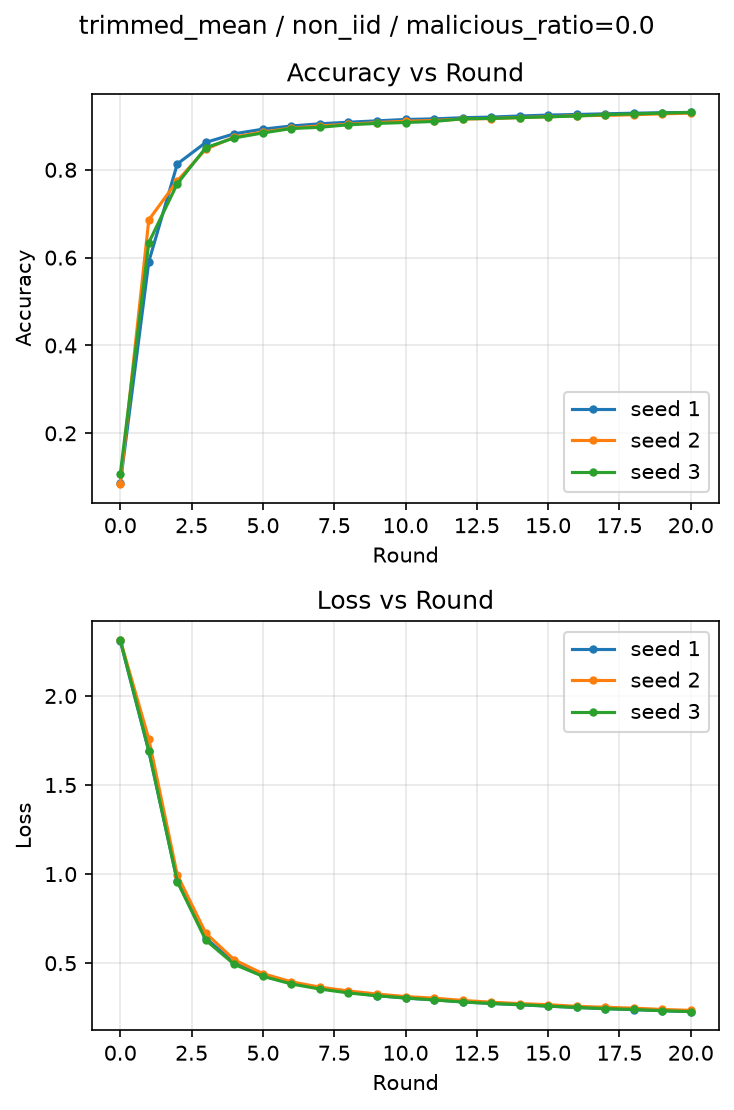
\includegraphics[width=\columnwidth]{seed_curves_trimmed_mean_non_iid_ratio0.0.png}
    \caption{Seed ごとの Round-Accuracy および Round-Loss の推移（Non-IID，悪性クライアント比率 0.0）}
    \label{fig:seed_curves_trimmed_mean_non_iid_ratio0.0}
\end{figure}
% =========================================================
\subsubsection{結果}
% =========================================================

表\ref{tab:trimmed_mean_non_iid_ratio0.0}に，各ラウンドにおける
Accuracy および Loss を示す．

学習開始時（Round 0）の Accuracy は約 0.0841--0.1066 であったが，Round 1 では約 0.5908--0.6859 まで上昇した． その後も学習ラウンドの進行に伴って Accuracy は継続的に向上し，Round 20 ではすべての Seed において約 0.9290--0.9307 に達した． Round 20 時点の Loss は約 0.2277--0.2350 であった．

\clearpage
% =========================================================
\subsection{Trimmed Mean：Non-IID・悪性クライアント比率 0.1}
% =========================================================

\subsubsection{実験条件}

\begin{itemize}
    \item \textbf{Aggregation method:} Trimmed Mean
    \item \textbf{Data split:} Non-IID
    \item \textbf{Malicious ratio:} 0.1
    \item \textbf{Attack:} Adaptive attack
    \item \textbf{Number of rounds:} 20
    \item \textbf{Seeds:} 1, 2, 3
\end{itemize}

% =========================================================
% 実験結果表
% =========================================================

\begin{table}[H]
\centering

\caption{Trimmed Mean（Non-IID，悪性クライアント比率 0.1）における
Accuracy および Loss}

\label{tab:trimmed_mean_non_iid_ratio0.1}

\footnotesize
\setlength{\tabcolsep}{2.5pt}
\renewcommand{\arraystretch}{0.90}

\resizebox{\columnwidth}{!}{%
\begin{tabular}{c cc cc cc}

\toprule

& \multicolumn{2}{c}{Seed 1}
& \multicolumn{2}{c}{Seed 2}
& \multicolumn{2}{c}{Seed 3} \\

\cmidrule(lr){2-3}
\cmidrule(lr){4-5}
\cmidrule(lr){6-7}

Round
& Acc. & Loss
& Acc. & Loss
& Acc. & Loss \\

\midrule

0 & 0.1333 & 2.3078 & 0.1321 & 2.2937 & 0.0980 & 2.3173 \\
1 & 0.6716 & 1.7851 & 0.5394 & 1.8575 & 0.6840 & 1.8349 \\
2 & 0.7695 & 1.1007 & 0.7576 & 1.2133 & 0.7879 & 1.1503 \\
3 & 0.8328 & 0.7517 & 0.8203 & 0.8271 & 0.8382 & 0.7776 \\
4 & 0.8574 & 0.5923 & 0.8590 & 0.6427 & 0.8612 & 0.6027 \\
5 & 0.8722 & 0.5095 & 0.8736 & 0.5474 & 0.8765 & 0.5071 \\
6 & 0.8794 & 0.4580 & 0.8814 & 0.4896 & 0.8844 & 0.4517 \\
7 & 0.8865 & 0.4236 & 0.8894 & 0.4489 & 0.8914 & 0.4155 \\
8 & 0.8908 & 0.3987 & 0.8927 & 0.4195 & 0.8954 & 0.3904 \\
9 & 0.8949 & 0.3788 & 0.8965 & 0.3974 & 0.8981 & 0.3720 \\
10 & 0.8977 & 0.3640 & 0.8996 & 0.3809 & 0.9009 & 0.3585 \\
11 & 0.9007 & 0.3522 & 0.9015 & 0.3676 & 0.9018 & 0.3465 \\
12 & 0.9015 & 0.3428 & 0.9036 & 0.3561 & 0.9031 & 0.3378 \\
13 & 0.9034 & 0.3337 & 0.9048 & 0.3461 & 0.9057 & 0.3291 \\
14 & 0.9048 & 0.3257 & 0.9068 & 0.3383 & 0.9076 & 0.3227 \\
15 & 0.9063 & 0.3193 & 0.9090 & 0.3311 & 0.9086 & 0.3163 \\
16 & 0.9078 & 0.3139 & 0.9097 & 0.3246 & 0.9104 & 0.3109 \\
17 & 0.9090 & 0.3087 & 0.9098 & 0.3196 & 0.9118 & 0.3064 \\
18 & 0.9102 & 0.3041 & 0.9117 & 0.3139 & 0.9129 & 0.3021 \\
19 & 0.9115 & 0.2995 & 0.9122 & 0.3093 & 0.9126 & 0.2982 \\
20 & 0.9121 & 0.2959 & 0.9115 & 0.3061 & 0.9139 & 0.2946 \\

\bottomrule

\end{tabular}%
}

\end{table}
\begin{figure}[H]
    \centering
    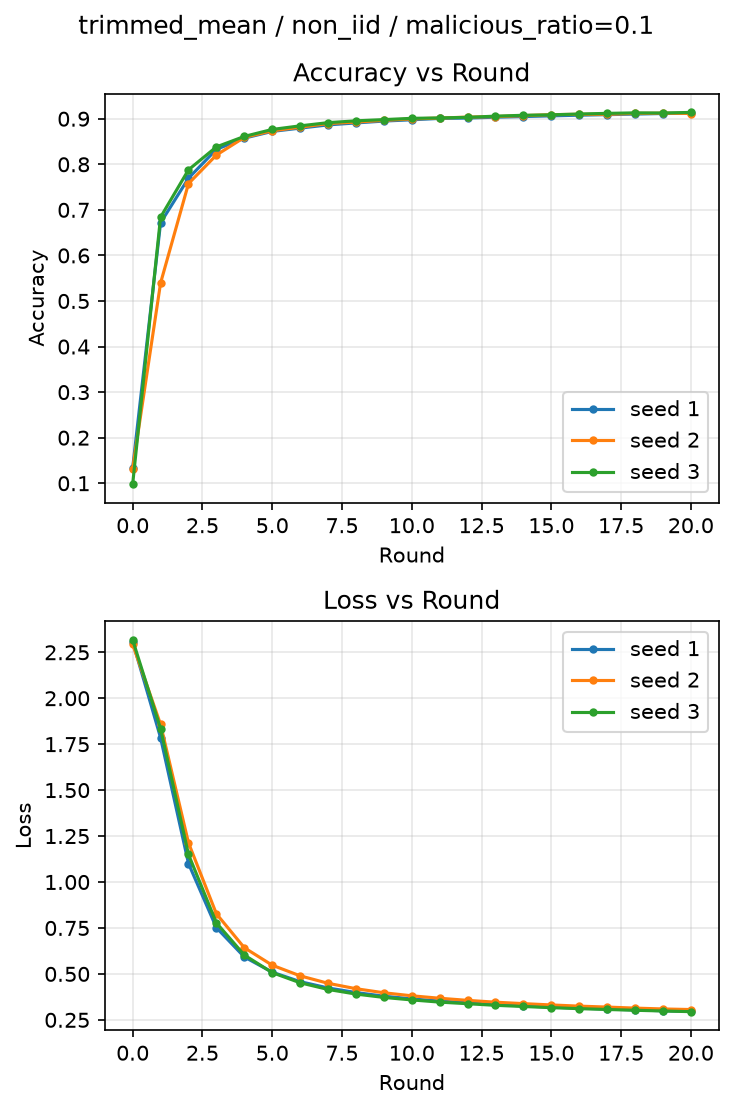
\includegraphics[width=\columnwidth]{seed_curves_trimmed_mean_non_iid_ratio0.1.png}
    \caption{Seed ごとの Round-Accuracy および Round-Loss の推移（Non-IID，悪性クライアント比率 0.1）}
    \label{fig:seed_curves_trimmed_mean_non_iid_ratio0.1}
\end{figure}
% =========================================================
\subsubsection{結果}
% =========================================================

表\ref{tab:trimmed_mean_non_iid_ratio0.1}に，各ラウンドにおける
Accuracy および Loss を示す．

学習開始時（Round 0）の Accuracy は約 0.0980--0.1333 であったが，Round 1 では約 0.5394--0.6840 まで上昇した． その後も学習ラウンドの進行に伴って Accuracy は継続的に向上し，Round 20 ではすべての Seed において約 0.9115--0.9139 に達した． Round 20 時点の Loss は約 0.2946--0.3061 であった． 悪性クライアント比率 0.0 の場合（最終 Accuracy 平均 約 0.9301）と比較しても最終的な Accuracy に大きな差は見られず，本条件下でも学習は概ね安定していたといえる．

\clearpage
% =========================================================
\subsection{Trimmed Mean：Non-IID・悪性クライアント比率 0.2}
% =========================================================

\subsubsection{実験条件}

\begin{itemize}
    \item \textbf{Aggregation method:} Trimmed Mean
    \item \textbf{Data split:} Non-IID
    \item \textbf{Malicious ratio:} 0.2
    \item \textbf{Attack:} Adaptive attack
    \item \textbf{Number of rounds:} 20
    \item \textbf{Seeds:} 1, 2, 3
\end{itemize}

% =========================================================
% 実験結果表
% =========================================================

\begin{table}[H]
\centering

\caption{Trimmed Mean（Non-IID，悪性クライアント比率 0.2）における
Accuracy および Loss}

\label{tab:trimmed_mean_non_iid_ratio0.2}

\footnotesize
\setlength{\tabcolsep}{2.5pt}
\renewcommand{\arraystretch}{0.90}

\resizebox{\columnwidth}{!}{%
\begin{tabular}{c cc cc cc}

\toprule

& \multicolumn{2}{c}{Seed 1}
& \multicolumn{2}{c}{Seed 2}
& \multicolumn{2}{c}{Seed 3} \\

\cmidrule(lr){2-3}
\cmidrule(lr){4-5}
\cmidrule(lr){6-7}

Round
& Acc. & Loss
& Acc. & Loss
& Acc. & Loss \\

\midrule

0 & 0.0945 & 2.3018 & 0.1028 & 2.3038 & 0.1035 & 2.2992 \\
1 & 0.5248 & 1.9902 & 0.6223 & 2.0045 & 0.5495 & 2.0479 \\
2 & 0.7404 & 1.4224 & 0.7337 & 1.4871 & 0.7230 & 1.6053 \\
3 & 0.7963 & 1.0373 & 0.7924 & 1.0935 & 0.8019 & 1.1942 \\
4 & 0.8192 & 0.8259 & 0.8308 & 0.8510 & 0.8369 & 0.9141 \\
5 & 0.8396 & 0.7117 & 0.8480 & 0.7123 & 0.8543 & 0.7437 \\
6 & 0.8478 & 0.6399 & 0.8650 & 0.6267 & 0.8639 & 0.6452 \\
7 & 0.8598 & 0.5893 & 0.8700 & 0.5713 & 0.8714 & 0.5826 \\
8 & 0.8676 & 0.5521 & 0.8751 & 0.5339 & 0.8750 & 0.5411 \\
9 & 0.8723 & 0.5255 & 0.8798 & 0.5061 & 0.8780 & 0.5121 \\
10 & 0.8772 & 0.5047 & 0.8814 & 0.4847 & 0.8806 & 0.4898 \\
11 & 0.8812 & 0.4881 & 0.8843 & 0.4676 & 0.8833 & 0.4735 \\
12 & 0.8826 & 0.4733 & 0.8875 & 0.4537 & 0.8851 & 0.4590 \\
13 & 0.8852 & 0.4625 & 0.8880 & 0.4455 & 0.8860 & 0.4495 \\
14 & 0.8856 & 0.4532 & 0.8878 & 0.4361 & 0.8867 & 0.4403 \\
15 & 0.8882 & 0.4453 & 0.8877 & 0.4315 & 0.8850 & 0.4354 \\
16 & 0.8896 & 0.4381 & 0.8885 & 0.4247 & 0.8858 & 0.4295 \\
17 & 0.8897 & 0.4326 & 0.8881 & 0.4188 & 0.8879 & 0.4241 \\
18 & 0.8907 & 0.4275 & 0.8910 & 0.4125 & 0.8891 & 0.4189 \\
19 & 0.8911 & 0.4239 & 0.8916 & 0.4085 & 0.8892 & 0.4149 \\
20 & 0.8916 & 0.4202 & 0.8924 & 0.4038 & 0.8890 & 0.4112 \\

\bottomrule

\end{tabular}%
}

\end{table}
\begin{figure}[H]
    \centering
    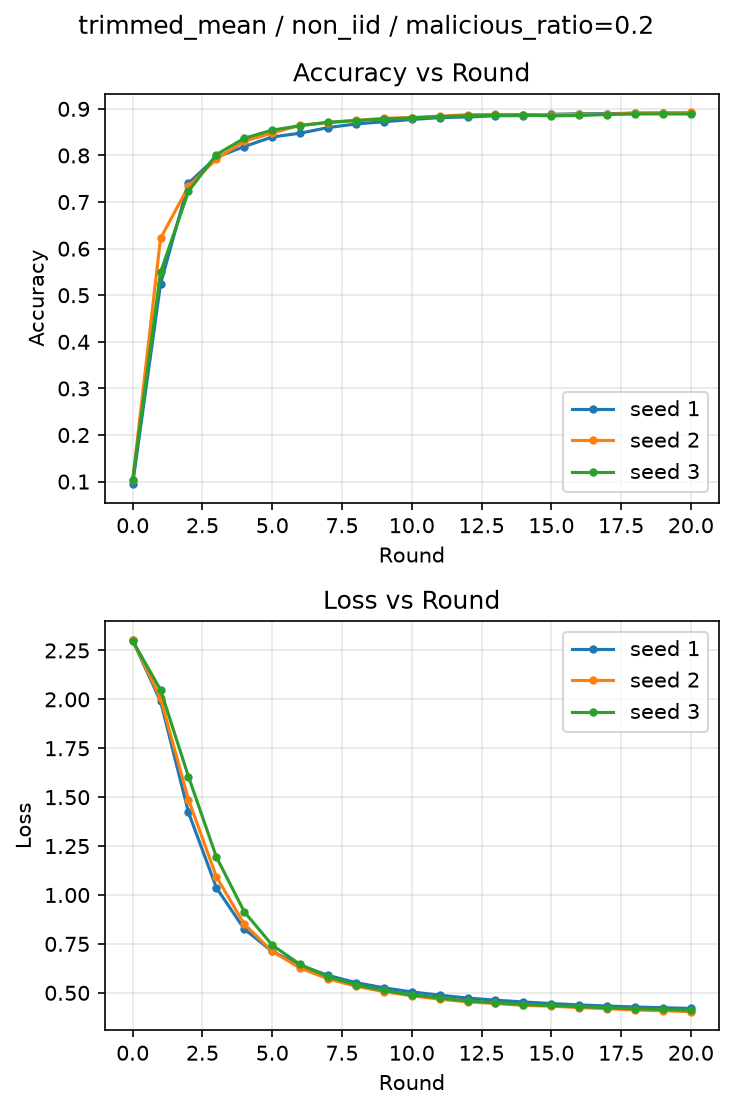
\includegraphics[width=\columnwidth]{seed_curves_trimmed_mean_non_iid_ratio0.2.png}
    \caption{Seed ごとの Round-Accuracy および Round-Loss の推移（Non-IID，悪性クライアント比率 0.2）}
    \label{fig:seed_curves_trimmed_mean_non_iid_ratio0.2}
\end{figure}
% =========================================================
\subsubsection{結果}
% =========================================================

表\ref{tab:trimmed_mean_non_iid_ratio0.2}に，各ラウンドにおける
Accuracy および Loss を示す．

学習開始時（Round 0）の Accuracy は約 0.0945--0.1035 であったが，Round 1 では約 0.5248--0.6223 まで上昇した． その後も学習ラウンドの進行に伴って Accuracy は継続的に向上し，Round 20 ではすべての Seed において約 0.8890--0.8924 に達した． Round 20 時点の Loss は約 0.4038--0.4202 であった． 悪性クライアント比率 0.0 の場合（最終 Accuracy 平均 約 0.9301）と比較すると，本条件では約 0.0391 ポイント低い水準にとどまっており，悪性クライアント比率 0.2 における攻撃の影響が最終的な Accuracy にも現れていることが分かる．

\clearpage
% =========================================================
\subsection{Trimmed Mean：Non-IID・悪性クライアント比率 0.3}
% =========================================================

\subsubsection{実験条件}

\begin{itemize}
    \item \textbf{Aggregation method:} Trimmed Mean
    \item \textbf{Data split:} Non-IID
    \item \textbf{Malicious ratio:} 0.3
    \item \textbf{Attack:} Adaptive attack
    \item \textbf{Number of rounds:} 20
    \item \textbf{Seeds:} 1, 2, 3
\end{itemize}

% =========================================================
% 実験結果表
% =========================================================

\begin{table}[H]
\centering

\caption{Trimmed Mean（Non-IID，悪性クライアント比率 0.3）における
Accuracy および Loss}

\label{tab:trimmed_mean_non_iid_ratio0.3}

\footnotesize
\setlength{\tabcolsep}{2.5pt}
\renewcommand{\arraystretch}{0.90}

\resizebox{\columnwidth}{!}{%
\begin{tabular}{c cc cc cc}

\toprule

& \multicolumn{2}{c}{Seed 1}
& \multicolumn{2}{c}{Seed 2}
& \multicolumn{2}{c}{Seed 3} \\

\cmidrule(lr){2-3}
\cmidrule(lr){4-5}
\cmidrule(lr){6-7}

Round
& Acc. & Loss
& Acc. & Loss
& Acc. & Loss \\

\midrule

0 & 0.1125 & 2.3052 & 0.1099 & 2.3151 & 0.1010 & 2.3104 \\
1 & 0.2194 & 2.2402 & 0.2862 & 2.2320 & 0.2291 & 2.1961 \\
2 & 0.5315 & 2.0940 & 0.4496 & 2.0340 & 0.4603 & 1.9332 \\
3 & 0.5530 & 1.8956 & 0.5868 & 1.7690 & 0.5746 & 1.6428 \\
4 & 0.5974 & 1.7008 & 0.7081 & 1.5119 & 0.6652 & 1.4068 \\
5 & 0.6196 & 1.5251 & 0.7538 & 1.2995 & 0.6988 & 1.2258 \\
6 & 0.6460 & 1.3673 & 0.7812 & 1.1352 & 0.7352 & 1.0895 \\
7 & 0.6600 & 1.2454 & 0.8008 & 1.0175 & 0.7595 & 0.9895 \\
8 & 0.6682 & 1.1516 & 0.8049 & 0.9239 & 0.7851 & 0.9107 \\
9 & 0.6770 & 1.0787 & 0.8101 & 0.8582 & 0.8017 & 0.8500 \\
10 & 0.6888 & 1.0200 & 0.8184 & 0.8101 & 0.8174 & 0.8044 \\
11 & 0.6971 & 0.9759 & 0.8177 & 0.7754 & 0.8198 & 0.7719 \\
12 & 0.7078 & 0.9455 & 0.8215 & 0.7469 & 0.8238 & 0.7463 \\
13 & 0.7094 & 0.9224 & 0.8271 & 0.7195 & 0.8308 & 0.7222 \\
14 & 0.7217 & 0.8957 & 0.8288 & 0.7009 & 0.8333 & 0.7019 \\
15 & 0.7296 & 0.8741 & 0.8291 & 0.6864 & 0.8345 & 0.6850 \\
16 & 0.7352 & 0.8570 & 0.8241 & 0.6805 & 0.8399 & 0.6704 \\
17 & 0.7395 & 0.8433 & 0.8265 & 0.6694 & 0.8417 & 0.6632 \\
18 & 0.7419 & 0.8361 & 0.8327 & 0.6575 & 0.8430 & 0.6516 \\
19 & 0.7423 & 0.8293 & 0.8317 & 0.6570 & 0.8430 & 0.6472 \\
20 & 0.7420 & 0.8227 & 0.8365 & 0.6502 & 0.8414 & 0.6418 \\

\bottomrule

\end{tabular}%
}

\end{table}
\begin{figure}[H]
    \centering
    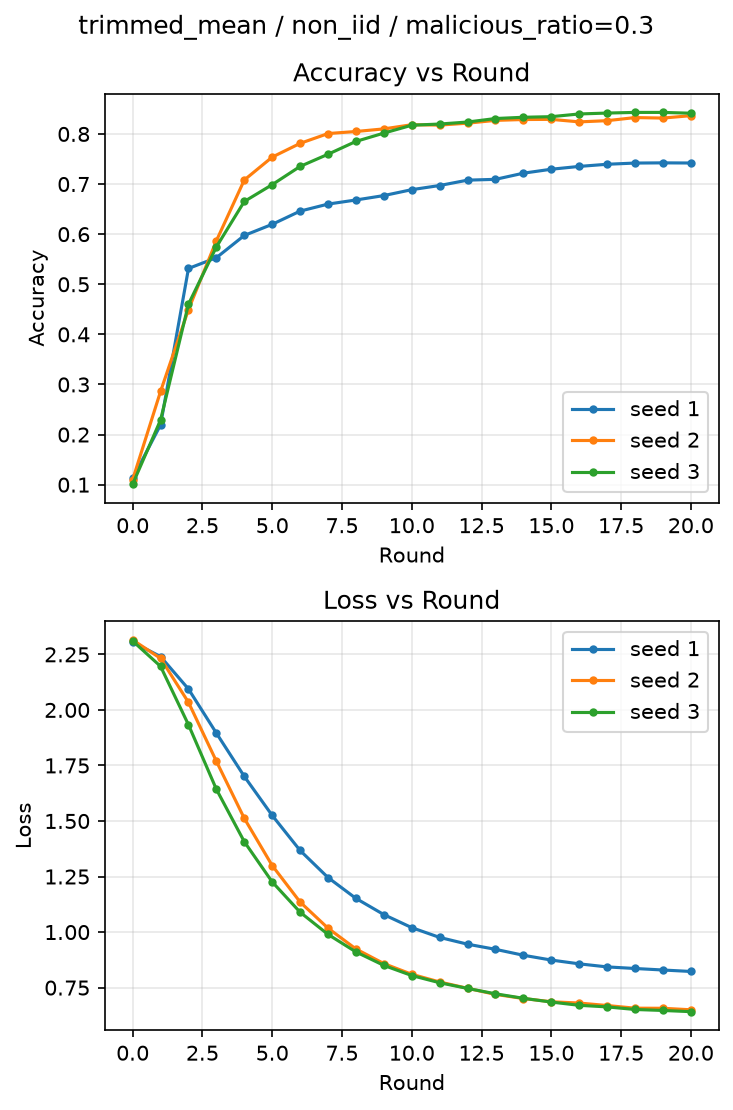
\includegraphics[width=\columnwidth]{seed_curves_trimmed_mean_non_iid_ratio0.3.png}
    \caption{Seed ごとの Round-Accuracy および Round-Loss の推移（Non-IID，悪性クライアント比率 0.3）}
    \label{fig:seed_curves_trimmed_mean_non_iid_ratio0.3}
\end{figure}
% =========================================================
\subsubsection{結果}
% =========================================================

表\ref{tab:trimmed_mean_non_iid_ratio0.3}に，各ラウンドにおける
Accuracy および Loss を示す．

学習開始時（Round 0）の Accuracy は約 0.1010--0.1125 であったが，Round 1 では約 0.2194--0.2862 まで上昇した． その後も学習ラウンドの進行に伴って Accuracy は継続的に向上し，Round 20 ではすべての Seed において約 0.7420--0.8414 に達した． Round 20 時点の Loss は約 0.6418--0.8227 であった． 悪性クライアント比率 0.0 の場合（最終 Accuracy 平均 約 0.9301）と比較すると，本条件では約 0.1234 ポイント低い水準にとどまっており，悪性クライアント比率 0.3 における攻撃の影響が最終的な Accuracy にも現れていることが分かる．

\clearpage
% =========================================================
\subsection{Trimmed Mean：Non-IID・悪性クライアント比率別の比較（Seed平均）}
% =========================================================

\subsubsection{実験条件}

\begin{itemize}
    \item \textbf{Aggregation method:} Trimmed Mean
    \item \textbf{Data split:} Non-IID
    \item \textbf{Malicious ratio:} 0.0, 0.1, 0.2, 0.3
    \item \textbf{Attack:} Adaptive attack
    \item \textbf{Number of rounds:} 20
    \item \textbf{Seeds:} 1, 2, 3（平均 $\pm$ 標準偏差）
\end{itemize}

6.1--6.4 節で示したとおり，本条件では malicious ratio 0.3 において
Seed 間で最終 Accuracy が約 0.74--0.84 と大きくばらつき，
他の malicious ratio（Seed 間の差はいずれも 0.01 未満）とは
性質が異なる．そこで 1.5--5.5 節までの Seed 1 単独比較とは異なり，
本節では malicious ratio ごとに Seed 1, 2, 3 の平均値と
標準偏差を算出し，平均線と標準偏差の帯（塗り）を重ねて比較する．
図の作成には \verb|result/plot_seed_mean_by_ratio.py| を
\verb|--aggregation trimmed_mean --split non_iid| オプションで用い，
\verb|result/results.csv| から Trimmed Mean・Non-IID の条件に一致する
run を malicious ratio ごとに抽出し，ラウンドごとの平均・標準偏差を
計算して描画した．

% =========================================================
% 実験結果図
% =========================================================

\begin{figure}[H]
    \centering
    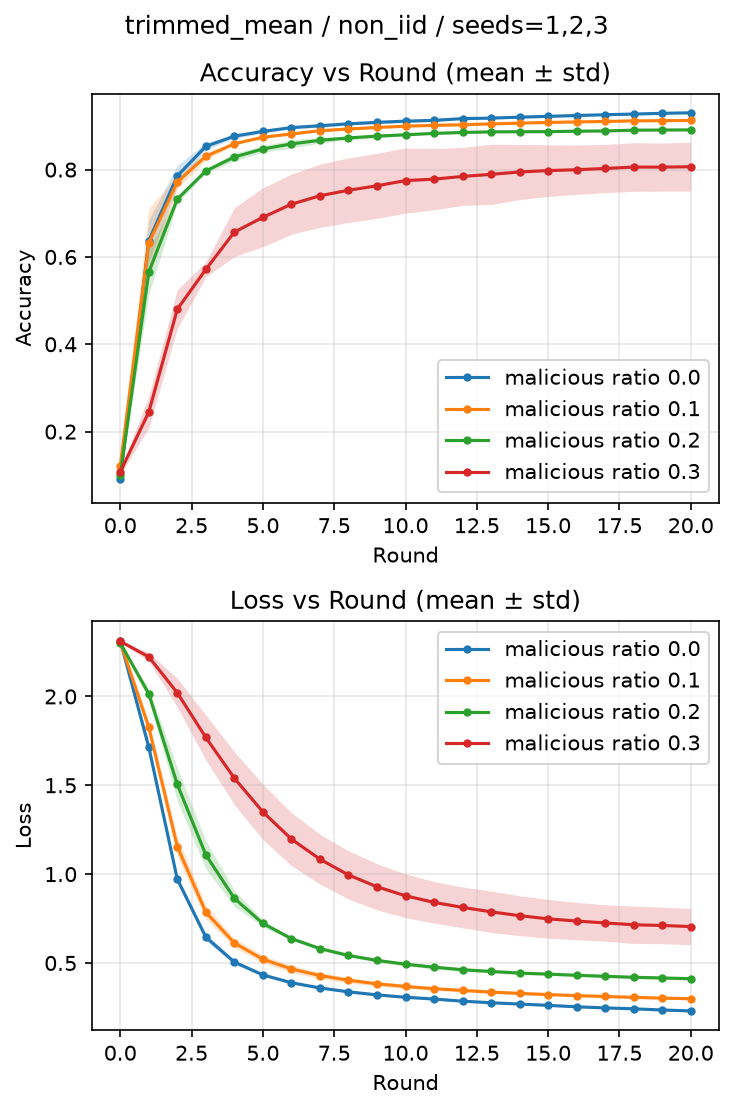
\includegraphics[width=\columnwidth]{trimmed_mean_noniid_seedmean_by_ratio.png}
    \caption{Trimmed Mean・Non-IID における malicious ratio 別の
    Round-Accuracy および Round-Loss の推移（Seed 1, 2, 3 の平均 $\pm$
    標準偏差）}
    \label{fig:trimmed_mean_noniid_seedmean_by_ratio}
\end{figure}

% =========================================================
\subsubsection{結果}
% =========================================================

図\ref{fig:trimmed_mean_noniid_seedmean_by_ratio}に，malicious ratio
0.0, 0.1, 0.2, 0.3 における Round-Accuracy および Round-Loss の
平均 $\pm$ 標準偏差の推移を示す．

Round 20 時点の平均 Accuracy（標準偏差）は，malicious ratio 0.0 で
0.9301（0.0009），ratio 0.1 で 0.9125（0.0012），ratio 0.2 で
0.8910（0.0018）であり，Seed 間のばらつきは malicious ratio に
よらずごく小さく，図上でも帯はほとんど視認できない．
一方，malicious ratio 0.3 では平均 Accuracy が 0.8066 まで低下する
のに加え，標準偏差が 0.0560 と他の malicious ratio の 30--60 倍に
達しており，図上でも Round 3 付近から Round 20 にかけて明確に
太い帯として現れている．Loss についても同様に，ratio 0.0--0.2 の
標準偏差が 0.004--0.008 にとどまるのに対し，ratio 0.3 では 0.1021
まで拡大しており，平均値の低下だけでなく Seed 間の再現性自体が
低下していることが定量的に確認できる．

以上より，Trimmed Mean は Non-IID 環境において，malicious ratio が
0.2 以下では安定した学習が再現される一方，malicious ratio 0.3 では
最終的な学習性能が Seed（乱数シード）に大きく左右される不安定な
挙動を示すことが明らかになった．

\clearpage
% =========================================================
\section{Krum（IID環境）における悪性クライアント比率別の評価}
% =========================================================

% =========================================================
\subsection{Krum：IID・悪性クライアント比率 0.0}
% =========================================================

\subsubsection{実験条件}

\begin{itemize}
    \item \textbf{Aggregation method:} Krum
    \item \textbf{Data split:} IID
    \item \textbf{Malicious ratio:} 0.0
    \item \textbf{Attack:} Adaptive attack
    \item \textbf{Number of rounds:} 20
    \item \textbf{Seeds:} 1, 2, 3
\end{itemize}

% =========================================================
% 実験結果表
% =========================================================

\begin{table}[H]
\centering

\caption{Krum（IID，悪性クライアント比率 0.0）における
Accuracy および Loss}

\label{tab:krum_iid_ratio0.0}

\footnotesize
\setlength{\tabcolsep}{2.5pt}
\renewcommand{\arraystretch}{0.90}

\resizebox{\columnwidth}{!}{%
\begin{tabular}{c cc cc cc}

\toprule

& \multicolumn{2}{c}{Seed 1}
& \multicolumn{2}{c}{Seed 2}
& \multicolumn{2}{c}{Seed 3} \\

\cmidrule(lr){2-3}
\cmidrule(lr){4-5}
\cmidrule(lr){6-7}

Round
& Acc. & Loss
& Acc. & Loss
& Acc. & Loss \\

\midrule

0 & 0.0669 & 2.3094 & 0.0459 & 2.3268 & 0.1200 & 2.3116 \\
1 & 0.6654 & 1.3536 & 0.6963 & 1.3633 & 0.6132 & 1.4078 \\
2 & 0.8040 & 0.7156 & 0.7910 & 0.7799 & 0.8060 & 0.7297 \\
3 & 0.8379 & 0.5651 & 0.8490 & 0.5839 & 0.8493 & 0.5580 \\
4 & 0.8481 & 0.4933 & 0.8566 & 0.5144 & 0.8694 & 0.4576 \\
5 & 0.8481 & 0.4787 & 0.8435 & 0.5141 & 0.8710 & 0.4432 \\
6 & 0.8676 & 0.4287 & 0.8858 & 0.4116 & 0.8940 & 0.3855 \\
7 & 0.8653 & 0.4494 & 0.8826 & 0.3994 & 0.8966 & 0.3601 \\
8 & 0.8750 & 0.3909 & 0.8822 & 0.3993 & 0.8845 & 0.3814 \\
9 & 0.8863 & 0.3692 & 0.8844 & 0.3868 & 0.8932 & 0.3532 \\
10 & 0.8684 & 0.4149 & 0.8982 & 0.3523 & 0.9020 & 0.3328 \\
11 & 0.8797 & 0.3838 & 0.9050 & 0.3223 & 0.8910 & 0.3585 \\
12 & 0.9001 & 0.3273 & 0.8958 & 0.3538 & 0.9000 & 0.3401 \\
13 & 0.8974 & 0.3456 & 0.8875 & 0.3540 & 0.8780 & 0.3990 \\
14 & 0.9032 & 0.3244 & 0.9042 & 0.3261 & 0.9027 & 0.3198 \\
15 & 0.8890 & 0.3556 & 0.9097 & 0.2996 & 0.8865 & 0.3622 \\
16 & 0.9030 & 0.3299 & 0.9096 & 0.2970 & 0.8877 & 0.3656 \\
17 & 0.8999 & 0.3372 & 0.9084 & 0.3039 & 0.9128 & 0.2863 \\
18 & 0.9061 & 0.3036 & 0.9190 & 0.2707 & 0.9142 & 0.2893 \\
19 & 0.9085 & 0.3037 & 0.9138 & 0.2958 & 0.9157 & 0.2732 \\
20 & 0.8947 & 0.3485 & 0.9007 & 0.3098 & 0.9130 & 0.3010 \\

\bottomrule

\end{tabular}%
}

\end{table}
\begin{figure}[H]
    \centering
    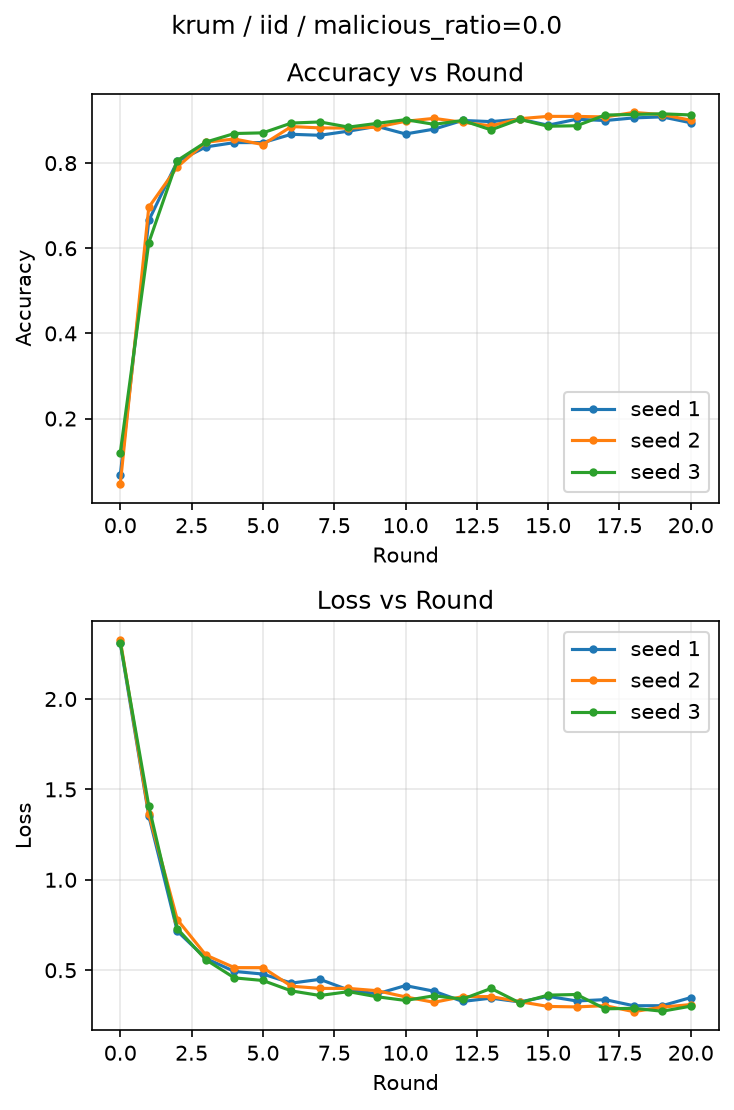
\includegraphics[width=\columnwidth]{seed_curves_krum_iid_ratio0.0.png}
    \caption{Seed ごとの Round-Accuracy および Round-Loss の推移（IID，悪性クライアント比率 0.0）}
    \label{fig:seed_curves_krum_iid_ratio0.0}
\end{figure}
% =========================================================
\subsubsection{結果}
% =========================================================

表\ref{tab:krum_iid_ratio0.0}に，各ラウンドにおける
Accuracy および Loss を示す．

学習開始時（Round 0）の Accuracy は約 0.0459--0.1200 であったが，Round 1 では約 0.6132--0.6963 まで上昇した． その後も学習ラウンドの進行に伴って Accuracy は継続的に向上し，Round 20 ではすべての Seed において約 0.8947--0.9130 に達した． Round 20 時点の Loss は約 0.3010--0.3485 であった．

\clearpage
% =========================================================
\subsection{Krum：IID・悪性クライアント比率 0.1}
% =========================================================

\subsubsection{実験条件}

\begin{itemize}
    \item \textbf{Aggregation method:} Krum
    \item \textbf{Data split:} IID
    \item \textbf{Malicious ratio:} 0.1
    \item \textbf{Attack:} Adaptive attack
    \item \textbf{Number of rounds:} 20
    \item \textbf{Seeds:} 1, 2, 3
\end{itemize}

% =========================================================
% 実験結果表
% =========================================================

\begin{table}[H]
\centering

\caption{Krum（IID，悪性クライアント比率 0.1）における
Accuracy および Loss}

\label{tab:krum_iid_ratio0.1}

\footnotesize
\setlength{\tabcolsep}{2.5pt}
\renewcommand{\arraystretch}{0.90}

\resizebox{\columnwidth}{!}{%
\begin{tabular}{c cc cc cc}

\toprule

& \multicolumn{2}{c}{Seed 1}
& \multicolumn{2}{c}{Seed 2}
& \multicolumn{2}{c}{Seed 3} \\

\cmidrule(lr){2-3}
\cmidrule(lr){4-5}
\cmidrule(lr){6-7}

Round
& Acc. & Loss
& Acc. & Loss
& Acc. & Loss \\

\midrule

0 & 0.1103 & 2.2945 & 0.0624 & 2.3102 & 0.1037 & 2.3111 \\
1 & 0.5816 & 1.9091 & 0.5125 & 2.0397 & 0.5288 & 2.0496 \\
2 & 0.7897 & 1.2345 & 0.7858 & 1.3710 & 0.7854 & 1.3508 \\
3 & 0.8375 & 0.8879 & 0.8418 & 0.9425 & 0.8301 & 0.9558 \\
4 & 0.8533 & 0.7452 & 0.8583 & 0.7722 & 0.8510 & 0.7919 \\
5 & 0.8611 & 0.6915 & 0.8660 & 0.7030 & 0.8649 & 0.7118 \\
6 & 0.8702 & 0.6401 & 0.8705 & 0.6664 & 0.8700 & 0.6726 \\
7 & 0.8729 & 0.6199 & 0.8721 & 0.6439 & 0.8756 & 0.6411 \\
8 & 0.8734 & 0.5998 & 0.8723 & 0.6293 & 0.8779 & 0.6191 \\
9 & 0.8743 & 0.5868 & 0.8729 & 0.6211 & 0.8786 & 0.6025 \\
10 & 0.8756 & 0.5828 & 0.8704 & 0.6225 & 0.8813 & 0.5932 \\
11 & 0.8749 & 0.5754 & 0.8716 & 0.6146 & 0.8836 & 0.5762 \\
12 & 0.8775 & 0.5668 & 0.8707 & 0.6104 & 0.8845 & 0.5828 \\
13 & 0.8743 & 0.5683 & 0.8680 & 0.6139 & 0.8841 & 0.5761 \\
14 & 0.8752 & 0.5692 & 0.8693 & 0.6096 & 0.8853 & 0.5699 \\
15 & 0.8764 & 0.5635 & 0.8665 & 0.6072 & 0.8858 & 0.5584 \\
16 & 0.8763 & 0.5636 & 0.8637 & 0.6055 & 0.8816 & 0.5777 \\
17 & 0.8741 & 0.5647 & 0.8590 & 0.6178 & 0.8825 & 0.5758 \\
18 & 0.8746 & 0.5622 & 0.8548 & 0.6087 & 0.8827 & 0.5725 \\
19 & 0.8756 & 0.5694 & 0.8570 & 0.5980 & 0.8778 & 0.5838 \\
20 & 0.8760 & 0.5765 & 0.8519 & 0.6155 & 0.8780 & 0.5728 \\

\bottomrule

\end{tabular}%
}

\end{table}
\begin{figure}[H]
    \centering
    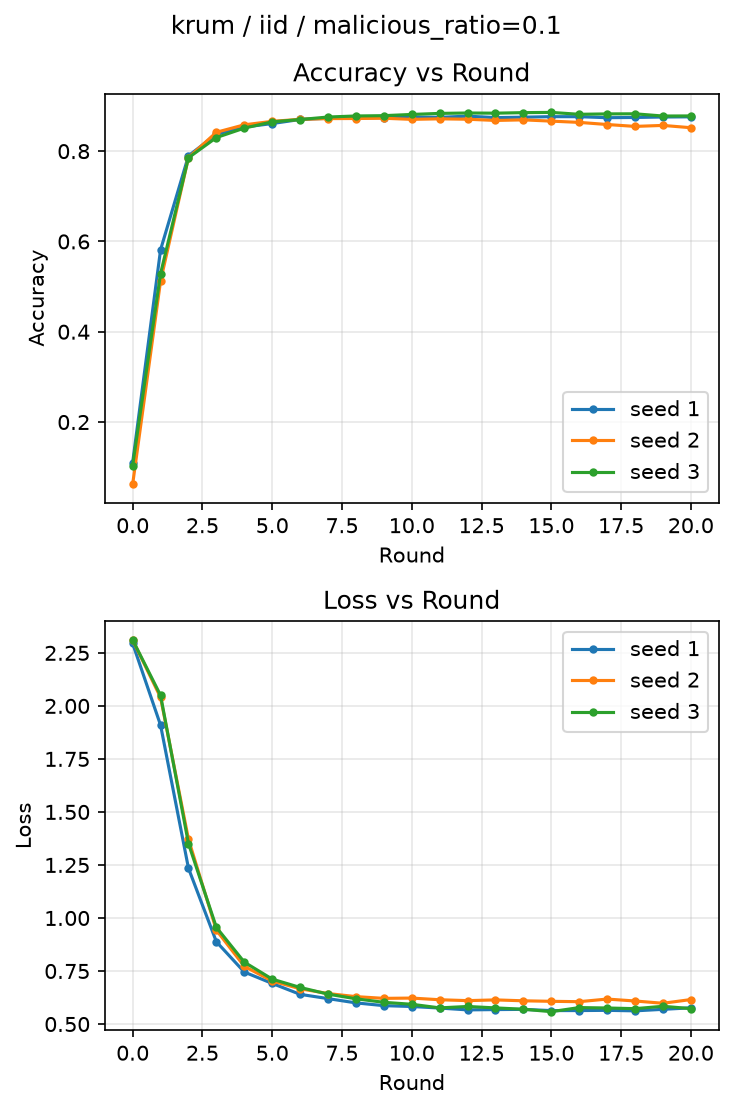
\includegraphics[width=\columnwidth]{seed_curves_krum_iid_ratio0.1.png}
    \caption{Seed ごとの Round-Accuracy および Round-Loss の推移（IID，悪性クライアント比率 0.1）}
    \label{fig:seed_curves_krum_iid_ratio0.1}
\end{figure}
% =========================================================
\subsubsection{結果}
% =========================================================

表\ref{tab:krum_iid_ratio0.1}に，各ラウンドにおける
Accuracy および Loss を示す．

学習開始時（Round 0）の Accuracy は約 0.0624--0.1103 であったが，Round 1 では約 0.5125--0.5816 まで上昇した． その後 Round 9 付近にかけて Accuracy は最大約 0.8729 まで上昇したが，その後は低下に転じ，Round 20 時点では約 0.8519--0.8780 まで悪化した． 標準的な Krum（本実験では multi\_k=1）は，複数クライアントの更新を平均せずスコアが最小となる1クライアントの更新をそのまま次ラウンドの大域モデルとして採用するため，平均化によるノイズ低減効果を持たない．Adaptive attack は過去のラウンドの大域モデルを観測しながら悪性更新を作成するため，学習が進むにつれて「多数派に近い」と Krum に誤認識されやすい悪性更新を生成できるようになり，一定ラウンド以降に悪性クライアントの更新が選択される頻度が高まってAccuracy の低下を招いたと考えられる． Round 20 時点の Loss は約 0.5728--0.6155 であった． 悪性クライアント比率 0.0 の場合（最終 Accuracy 平均 約 0.9028）と比較すると，本条件では約 0.0342 ポイント低い水準にとどまっており，悪性クライアント比率 0.1 における攻撃の影響が最終的な Accuracy にも現れていることが分かる．

\clearpage
% =========================================================
\subsection{Krum：IID・悪性クライアント比率 0.2}
% =========================================================

\subsubsection{実験条件}

\begin{itemize}
    \item \textbf{Aggregation method:} Krum
    \item \textbf{Data split:} IID
    \item \textbf{Malicious ratio:} 0.2
    \item \textbf{Attack:} Adaptive attack
    \item \textbf{Number of rounds:} 20
    \item \textbf{Seeds:} 1, 2, 3
\end{itemize}

% =========================================================
% 実験結果表
% =========================================================

\begin{table}[H]
\centering

\caption{Krum（IID，悪性クライアント比率 0.2）における
Accuracy および Loss}

\label{tab:krum_iid_ratio0.2}

\footnotesize
\setlength{\tabcolsep}{2.5pt}
\renewcommand{\arraystretch}{0.90}

\resizebox{\columnwidth}{!}{%
\begin{tabular}{c cc cc cc}

\toprule

& \multicolumn{2}{c}{Seed 1}
& \multicolumn{2}{c}{Seed 2}
& \multicolumn{2}{c}{Seed 3} \\

\cmidrule(lr){2-3}
\cmidrule(lr){4-5}
\cmidrule(lr){6-7}

Round
& Acc. & Loss
& Acc. & Loss
& Acc. & Loss \\

\midrule

0 & 0.1141 & 2.2999 & 0.0896 & 2.3316 & 0.1132 & 2.3115 \\
1 & 0.3042 & 2.1702 & 0.2339 & 2.2387 & 0.3308 & 2.1603 \\
2 & 0.7097 & 1.6720 & 0.6163 & 1.7270 & 0.6677 & 1.6026 \\
3 & 0.8094 & 1.1945 & 0.7792 & 1.1893 & 0.7927 & 1.1403 \\
4 & 0.8426 & 0.9396 & 0.8114 & 0.9519 & 0.8257 & 0.9184 \\
5 & 0.8502 & 0.8332 & 0.8242 & 0.8458 & 0.8393 & 0.8244 \\
6 & 0.8553 & 0.7717 & 0.8299 & 0.7913 & 0.8443 & 0.7836 \\
7 & 0.8524 & 0.7544 & 0.8317 & 0.7641 & 0.8480 & 0.7590 \\
8 & 0.8506 & 0.7324 & 0.8348 & 0.7477 & 0.8477 & 0.7438 \\
9 & 0.8487 & 0.7243 & 0.8338 & 0.7409 & 0.8457 & 0.7395 \\
10 & 0.8410 & 0.7265 & 0.8401 & 0.7197 & 0.8443 & 0.7342 \\
11 & 0.8369 & 0.7186 & 0.8431 & 0.7159 & 0.8438 & 0.7308 \\
12 & 0.8264 & 0.7286 & 0.8350 & 0.7392 & 0.8520 & 0.7111 \\
13 & 0.8255 & 0.7287 & 0.8306 & 0.7329 & 0.8471 & 0.7275 \\
14 & 0.8268 & 0.7258 & 0.8229 & 0.7468 & 0.8505 & 0.7039 \\
15 & 0.8237 & 0.7389 & 0.8103 & 0.7518 & 0.8435 & 0.7368 \\
16 & 0.8159 & 0.7401 & 0.8001 & 0.7571 & 0.8441 & 0.7328 \\
17 & 0.7945 & 0.7840 & 0.7936 & 0.7520 & 0.8399 & 0.7435 \\
18 & 0.8027 & 0.7603 & 0.7629 & 0.7958 & 0.8388 & 0.7424 \\
19 & 0.7648 & 0.8161 & 0.7541 & 0.8009 & 0.8357 & 0.7447 \\
20 & 0.7397 & 0.8616 & 0.7260 & 0.8398 & 0.8165 & 0.7971 \\

\bottomrule

\end{tabular}%
}

\end{table}
\begin{figure}[H]
    \centering
    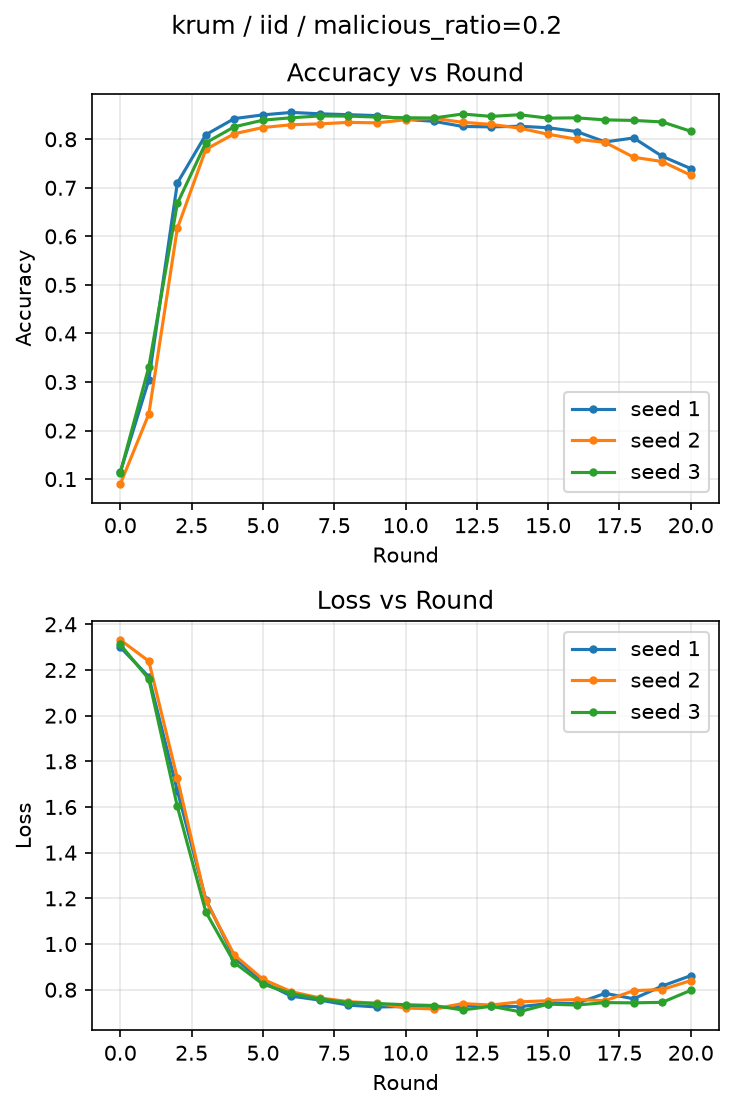
\includegraphics[width=\columnwidth]{seed_curves_krum_iid_ratio0.2.png}
    \caption{Seed ごとの Round-Accuracy および Round-Loss の推移（IID，悪性クライアント比率 0.2）}
    \label{fig:seed_curves_krum_iid_ratio0.2}
\end{figure}
% =========================================================
\subsubsection{結果}
% =========================================================

表\ref{tab:krum_iid_ratio0.2}に，各ラウンドにおける
Accuracy および Loss を示す．

学習開始時（Round 0）の Accuracy は約 0.0896--0.1141 であったが，Round 1 では約 0.2339--0.3308 まで上昇した． その後 Round 6--12 付近にかけて Accuracy は最大約 0.8553 まで上昇したが，その後は低下に転じ，Round 20 時点では約 0.7260--0.8165 まで悪化した． 標準的な Krum（本実験では multi\_k=1）は，複数クライアントの更新を平均せずスコアが最小となる1クライアントの更新をそのまま次ラウンドの大域モデルとして採用するため，平均化によるノイズ低減効果を持たない．Adaptive attack は過去のラウンドの大域モデルを観測しながら悪性更新を作成するため，学習が進むにつれて「多数派に近い」と Krum に誤認識されやすい悪性更新を生成できるようになり，一定ラウンド以降に悪性クライアントの更新が選択される頻度が高まってAccuracy の低下を招いたと考えられる． Round 20 時点の Loss は約 0.7971--0.8616 であった． 悪性クライアント比率 0.0 の場合（最終 Accuracy 平均 約 0.9028）と比較すると，本条件では約 0.1421 ポイント低い水準にとどまっており，悪性クライアント比率 0.2 における攻撃の影響が最終的な Accuracy にも現れていることが分かる．

\clearpage
% =========================================================
\subsection{Krum：IID・悪性クライアント比率 0.3}
% =========================================================

\subsubsection{実験条件}

\begin{itemize}
    \item \textbf{Aggregation method:} Krum
    \item \textbf{Data split:} IID
    \item \textbf{Malicious ratio:} 0.3
    \item \textbf{Attack:} Adaptive attack
    \item \textbf{Number of rounds:} 20
    \item \textbf{Seeds:} 1, 2, 3
\end{itemize}

% =========================================================
% 実験結果表
% =========================================================

\begin{table}[H]
\centering

\caption{Krum（IID，悪性クライアント比率 0.3）における
Accuracy および Loss}

\label{tab:krum_iid_ratio0.3}

\footnotesize
\setlength{\tabcolsep}{2.5pt}
\renewcommand{\arraystretch}{0.90}

\resizebox{\columnwidth}{!}{%
\begin{tabular}{c cc cc cc}

\toprule

& \multicolumn{2}{c}{Seed 1}
& \multicolumn{2}{c}{Seed 2}
& \multicolumn{2}{c}{Seed 3} \\

\cmidrule(lr){2-3}
\cmidrule(lr){4-5}
\cmidrule(lr){6-7}

Round
& Acc. & Loss
& Acc. & Loss
& Acc. & Loss \\

\midrule

0 & 0.0862 & 2.3106 & 0.1343 & 2.3053 & 0.0939 & 2.3091 \\
1 & 0.0936 & 2.3345 & 0.0699 & 2.3208 & 0.1075 & 2.3239 \\
2 & 0.1545 & 2.2828 & 0.1665 & 2.2652 & 0.2115 & 2.2329 \\
3 & 0.3163 & 2.0070 & 0.4084 & 2.0168 & -- & -- \\
4 & 0.5174 & 1.6533 & 0.6281 & 1.6679 & -- & -- \\
5 & 0.6450 & 1.3326 & 0.7083 & 1.3836 & -- & -- \\
6 & 0.6873 & 1.1758 & 0.7379 & 1.2313 & -- & -- \\
7 & 0.6971 & 1.0978 & 0.7597 & 1.1502 & -- & -- \\
8 & 0.6584 & 1.0996 & 0.7555 & 1.0944 & -- & -- \\
9 & 0.6410 & 1.0842 & 0.7557 & 1.0735 & -- & -- \\
10 & 0.5967 & 1.1223 & 0.7502 & 1.0497 & -- & -- \\
11 & 0.5637 & 1.1609 & 0.7220 & 1.0633 & -- & -- \\
12 & 0.5181 & 1.2326 & 0.7012 & 1.0777 & -- & -- \\
13 & 0.5036 & 1.2529 & 0.6622 & 1.1111 & -- & -- \\
14 & 0.4591 & 1.3394 & 0.6250 & 1.1536 & -- & -- \\
15 & 0.4292 & 1.4095 & 0.5374 & 1.2666 & -- & -- \\
16 & 0.4489 & 1.4029 & 0.5130 & 1.2870 & -- & -- \\
17 & 0.4200 & 1.4841 & 0.4546 & 1.3930 & -- & -- \\
18 & 0.4311 & 1.4943 & 0.4349 & 1.4194 & -- & -- \\
19 & 0.4154 & 1.5957 & 0.4067 & 1.5500 & -- & -- \\
20 & 0.4585 & 1.5063 & 0.4001 & 1.5308 & -- & -- \\

\bottomrule

\end{tabular}%
}

\end{table}
\begin{figure}[H]
    \centering
    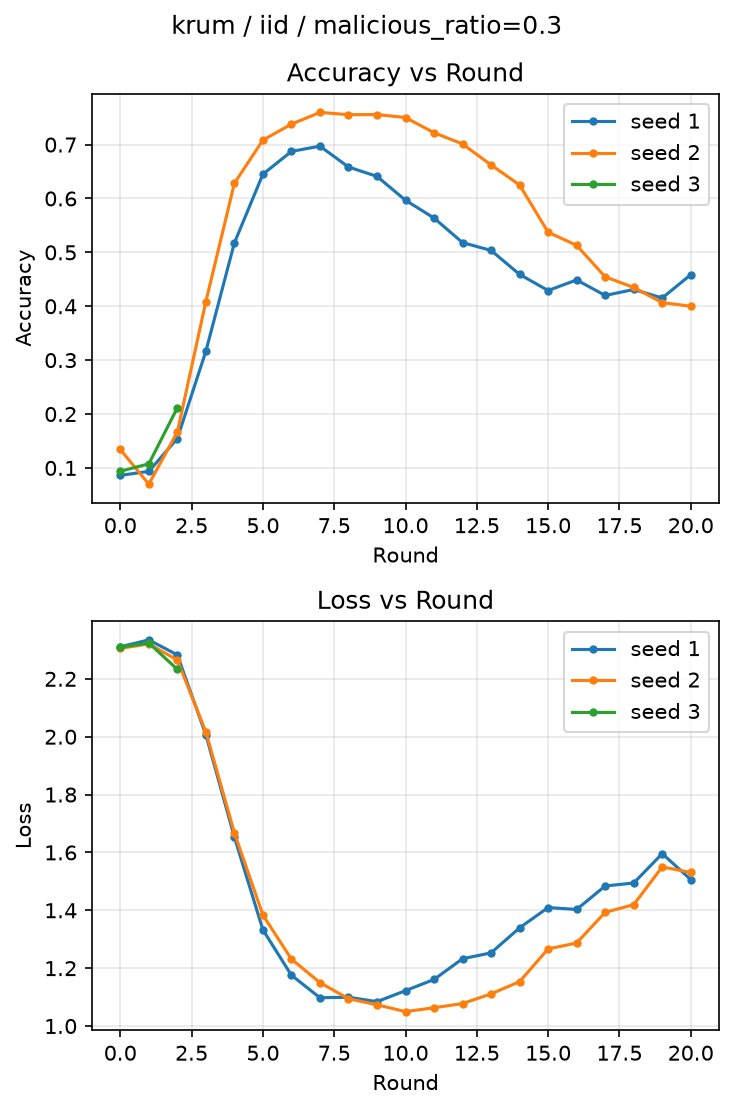
\includegraphics[width=\columnwidth]{seed_curves_krum_iid_ratio0.3.png}
    \caption{Seed ごとの Round-Accuracy および Round-Loss の推移（IID，悪性クライアント比率 0.3）}
    \label{fig:seed_curves_krum_iid_ratio0.3}
\end{figure}
% =========================================================
\subsubsection{結果}
% =========================================================

表\ref{tab:krum_iid_ratio0.3}に，各ラウンドにおける
Accuracy および Loss を示す．

学習開始時（Round 0）の Accuracy は約 0.0862--0.1343 であったが，Round 1 では約 0.0699--0.1075 まで上昇した． その後 Round 7 付近にかけて Accuracy は最大約 0.7597 まで上昇したが，その後は低下に転じ，Round 20 時点では約 0.4001--0.4585 まで悪化した． 標準的な Krum（本実験では multi\_k=1）は，複数クライアントの更新を平均せずスコアが最小となる1クライアントの更新をそのまま次ラウンドの大域モデルとして採用するため，平均化によるノイズ低減効果を持たない．Adaptive attack は過去のラウンドの大域モデルを観測しながら悪性更新を作成するため，学習が進むにつれて「多数派に近い」と Krum に誤認識されやすい悪性更新を生成できるようになり，一定ラウンド以降に悪性クライアントの更新が選択される頻度が高まってAccuracy の低下を招いたと考えられる． Round 20 時点の Loss は約 1.5063--1.5308 であった． 悪性クライアント比率 0.0 の場合（最終 Accuracy 平均 約 0.9028）と比較すると，本条件では約 0.4735 ポイント低い水準にとどまっており，悪性クライアント比率 0.3 における攻撃の影響が最終的な Accuracy にも現れていることが分かる．

なお，Seed 3（Round 2 まで） は Round 20 到達前にログが途切れており，実験が途中で終了したものと考えられる（原因不明のため，欠損箇所は表中で「--」と表記した）．

\clearpage
% =========================================================
\subsection{Krum：IID・悪性クライアント比率別の比較（Seed平均）}
% =========================================================

\subsubsection{実験条件}

\begin{itemize}
    \item \textbf{Aggregation method:} Krum
    \item \textbf{Data split:} IID
    \item \textbf{Malicious ratio:} 0.0, 0.1, 0.2, 0.3
    \item \textbf{Attack:} Adaptive attack
    \item \textbf{Number of rounds:} 20
    \item \textbf{Seeds:} 1, 2, 3（平均 $\pm$ 標準偏差）
\end{itemize}

Krum は複数クライアントの更新を平均せず，スコアが最小となる
1クライアントの更新のみを採用するため，Trimmed Mean や Median と
異なり malicious ratio 0.0（悪性クライアントが存在しない場合）でも
Round ごとの Accuracy・Loss の変動が大きい．
そこで本節でも 6.5 節と同様に，malicious ratio ごとに
Seed 1, 2, 3（一部 Round でログが途切れた Seed を除く，利用可能な
Seed のみ）の平均値と標準偏差を算出し，平均線と標準偏差の帯を
重ねて比較する．
図の作成には \verb|result/plot_seed_mean_by_ratio.py| を
\verb|--aggregation krum --split iid| オプションで用い，
\verb|result/results.csv| から Krum・IID の条件に一致する run を
malicious ratio ごとに抽出し，ラウンドごとの平均・標準偏差を
計算して描画した．

% =========================================================
% 実験結果図
% =========================================================

\begin{figure}[H]
    \centering
    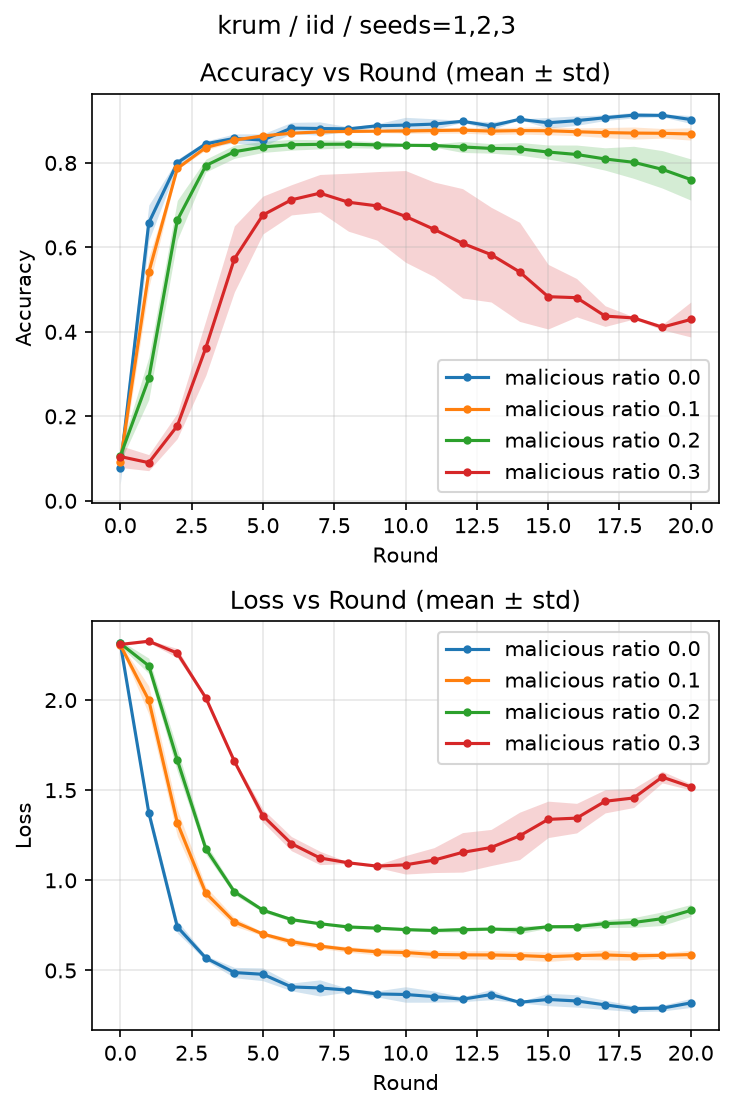
\includegraphics[width=\columnwidth]{krum_iid_seedmean_by_ratio.png}
    \caption{Krum・IID における malicious ratio 別の
    Round-Accuracy および Round-Loss の推移（Seed 平均 $\pm$
    標準偏差）}
    \label{fig:krum_iid_seedmean_by_ratio}
\end{figure}

% =========================================================
\subsubsection{結果}
% =========================================================

図\ref{fig:krum_iid_seedmean_by_ratio}に，malicious ratio
0.0, 0.1, 0.2, 0.3 における Round-Accuracy および Round-Loss の
平均 $\pm$ 標準偏差の推移を示す．

malicious ratio 0.0 では Accuracy が Round 18 付近で平均 0.9131 の
ピークに達した後 Round 20 では 0.9028（標準偏差 0.0093）とほぼ
横ばいであるのに対し，malicious ratio 0.1 では Round 12 付近の
ピーク（平均 0.8776）から Round 20 の 0.8686（標準偏差 0.0145）へと
わずかに低下する．malicious ratio 0.2 では Round 8 付近のピーク
（平均 0.8444）から Round 20 の 0.7607（標準偏差 0.0488）へ，
malicious ratio 0.3 では Round 7 付近のピーク（平均 0.7284）から
Round 20 の 0.4293（標準偏差 0.0413，Round 20 まで残存した Seed は
2 個）へと大きく低下しており，malicious ratio が高いほど
「Accuracy が一度ピークに達した後に低下する」傾向がより早く・
より大きく現れることが分かる．また標準偏差も malicious ratio 0.0
の 0.0093 から malicious ratio 0.2 の 0.0488 へと増加しており，
攻撃が進むにつれて Seed 間の再現性も低下する．

以上より，Krum は malicious ratio の増加に伴って最終的な
Accuracy が低下するだけでなく，学習後半にかけて性能が悪化する
「後退」現象がより顕著になり，Seed 間のばらつきも拡大することが
確認された．

\clearpage
% =========================================================
\section{Krum（Non-IID環境）における悪性クライアント比率別の評価}
% =========================================================

% =========================================================
\subsection{Krum：Non-IID・悪性クライアント比率 0.0}
% =========================================================

\subsubsection{実験条件}

\begin{itemize}
    \item \textbf{Aggregation method:} Krum
    \item \textbf{Data split:} Non-IID
    \item \textbf{Malicious ratio:} 0.0
    \item \textbf{Attack:} Adaptive attack
    \item \textbf{Number of rounds:} 20
    \item \textbf{Seeds:} 1, 2, 3
\end{itemize}

% =========================================================
% 実験結果表
% =========================================================

\begin{table}[H]
\centering

\caption{Krum（Non-IID，悪性クライアント比率 0.0）における
Accuracy および Loss}

\label{tab:krum_non_iid_ratio0.0}

\footnotesize
\setlength{\tabcolsep}{2.5pt}
\renewcommand{\arraystretch}{0.90}

\resizebox{\columnwidth}{!}{%
\begin{tabular}{c cc cc cc}

\toprule

& \multicolumn{2}{c}{Seed 1}
& \multicolumn{2}{c}{Seed 2}
& \multicolumn{2}{c}{Seed 3} \\

\cmidrule(lr){2-3}
\cmidrule(lr){4-5}
\cmidrule(lr){6-7}

Round
& Acc. & Loss
& Acc. & Loss
& Acc. & Loss \\

\midrule

0 & 0.0853 & 2.3167 & 0.1254 & 2.3149 & 0.0829 & 2.3103 \\
1 & 0.2912 & 2.2931 & 0.1751 & 2.2551 & 0.0900 & 2.3988 \\
2 & 0.3089 & 2.1787 & 0.3036 & 2.2109 & -- & -- \\
3 & 0.3833 & 2.0338 & 0.3628 & 1.9829 & -- & -- \\
4 & 0.5630 & 1.8468 & 0.4208 & 1.6466 & -- & -- \\
5 & 0.5149 & 1.4442 & 0.6377 & 1.2436 & -- & -- \\
6 & 0.6824 & 1.1318 & 0.7762 & 0.8342 & -- & -- \\
7 & 0.6251 & 1.2006 & 0.7833 & 0.7288 & -- & -- \\
8 & 0.6791 & 1.1829 & 0.6778 & 0.9458 & -- & -- \\
9 & 0.6637 & 1.0085 & 0.7448 & 0.7731 & -- & -- \\
10 & 0.5873 & 1.1679 & 0.7325 & 0.7798 & -- & -- \\
11 & 0.6636 & 1.0479 & 0.7638 & 0.7147 & -- & -- \\
12 & 0.7596 & 0.7871 & 0.7403 & 0.7575 & -- & -- \\
13 & 0.7140 & 0.8338 & 0.7388 & 0.8062 & -- & -- \\
14 & 0.7747 & 0.7363 & 0.6180 & 1.2204 & -- & -- \\
15 & 0.6659 & 0.9738 & 0.8188 & 0.5781 & -- & -- \\
16 & 0.7464 & 0.8033 & 0.6732 & 1.0473 & -- & -- \\
17 & 0.6448 & 1.1147 & 0.7312 & 0.8090 & -- & -- \\
18 & 0.6763 & 0.9504 & 0.7310 & 0.8895 & -- & -- \\
19 & 0.7025 & 0.8551 & 0.7557 & 0.7709 & -- & -- \\
20 & 0.7883 & 0.7358 & 0.7407 & 0.8119 & -- & -- \\

\bottomrule

\end{tabular}%
}

\end{table}
\begin{figure}[H]
    \centering
    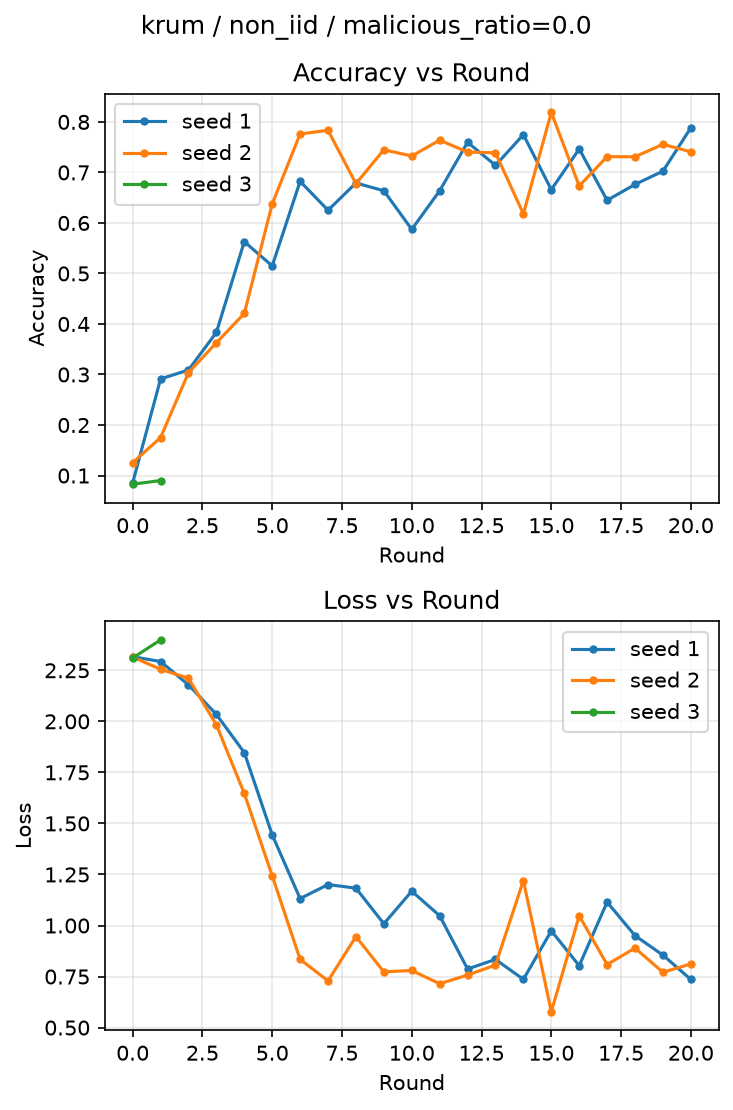
\includegraphics[width=\columnwidth]{seed_curves_krum_non_iid_ratio0.0.png}
    \caption{Seed ごとの Round-Accuracy および Round-Loss の推移（Non-IID，悪性クライアント比率 0.0）}
    \label{fig:seed_curves_krum_non_iid_ratio0.0}
\end{figure}
% =========================================================
\subsubsection{結果}
% =========================================================

表\ref{tab:krum_non_iid_ratio0.0}に，各ラウンドにおける
Accuracy および Loss を示す．

学習開始時（Round 0）の Accuracy は約 0.0829--0.1254 であったが，Round 1 では約 0.0900--0.2912 まで上昇した． その後 Round 15 付近にかけて Accuracy は最大約 0.8188 まで上昇したが，その後は低下に転じ，Round 20 時点では約 0.7407--0.7883 まで悪化した． 標準的な Krum（本実験では multi\_k=1）は，複数クライアントの更新を平均せずスコアが最小となる1クライアントの更新をそのまま次ラウンドの大域モデルとして採用するため，平均化によるノイズ低減効果を持たない．Adaptive attack は過去のラウンドの大域モデルを観測しながら悪性更新を作成するため，学習が進むにつれて「多数派に近い」と Krum に誤認識されやすい悪性更新を生成できるようになり，一定ラウンド以降に悪性クライアントの更新が選択される頻度が高まってAccuracy の低下を招いたと考えられる． Round 20 時点の Loss は約 0.7358--0.8119 であった．

なお，Seed 3（Round 1 まで） は Round 20 到達前にログが途切れており，実験が途中で終了したものと考えられる（原因不明のため，欠損箇所は表中で「--」と表記した）．

\clearpage
% =========================================================
\subsection{Krum：Non-IID・悪性クライアント比率 0.1}
% =========================================================

\subsubsection{実験条件}

\begin{itemize}
    \item \textbf{Aggregation method:} Krum
    \item \textbf{Data split:} Non-IID
    \item \textbf{Malicious ratio:} 0.1
    \item \textbf{Attack:} Adaptive attack
    \item \textbf{Number of rounds:} 20
    \item \textbf{Seeds:} 1, 2, 3
\end{itemize}

% =========================================================
% 実験結果表
% =========================================================

\begin{table}[H]
\centering

\caption{Krum（Non-IID，悪性クライアント比率 0.1）における
Accuracy および Loss}

\label{tab:krum_non_iid_ratio0.1}

\footnotesize
\setlength{\tabcolsep}{2.5pt}
\renewcommand{\arraystretch}{0.90}

\resizebox{\columnwidth}{!}{%
\begin{tabular}{c cc cc cc}

\toprule

& \multicolumn{2}{c}{Seed 1}
& \multicolumn{2}{c}{Seed 2}
& \multicolumn{2}{c}{Seed 3} \\

\cmidrule(lr){2-3}
\cmidrule(lr){4-5}
\cmidrule(lr){6-7}

Round
& Acc. & Loss
& Acc. & Loss
& Acc. & Loss \\

\midrule

0 & 0.1163 & 2.3060 & 0.0673 & 2.3211 & 0.1305 & 2.3057 \\
1 & 0.1788 & 2.2265 & 0.2946 & 2.2301 & 0.2021 & 2.2260 \\
2 & 0.5532 & 2.0375 & 0.5455 & 2.0085 & 0.4372 & 2.0526 \\
3 & 0.6748 & 1.7758 & 0.7386 & 1.6396 & 0.6856 & 1.7906 \\
4 & 0.7319 & 1.5022 & 0.8016 & 1.3264 & 0.7564 & 1.5319 \\
5 & 0.7631 & 1.2994 & 0.8265 & 1.1070 & 0.7830 & 1.3363 \\
6 & 0.7825 & 1.1370 & 0.8411 & 0.9601 & 0.7998 & 1.1637 \\
7 & 0.8004 & 1.0144 & 0.8521 & 0.8528 & 0.8131 & 1.0334 \\
8 & 0.8131 & 0.9105 & 0.8541 & 0.7950 & 0.8185 & 0.9550 \\
9 & 0.8250 & 0.8601 & 0.8570 & 0.7422 & 0.8296 & 0.8992 \\
10 & 0.8301 & 0.8247 & 0.8618 & 0.7047 & 0.8333 & 0.8477 \\
11 & 0.8364 & 0.7772 & 0.8660 & 0.6820 & 0.8256 & 0.8215 \\
12 & 0.8378 & 0.7647 & 0.8677 & 0.6567 & 0.8289 & 0.7740 \\
13 & 0.8424 & 0.7165 & 0.8658 & 0.6606 & 0.8243 & 0.7536 \\
14 & 0.8417 & 0.7045 & 0.8696 & 0.6431 & 0.8302 & 0.7319 \\
15 & 0.8469 & 0.6763 & 0.8689 & 0.6348 & 0.8324 & 0.7067 \\
16 & 0.8481 & 0.6611 & 0.8714 & 0.6162 & 0.8287 & 0.7024 \\
17 & 0.8505 & 0.6443 & 0.8688 & 0.6159 & 0.8385 & 0.6731 \\
18 & 0.8495 & 0.6423 & 0.8674 & 0.6127 & 0.8378 & 0.6623 \\
19 & 0.8445 & 0.6575 & 0.8653 & 0.6065 & 0.8347 & 0.6592 \\
20 & 0.8419 & 0.6553 & 0.8689 & 0.5816 & 0.8341 & 0.6629 \\

\bottomrule

\end{tabular}%
}

\end{table}
\begin{figure}[H]
    \centering
    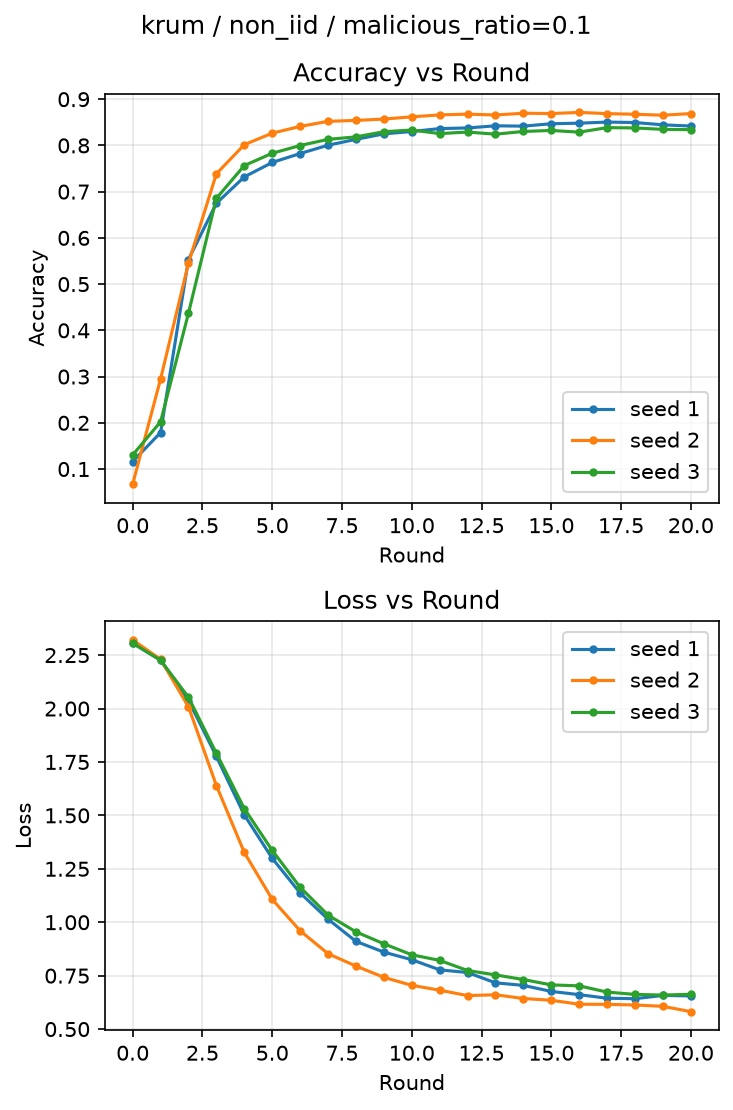
\includegraphics[width=\columnwidth]{seed_curves_krum_non_iid_ratio0.1.png}
    \caption{Seed ごとの Round-Accuracy および Round-Loss の推移（Non-IID，悪性クライアント比率 0.1）}
    \label{fig:seed_curves_krum_non_iid_ratio0.1}
\end{figure}
% =========================================================
\subsubsection{結果}
% =========================================================

表\ref{tab:krum_non_iid_ratio0.1}に，各ラウンドにおける
Accuracy および Loss を示す．

学習開始時（Round 0）の Accuracy は約 0.0673--0.1305 であったが，Round 1 では約 0.1788--0.2946 まで上昇した． その後も学習ラウンドの進行に伴って Accuracy は継続的に向上し，Round 20 ではすべての Seed において約 0.8341--0.8689 に達した． Round 20 時点の Loss は約 0.5816--0.6629 であった． 悪性クライアント比率 0.0 の場合（最終 Accuracy 平均 約 0.7645）と比較しても最終的な Accuracy に大きな差は見られず，本条件下でも学習は概ね安定していたといえる．

\clearpage
% =========================================================
\subsection{Krum：Non-IID・悪性クライアント比率 0.2}
% =========================================================

\subsubsection{実験条件}

\begin{itemize}
    \item \textbf{Aggregation method:} Krum
    \item \textbf{Data split:} Non-IID
    \item \textbf{Malicious ratio:} 0.2
    \item \textbf{Attack:} Adaptive attack
    \item \textbf{Number of rounds:} 20
    \item \textbf{Seeds:} 1, 2, 3
\end{itemize}

% =========================================================
% 実験結果表
% =========================================================

\begin{table}[H]
\centering

\caption{Krum（Non-IID，悪性クライアント比率 0.2）における
Accuracy および Loss}

\label{tab:krum_non_iid_ratio0.2}

\footnotesize
\setlength{\tabcolsep}{2.5pt}
\renewcommand{\arraystretch}{0.90}

\resizebox{\columnwidth}{!}{%
\begin{tabular}{c cc cc cc}

\toprule

& \multicolumn{2}{c}{Seed 1}
& \multicolumn{2}{c}{Seed 2}
& \multicolumn{2}{c}{Seed 3} \\

\cmidrule(lr){2-3}
\cmidrule(lr){4-5}
\cmidrule(lr){6-7}

Round
& Acc. & Loss
& Acc. & Loss
& Acc. & Loss \\

\midrule

0 & 0.1516 & 2.2851 & 0.1160 & 2.3091 & 0.1606 & 2.2927 \\
1 & 0.2509 & 2.2326 & 0.1317 & 2.3006 & 0.2149 & 2.2279 \\
2 & 0.3873 & 2.0815 & 0.1975 & 2.2646 & 0.3117 & 2.1292 \\
3 & 0.5011 & 1.8347 & 0.3867 & 2.0831 & 0.4594 & 1.9773 \\
4 & 0.5966 & 1.6404 & 0.5643 & 1.8532 & 0.5292 & 1.8219 \\
5 & 0.6720 & 1.4535 & 0.6692 & 1.6474 & 0.5794 & 1.6526 \\
6 & 0.6993 & 1.3308 & 0.7200 & 1.4513 & 0.6163 & 1.5073 \\
7 & 0.7209 & 1.2290 & 0.7402 & 1.3094 & 0.6753 & 1.3504 \\
8 & 0.7389 & 1.1443 & 0.7439 & 1.2095 & 0.7070 & 1.2258 \\
9 & 0.7437 & 1.0877 & 0.7526 & 1.1309 & 0.7311 & 1.1333 \\
10 & 0.7379 & 1.0740 & 0.7580 & 1.0692 & 0.7316 & 1.0753 \\
11 & 0.7328 & 1.0489 & 0.7639 & 1.0283 & 0.7459 & 1.0170 \\
12 & 0.6816 & 1.0894 & 0.7692 & 0.9861 & 0.7578 & 0.9596 \\
13 & 0.6475 & 1.1088 & 0.7538 & 1.0093 & 0.7629 & 0.9255 \\
14 & 0.6067 & 1.1467 & 0.7537 & 0.9883 & 0.7498 & 0.9300 \\
15 & 0.6187 & 1.0948 & 0.7598 & 0.9640 & 0.7453 & 0.9152 \\
16 & 0.6122 & 1.0880 & 0.7605 & 0.9343 & 0.7239 & 0.9381 \\
17 & 0.5765 & 1.1453 & 0.7530 & 0.9201 & 0.7368 & 0.9051 \\
18 & 0.5617 & 1.1524 & 0.7512 & 0.9205 & 0.7422 & 0.8774 \\
19 & 0.5607 & 1.1350 & 0.7230 & 0.9525 & 0.6998 & 0.9324 \\
20 & 0.5478 & 1.1518 & 0.6906 & 0.9939 & 0.6953 & 0.9166 \\

\bottomrule

\end{tabular}%
}

\end{table}
\begin{figure}[H]
    \centering
    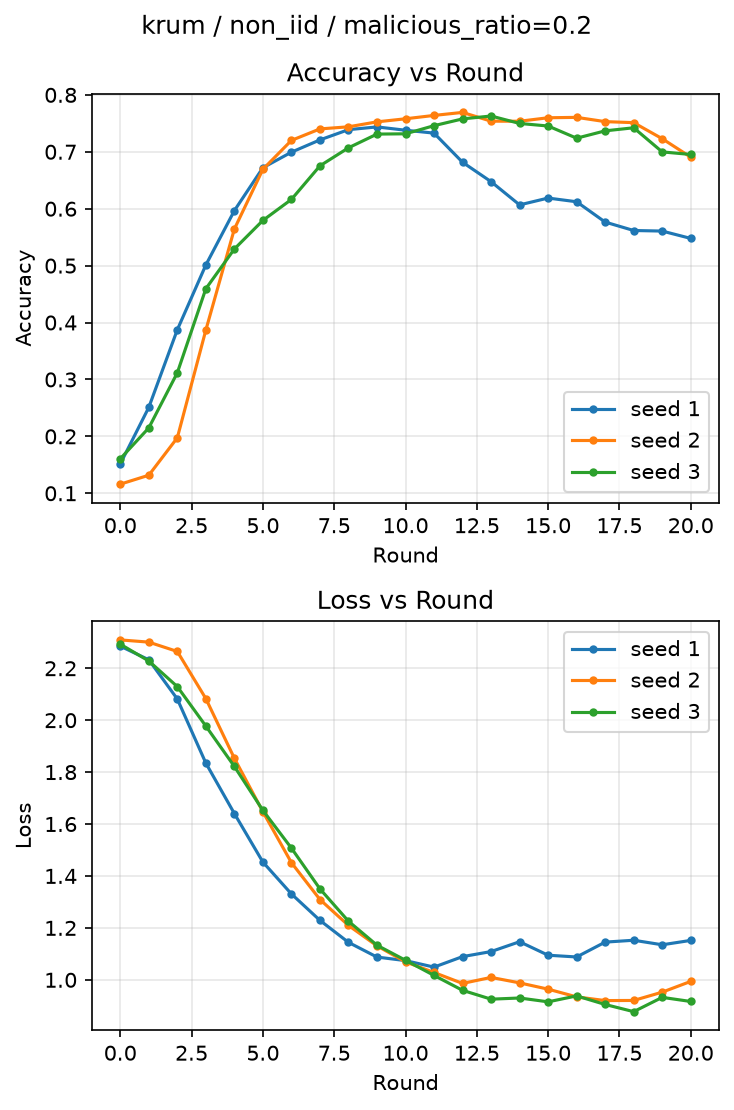
\includegraphics[width=\columnwidth]{seed_curves_krum_non_iid_ratio0.2.png}
    \caption{Seed ごとの Round-Accuracy および Round-Loss の推移（Non-IID，悪性クライアント比率 0.2）}
    \label{fig:seed_curves_krum_non_iid_ratio0.2}
\end{figure}
% =========================================================
\subsubsection{結果}
% =========================================================

表\ref{tab:krum_non_iid_ratio0.2}に，各ラウンドにおける
Accuracy および Loss を示す．

学習開始時（Round 0）の Accuracy は約 0.1160--0.1606 であったが，Round 1 では約 0.1317--0.2509 まで上昇した． その後 Round 9--13 付近にかけて Accuracy は最大約 0.7692 まで上昇したが，その後は低下に転じ，Round 20 時点では約 0.5478--0.6953 まで悪化した． 標準的な Krum（本実験では multi\_k=1）は，複数クライアントの更新を平均せずスコアが最小となる1クライアントの更新をそのまま次ラウンドの大域モデルとして採用するため，平均化によるノイズ低減効果を持たない．Adaptive attack は過去のラウンドの大域モデルを観測しながら悪性更新を作成するため，学習が進むにつれて「多数派に近い」と Krum に誤認識されやすい悪性更新を生成できるようになり，一定ラウンド以降に悪性クライアントの更新が選択される頻度が高まってAccuracy の低下を招いたと考えられる． Round 20 時点の Loss は約 0.9166--1.1518 であった． 悪性クライアント比率 0.0 の場合（最終 Accuracy 平均 約 0.7645）と比較すると，本条件では約 0.1199 ポイント低い水準にとどまっており，悪性クライアント比率 0.2 における攻撃の影響が最終的な Accuracy にも現れていることが分かる．

\clearpage
% =========================================================
\subsection{Krum：Non-IID・悪性クライアント比率 0.3}
% =========================================================

\subsubsection{実験条件}

\begin{itemize}
    \item \textbf{Aggregation method:} Krum
    \item \textbf{Data split:} Non-IID
    \item \textbf{Malicious ratio:} 0.3
    \item \textbf{Attack:} Adaptive attack
    \item \textbf{Number of rounds:} 20
    \item \textbf{Seeds:} 1, 2, 3
\end{itemize}

% =========================================================
% 実験結果表
% =========================================================

\begin{table}[H]
\centering

\caption{Krum（Non-IID，悪性クライアント比率 0.3）における
Accuracy および Loss}

\label{tab:krum_non_iid_ratio0.3}

\footnotesize
\setlength{\tabcolsep}{2.5pt}
\renewcommand{\arraystretch}{0.90}

\resizebox{\columnwidth}{!}{%
\begin{tabular}{c cc cc cc}

\toprule

& \multicolumn{2}{c}{Seed 1}
& \multicolumn{2}{c}{Seed 2}
& \multicolumn{2}{c}{Seed 3} \\

\cmidrule(lr){2-3}
\cmidrule(lr){4-5}
\cmidrule(lr){6-7}

Round
& Acc. & Loss
& Acc. & Loss
& Acc. & Loss \\

\midrule

0 & 0.0955 & 2.3223 & 0.0880 & 2.3161 & 0.0853 & 2.3133 \\
1 & 0.0577 & 2.4147 & 0.1259 & 2.3075 & 0.0401 & 2.3555 \\
2 & 0.0493 & 2.5990 & 0.1254 & 2.2936 & 0.0571 & 2.3765 \\
3 & 0.0531 & 2.9717 & 0.1431 & 2.2750 & 0.0312 & 2.4251 \\
4 & 0.0597 & 3.2527 & 0.1490 & 2.2715 & 0.0137 & 2.4819 \\
5 & 0.0497 & 3.6783 & 0.1807 & 2.3027 & 0.0203 & 2.5569 \\
6 & 0.0521 & 4.1798 & 0.1913 & 2.4265 & 0.0486 & 2.6681 \\
7 & 0.0538 & 4.5942 & 0.2106 & 2.5922 & 0.0636 & 2.8609 \\
8 & 0.0831 & 4.8242 & 0.2201 & 2.7801 & 0.0896 & 3.1301 \\
9 & 0.0888 & 4.8831 & 0.2345 & 2.8981 & 0.0916 & 3.2925 \\
10 & 0.0885 & 4.8629 & 0.2398 & 3.0228 & 0.1020 & 3.3515 \\
11 & 0.0858 & 4.8218 & 0.2499 & 2.7527 & 0.1105 & 3.4754 \\
12 & 0.0929 & 4.8677 & 0.2517 & 2.5885 & 0.1100 & 3.5737 \\
13 & 0.1175 & 4.5680 & 0.2574 & 2.5459 & 0.1064 & 3.5864 \\
14 & 0.1510 & 4.5572 & 0.2628 & 2.4127 & 0.1025 & 3.5501 \\
15 & 0.2022 & 4.2295 & 0.2684 & 2.5646 & 0.1081 & 3.4255 \\
16 & 0.2279 & 3.9989 & -- & -- & 0.1124 & 3.1675 \\
17 & 0.2507 & 3.8906 & -- & -- & 0.1148 & 3.0590 \\
18 & 0.2420 & 3.9299 & -- & -- & 0.1186 & 2.9662 \\
19 & 0.2688 & 3.8473 & -- & -- & 0.1140 & 3.2407 \\
20 & 0.2764 & 3.6817 & -- & -- & 0.1224 & 3.0000 \\

\bottomrule

\end{tabular}%
}

\end{table}
\begin{figure}[H]
    \centering
    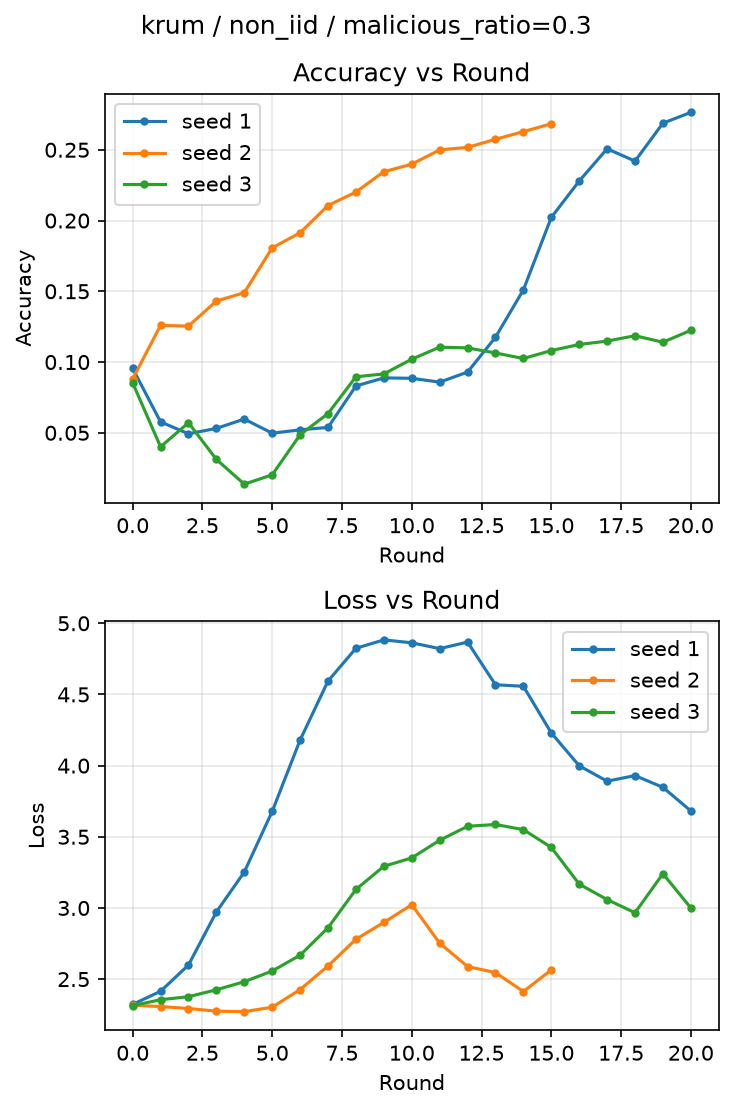
\includegraphics[width=\columnwidth]{seed_curves_krum_non_iid_ratio0.3.png}
    \caption{Seed ごとの Round-Accuracy および Round-Loss の推移（Non-IID，悪性クライアント比率 0.3）}
    \label{fig:seed_curves_krum_non_iid_ratio0.3}
\end{figure}
% =========================================================
\subsubsection{結果}
% =========================================================

表\ref{tab:krum_non_iid_ratio0.3}に，各ラウンドにおける
Accuracy および Loss を示す．

学習開始時（Round 0）の Accuracy は約 0.0853--0.0955 であったが，Round 1 では約 0.0401--0.1259 まで上昇した． その後も学習ラウンドの進行に伴って Accuracy は継続的に向上し，Round 20 ではすべての Seed において約 0.1224--0.2764 に達した． Round 20 時点の Loss は約 3.0000--3.6817 であった． 悪性クライアント比率 0.0 の場合（最終 Accuracy 平均 約 0.7645）と比較すると，本条件では約 0.5651 ポイント低い水準にとどまっており，悪性クライアント比率 0.3 における攻撃の影響が最終的な Accuracy にも現れていることが分かる．

なお，Seed 2（Round 15 まで） は Round 20 到達前にログが途切れており，実験が途中で終了したものと考えられる（原因不明のため，欠損箇所は表中で「--」と表記した）．

\clearpage
% =========================================================
\subsection{Krum：Non-IID・悪性クライアント比率別の比較（Seed平均）}
% =========================================================

\subsubsection{実験条件}

\begin{itemize}
    \item \textbf{Aggregation method:} Krum
    \item \textbf{Data split:} Non-IID
    \item \textbf{Malicious ratio:} 0.0, 0.1, 0.2, 0.3
    \item \textbf{Attack:} Adaptive attack
    \item \textbf{Number of rounds:} 20
    \item \textbf{Seeds:} 1, 2, 3（平均 $\pm$ 標準偏差）
\end{itemize}

7.5 節（Krum・IID）と同様に，malicious ratio ごとに
Seed 1, 2, 3（一部 Round でログが途切れた Seed を除く，利用可能な
Seed のみ）の平均値と標準偏差を算出し，平均線と標準偏差の帯を
重ねて比較する．
図の作成には \verb|result/plot_seed_mean_by_ratio.py| を
\verb|--aggregation krum --split non_iid| オプションで用い，
\verb|result/results.csv| から Krum・Non-IID の条件に一致する run を
malicious ratio ごとに抽出し，ラウンドごとの平均・標準偏差を
計算して描画した．

% =========================================================
% 実験結果図
% =========================================================

\begin{figure}[H]
    \centering
    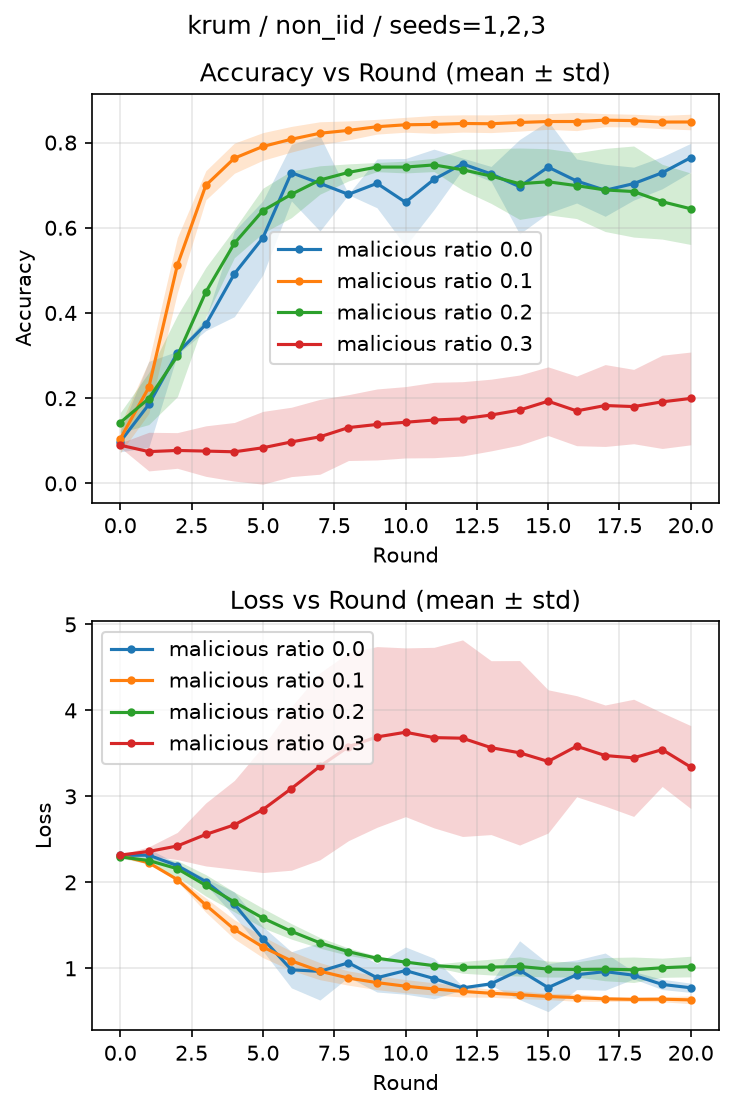
\includegraphics[width=\columnwidth]{krum_noniid_seedmean_by_ratio.png}
    \caption{Krum・Non-IID における malicious ratio 別の
    Round-Accuracy および Round-Loss の推移（Seed 平均 $\pm$
    標準偏差）}
    \label{fig:krum_noniid_seedmean_by_ratio}
\end{figure}

% =========================================================
\subsubsection{結果}
% =========================================================

図\ref{fig:krum_noniid_seedmean_by_ratio}に，malicious ratio
0.0, 0.1, 0.2, 0.3 における Round-Accuracy および Round-Loss の
平均 $\pm$ 標準偏差の推移を示す．

Round 20 時点の平均 Accuracy（標準偏差，残存 Seed 数）は，
malicious ratio 0.0 で 0.7645（0.0337，$n=2$），ratio 0.1 で
0.8483（0.0183，$n=3$），ratio 0.2 で 0.6446（0.0838，$n=3$），
ratio 0.3 で 0.1994（0.1089，$n=2$）であった．
malicious ratio 0.1 が他の malicious ratio よりも高い Accuracy を
示す逆転が見られるが，これは IID 環境の場合と異なり Non-IID 環境
では malicious ratio 0.0 の Seed 3 が Round 1 で，malicious ratio
0.2 の一部 Seed も学習後半で不安定化しており，Krum 自体が
Non-IID 環境下で本質的にノイズの大きい集約手法であることを
反映していると考えられる．一方 malicious ratio 0.3 は，
Round 9 付近から Loss が平均 3 を超えて発散気味に推移し
（Round 20 時点で平均 3.3408，標準偏差 0.4821），Accuracy も
0.2 付近から改善せず，他の malicious ratio とは明確に異なる
破綻した挙動を示した．

以上より，Krum は Non-IID 環境において IID 環境以上に
Round ごとの変動が大きく，malicious ratio 0.3 では学習がほぼ
機能しない水準まで悪化することが確認された．

\clearpage
% =========================================================
\section{Bulyan（IID環境）における悪性クライアント比率別の評価}
% =========================================================

% =========================================================
\subsection{Bulyan：IID・悪性クライアント比率 0.0}
% =========================================================

\subsubsection{実験条件}

\begin{itemize}
    \item \textbf{Aggregation method:} Bulyan
    \item \textbf{Data split:} IID
    \item \textbf{Malicious ratio:} 0.0
    \item \textbf{Attack:} Adaptive attack
    \item \textbf{Number of rounds:} 20
    \item \textbf{Seeds:} 1, 2, 3
\end{itemize}

% =========================================================
% 実験結果表
% =========================================================

\begin{table}[H]
\centering

\caption{Bulyan（IID，悪性クライアント比率 0.0）における
Accuracy および Loss}

\label{tab:bulyan_iid_ratio0.0}

\footnotesize
\setlength{\tabcolsep}{2.5pt}
\renewcommand{\arraystretch}{0.90}

\resizebox{\columnwidth}{!}{%
\begin{tabular}{c cc cc cc}

\toprule

& \multicolumn{2}{c}{Seed 1}
& \multicolumn{2}{c}{Seed 2}
& \multicolumn{2}{c}{Seed 3} \\

\cmidrule(lr){2-3}
\cmidrule(lr){4-5}
\cmidrule(lr){6-7}

Round
& Acc. & Loss
& Acc. & Loss
& Acc. & Loss \\

\midrule

0 & 0.1163 & 2.3066 & 0.1042 & 2.3079 & 0.1054 & 2.3065 \\
1 & 0.7270 & 1.3000 & 0.6954 & 1.3434 & 0.6211 & 1.5001 \\
2 & 0.8496 & 0.6337 & 0.8538 & 0.6199 & 0.8429 & 0.6727 \\
3 & 0.8788 & 0.4678 & 0.8825 & 0.4605 & 0.8771 & 0.4807 \\
4 & 0.8929 & 0.3950 & 0.8942 & 0.3901 & 0.8929 & 0.3992 \\
5 & 0.9017 & 0.3537 & 0.9022 & 0.3511 & 0.9016 & 0.3595 \\
6 & -- & -- & 0.9076 & 0.3255 & 0.9078 & 0.3308 \\
7 & -- & -- & 0.9120 & 0.3067 & 0.9110 & 0.3106 \\
8 & -- & -- & 0.9146 & 0.2926 & 0.9143 & 0.2954 \\
9 & -- & -- & 0.9169 & 0.2820 & 0.9157 & 0.2836 \\
10 & -- & -- & 0.9208 & 0.2704 & 0.9188 & 0.2733 \\
11 & -- & -- & 0.9232 & 0.2607 & 0.9204 & 0.2645 \\
12 & -- & -- & 0.9249 & 0.2534 & 0.9242 & 0.2563 \\
13 & -- & -- & 0.9275 & 0.2456 & 0.9260 & 0.2482 \\
14 & -- & -- & 0.9295 & 0.2374 & 0.9269 & 0.2416 \\
15 & -- & -- & 0.9311 & 0.2316 & 0.9285 & 0.2356 \\
16 & -- & -- & 0.9330 & 0.2254 & 0.9301 & 0.2303 \\
17 & -- & -- & 0.9348 & 0.2187 & 0.9333 & 0.2228 \\
18 & -- & -- & 0.9379 & 0.2120 & 0.9342 & 0.2175 \\
19 & -- & -- & 0.9387 & 0.2073 & 0.9351 & 0.2127 \\
20 & -- & -- & 0.9398 & 0.2016 & 0.9377 & 0.2069 \\

\bottomrule

\end{tabular}%
}

\end{table}
\begin{figure}[H]
    \centering
    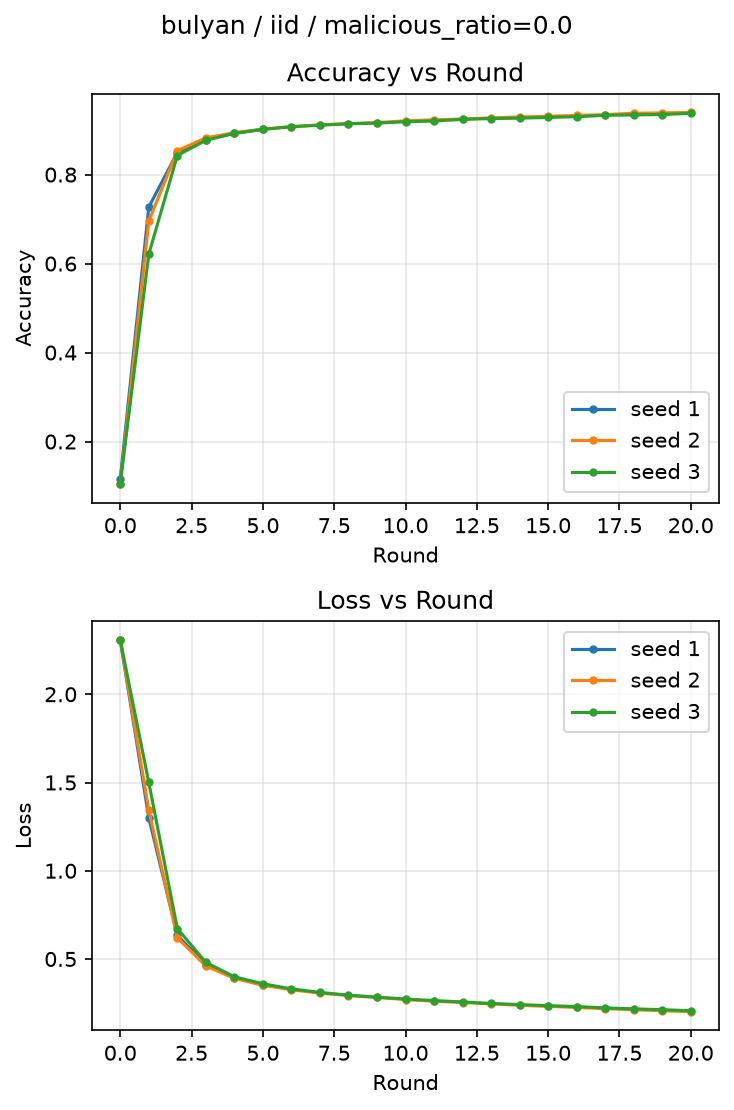
\includegraphics[width=\columnwidth]{seed_curves_bulyan_iid_ratio0.0.png}
    \caption{Seed ごとの Round-Accuracy および Round-Loss の推移（IID，悪性クライアント比率 0.0）}
    \label{fig:seed_curves_bulyan_iid_ratio0.0}
\end{figure}
% =========================================================
\subsubsection{結果}
% =========================================================

表\ref{tab:bulyan_iid_ratio0.0}に，各ラウンドにおける
Accuracy および Loss を示す．

学習開始時（Round 0）の Accuracy は約 0.1042--0.1163 であったが，Round 1 では約 0.6211--0.7270 まで上昇した． その後も学習ラウンドの進行に伴って Accuracy は継続的に向上し，Round 20 ではすべての Seed において約 0.9377--0.9398 に達した． Round 20 時点の Loss は約 0.2016--0.2069 であった．

なお，Seed 1（Round 5 まで） は Round 20 到達前にログが途切れており，実験が途中で終了したものと考えられる（原因不明のため，欠損箇所は表中で「--」と表記した）．

\clearpage
% =========================================================
\subsection{Bulyan：IID・悪性クライアント比率 0.1}
% =========================================================

\subsubsection{実験条件}

\begin{itemize}
    \item \textbf{Aggregation method:} Bulyan
    \item \textbf{Data split:} IID
    \item \textbf{Malicious ratio:} 0.1
    \item \textbf{Attack:} Adaptive attack
    \item \textbf{Number of rounds:} 20
    \item \textbf{Seeds:} 1, 2, 3
\end{itemize}

% =========================================================
% 実験結果表
% =========================================================

\begin{table}[H]
\centering

\caption{Bulyan（IID，悪性クライアント比率 0.1）における
Accuracy および Loss}

\label{tab:bulyan_iid_ratio0.1}

\footnotesize
\setlength{\tabcolsep}{2.5pt}
\renewcommand{\arraystretch}{0.90}

\resizebox{\columnwidth}{!}{%
\begin{tabular}{c cc cc cc}

\toprule

& \multicolumn{2}{c}{Seed 1}
& \multicolumn{2}{c}{Seed 2}
& \multicolumn{2}{c}{Seed 3} \\

\cmidrule(lr){2-3}
\cmidrule(lr){4-5}
\cmidrule(lr){6-7}

Round
& Acc. & Loss
& Acc. & Loss
& Acc. & Loss \\

\midrule

0 & 0.1161 & 2.3144 & 0.1072 & 2.3135 & 0.1142 & 2.3133 \\
1 & 0.6630 & 1.4685 & 0.6822 & 1.5466 & 0.7033 & 1.5352 \\
2 & 0.8283 & 0.7152 & 0.8259 & 0.7232 & 0.8253 & 0.7152 \\
3 & 0.8706 & 0.5232 & 0.8637 & 0.5270 & 0.8639 & 0.5235 \\
4 & 0.8844 & 0.4398 & 0.8802 & 0.4417 & 0.8834 & 0.4375 \\
5 & 0.8914 & 0.3910 & 0.8922 & 0.3941 & 0.8928 & 0.3890 \\
6 & 0.8986 & 0.3615 & 0.8976 & 0.3626 & 0.9005 & 0.3585 \\
7 & 0.9040 & 0.3409 & 0.9033 & 0.3408 & 0.9039 & 0.3384 \\
8 & 0.9070 & 0.3248 & 0.9073 & 0.3242 & 0.9074 & 0.3240 \\
9 & 0.9106 & 0.3113 & 0.9106 & 0.3100 & 0.9102 & 0.3116 \\
10 & 0.9131 & 0.3001 & 0.9133 & 0.3002 & 0.9133 & 0.2997 \\
11 & 0.9154 & 0.2911 & 0.9163 & 0.2906 & 0.9153 & 0.2911 \\
12 & 0.9162 & 0.2832 & 0.9179 & 0.2827 & 0.9171 & 0.2836 \\
13 & 0.9177 & 0.2757 & 0.9181 & 0.2763 & 0.9180 & 0.2771 \\
14 & 0.9197 & 0.2696 & 0.9207 & 0.2695 & 0.9196 & 0.2711 \\
15 & 0.9206 & 0.2648 & 0.9219 & 0.2638 & 0.9221 & 0.2645 \\
16 & 0.9214 & 0.2602 & 0.9239 & 0.2584 & 0.9228 & 0.2592 \\
17 & 0.9239 & 0.2547 & 0.9249 & 0.2543 & 0.9238 & 0.2548 \\
18 & 0.9253 & 0.2495 & 0.9266 & 0.2494 & 0.9249 & 0.2501 \\
19 & 0.9261 & 0.2456 & 0.9273 & 0.2458 & 0.9260 & 0.2461 \\
20 & 0.9273 & 0.2413 & 0.9290 & 0.2413 & 0.9266 & 0.2431 \\

\bottomrule

\end{tabular}%
}

\end{table}
\begin{figure}[H]
    \centering
    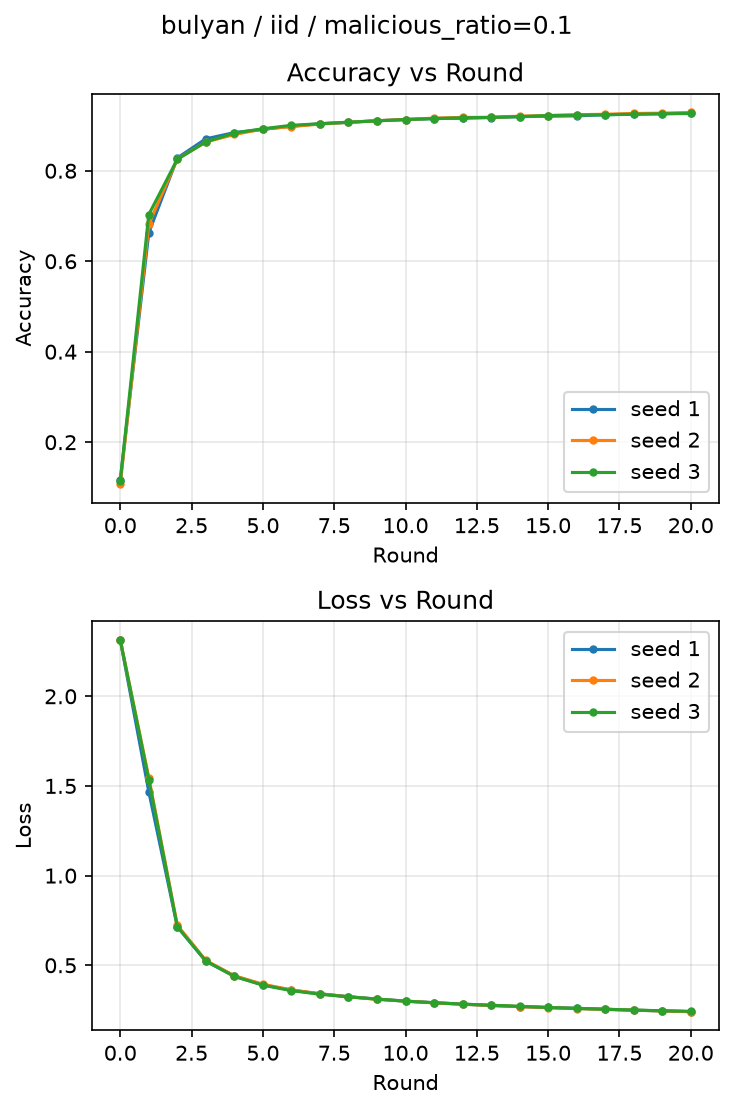
\includegraphics[width=\columnwidth]{seed_curves_bulyan_iid_ratio0.1.png}
    \caption{Seed ごとの Round-Accuracy および Round-Loss の推移（IID，悪性クライアント比率 0.1）}
    \label{fig:seed_curves_bulyan_iid_ratio0.1}
\end{figure}
% =========================================================
\subsubsection{結果}
% =========================================================

表\ref{tab:bulyan_iid_ratio0.1}に，各ラウンドにおける
Accuracy および Loss を示す．

学習開始時（Round 0）の Accuracy は約 0.1072--0.1161 であったが，Round 1 では約 0.6630--0.7033 まで上昇した． その後も学習ラウンドの進行に伴って Accuracy は継続的に向上し，Round 20 ではすべての Seed において約 0.9266--0.9290 に達した． Round 20 時点の Loss は約 0.2413--0.2431 であった． 悪性クライアント比率 0.0 の場合（最終 Accuracy 平均 約 0.9387）と比較しても最終的な Accuracy に大きな差は見られず，本条件下でも学習は概ね安定していたといえる．

\clearpage
% =========================================================
\subsection{Bulyan：IID・悪性クライアント比率 0.2}
% =========================================================

\subsubsection{実験条件}

\begin{itemize}
    \item \textbf{Aggregation method:} Bulyan
    \item \textbf{Data split:} IID
    \item \textbf{Malicious ratio:} 0.2
    \item \textbf{Attack:} Adaptive attack
    \item \textbf{Number of rounds:} 20
    \item \textbf{Seeds:} 1, 2, 3
\end{itemize}

% =========================================================
% 実験結果表
% =========================================================

\begin{table}[H]
\centering

\caption{Bulyan（IID，悪性クライアント比率 0.2）における
Accuracy および Loss}

\label{tab:bulyan_iid_ratio0.2}

\footnotesize
\setlength{\tabcolsep}{2.5pt}
\renewcommand{\arraystretch}{0.90}

\resizebox{\columnwidth}{!}{%
\begin{tabular}{c cc cc cc}

\toprule

& \multicolumn{2}{c}{Seed 1}
& \multicolumn{2}{c}{Seed 2}
& \multicolumn{2}{c}{Seed 3} \\

\cmidrule(lr){2-3}
\cmidrule(lr){4-5}
\cmidrule(lr){6-7}

Round
& Acc. & Loss
& Acc. & Loss
& Acc. & Loss \\

\midrule

0 & 0.0896 & 2.3146 & 0.1170 & 2.3013 & 0.1022 & 2.3042 \\
1 & 0.6866 & 1.5967 & 0.6131 & 1.5577 & 0.6801 & 1.7182 \\
2 & 0.8214 & 0.8490 & 0.8278 & 0.8252 & 0.8206 & 0.8691 \\
3 & 0.8512 & 0.6254 & 0.8593 & 0.5994 & 0.8573 & 0.6139 \\
4 & 0.8694 & 0.5284 & 0.8763 & 0.5090 & 0.8752 & 0.5124 \\
5 & 0.8788 & 0.4752 & 0.8851 & 0.4606 & 0.8854 & 0.4600 \\
6 & 0.8855 & 0.4412 & 0.8885 & 0.4315 & 0.8895 & 0.4294 \\
7 & 0.8892 & 0.4205 & 0.8899 & 0.4142 & 0.8910 & 0.4124 \\
8 & 0.8931 & 0.4029 & 0.8940 & 0.3995 & 0.8957 & 0.3917 \\
9 & 0.8931 & 0.3930 & 0.8961 & 0.3891 & 0.8975 & 0.3835 \\
10 & 0.8939 & 0.3870 & 0.8965 & 0.3812 & 0.8985 & 0.3746 \\
11 & 0.8957 & 0.3800 & 0.8963 & 0.3750 & 0.9002 & 0.3703 \\
12 & 0.8970 & 0.3743 & 0.8972 & 0.3686 & 0.8980 & 0.3694 \\
13 & 0.8979 & 0.3694 & 0.8961 & 0.3653 & 0.8987 & 0.3659 \\
14 & 0.8985 & 0.3669 & 0.8987 & 0.3600 & 0.8987 & 0.3620 \\
15 & 0.8965 & 0.3660 & 0.9000 & 0.3557 & 0.9000 & 0.3568 \\
16 & 0.8999 & 0.3597 & 0.9006 & 0.3531 & 0.9012 & 0.3534 \\
17 & 0.8992 & 0.3573 & 0.9018 & 0.3509 & 0.9006 & 0.3517 \\
18 & 0.9005 & 0.3534 & 0.9020 & 0.3485 & 0.9019 & 0.3479 \\
19 & 0.8996 & 0.3514 & 0.9033 & 0.3472 & 0.8999 & 0.3471 \\
20 & 0.8995 & 0.3523 & 0.9019 & 0.3453 & 0.9012 & 0.3459 \\

\bottomrule

\end{tabular}%
}

\end{table}
\begin{figure}[H]
    \centering
    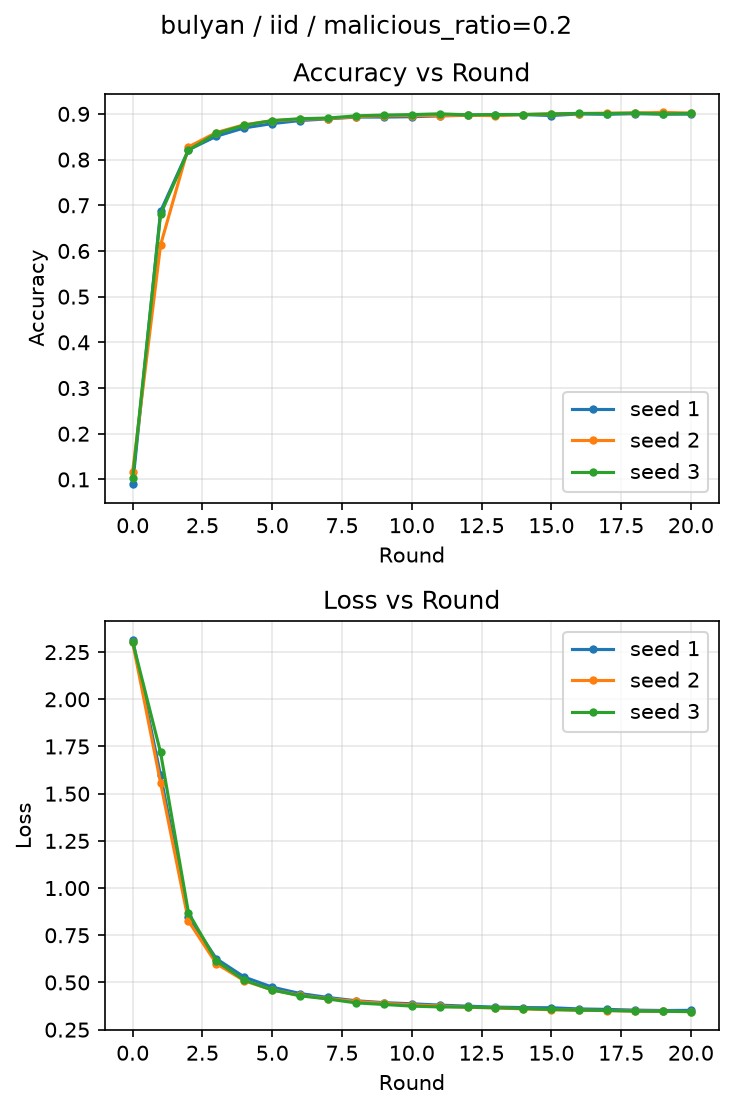
\includegraphics[width=\columnwidth]{seed_curves_bulyan_iid_ratio0.2.png}
    \caption{Seed ごとの Round-Accuracy および Round-Loss の推移（IID，悪性クライアント比率 0.2）}
    \label{fig:seed_curves_bulyan_iid_ratio0.2}
\end{figure}
% =========================================================
\subsubsection{結果}
% =========================================================

表\ref{tab:bulyan_iid_ratio0.2}に，各ラウンドにおける
Accuracy および Loss を示す．

学習開始時（Round 0）の Accuracy は約 0.0896--0.1170 であったが，Round 1 では約 0.6131--0.6866 まで上昇した． その後も学習ラウンドの進行に伴って Accuracy は継続的に向上し，Round 20 ではすべての Seed において約 0.8995--0.9019 に達した． Round 20 時点の Loss は約 0.3453--0.3523 であった． 悪性クライアント比率 0.0 の場合（最終 Accuracy 平均 約 0.9387）と比較すると，本条件では約 0.0379 ポイント低い水準にとどまっており，悪性クライアント比率 0.2 における攻撃の影響が最終的な Accuracy にも現れていることが分かる．

\clearpage
% =========================================================
\subsection{Bulyan：IID・悪性クライアント比率 0.3}
% =========================================================

\subsubsection{実験条件}

\begin{itemize}
    \item \textbf{Aggregation method:} Bulyan
    \item \textbf{Data split:} IID
    \item \textbf{Malicious ratio:} 0.3
    \item \textbf{Attack:} Adaptive attack
    \item \textbf{Number of rounds:} 20
    \item \textbf{Seeds:} 1, 2, 3
\end{itemize}

\subsubsection{結果}

悪性クライアント比率 0.3（クライアント数 100，悪性クライアント数 $f=30$）の条件では，Bulyan の頑健性条件（$n \geq 4f+3$）を満たさず（$100 < 4 \times 30 + 3 = 123$），Round 0 の初期評価以降に学習が破綻し，Round 1 以降のログが記録されなかった．そのため本条件については表・図による詳細な報告を省略する．

\clearpage
% =========================================================
\subsection{Bulyan：IID・悪性クライアント比率別の比較（Seed平均）}
% =========================================================

\subsubsection{実験条件}

\begin{itemize}
    \item \textbf{Aggregation method:} Bulyan
    \item \textbf{Data split:} IID
    \item \textbf{Malicious ratio:} 0.0, 0.1, 0.2
    \item \textbf{Attack:} Adaptive attack
    \item \textbf{Number of rounds:} 20
    \item \textbf{Seeds:} 1, 2, 3（平均 $\pm$ 標準偏差）
\end{itemize}

9.4 節で述べたとおり，malicious ratio 0.3（$f=30$）は Bulyan の
頑健性条件 $n \geq 4f+3$（$100 < 123$）を満たさず，Round 0 以降の
ログが存在しないため，本節の malicious ratio 別比較には
malicious ratio 0.0, 0.1, 0.2（いずれも $n \geq 4f+3$ を満たす）
のみを対象とする．
図の作成には \verb|result/plot_seed_mean_by_ratio.py| を
\verb|--aggregation bulyan --split iid --ratios 0.0,0.1,0.2| オプ
ションで用い，\verb|result/results.csv| から Bulyan・IID の条件に
一致する run を malicious ratio ごとに抽出し，ラウンドごとの
平均・標準偏差を計算して描画した．

% =========================================================
% 実験結果図
% =========================================================

\begin{figure}[H]
    \centering
    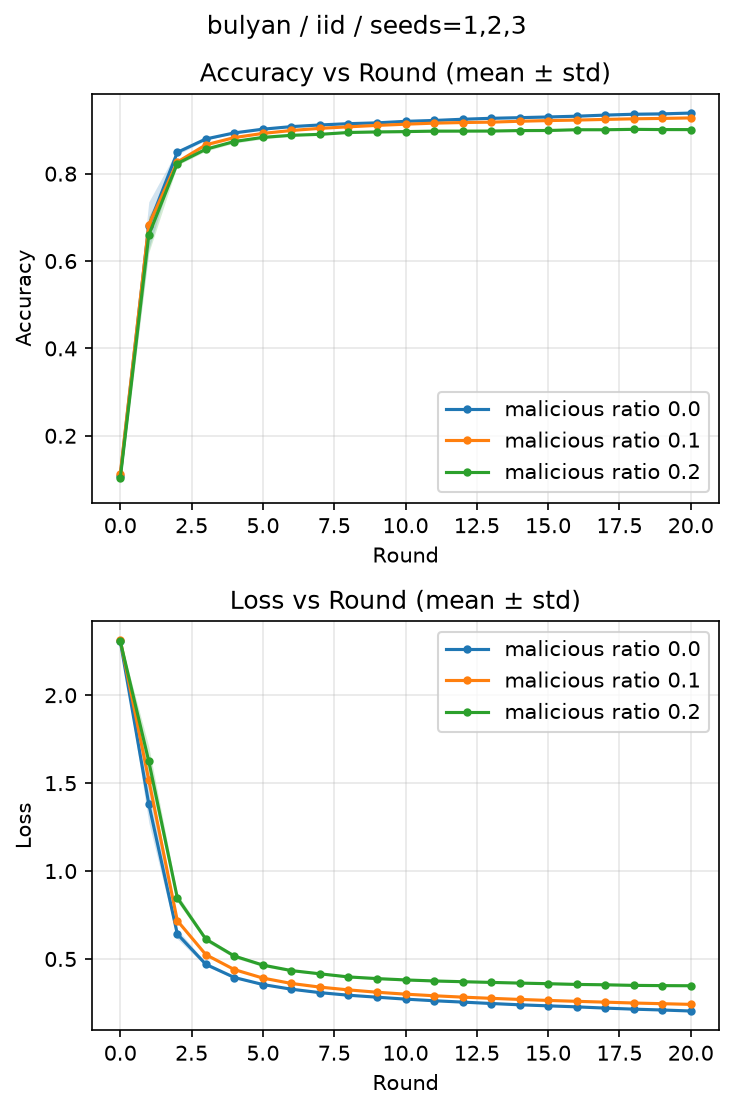
\includegraphics[width=\columnwidth]{bulyan_iid_seedmean_by_ratio.png}
    \caption{Bulyan・IID における malicious ratio 別の
    Round-Accuracy および Round-Loss の推移（Seed 平均 $\pm$
    標準偏差，malicious ratio 0.3 は頑健性条件を満たさないため
    対象外）}
    \label{fig:bulyan_iid_seedmean_by_ratio}
\end{figure}

% =========================================================
\subsubsection{結果}
% =========================================================

図\ref{fig:bulyan_iid_seedmean_by_ratio}に，malicious ratio
0.0, 0.1, 0.2 における Round-Accuracy および Round-Loss の
平均 $\pm$ 標準偏差の推移を示す．

Round 20 時点の平均 Accuracy（標準偏差）は，malicious ratio 0.0 で
0.9388（0.0015），ratio 0.1 で 0.9276（0.0012），ratio 0.2 で
0.9009（0.0012）であり，いずれの malicious ratio でも標準偏差は
0.002 未満と極めて小さく，図上でも帯はほとんど視認できない．
Loss についても malicious ratio 0.0 で 0.2042，ratio 0.1 で
0.2419，ratio 0.2 で 0.3478 と穏やかに増加するのみであり，
6--8 章で見られたような malicious ratio に伴う Seed 間の
ばらつき拡大は，頑健性条件を満たす範囲では確認されなかった。

以上より，Bulyan は頑健性条件 $n \geq 4f+3$ を満たす
malicious ratio 0.0--0.2 の範囲では，Accuracy・Loss ともに
Seed 間の再現性が高く安定した学習が可能である一方，
条件を満たさない malicious ratio 0.3 では学習そのものが
破綻するという二極化した挙動を示すことが確認された．

\clearpage
% =========================================================
\section{Bulyan（Non-IID環境）における悪性クライアント比率別の評価}
% =========================================================

% =========================================================
\subsection{Bulyan：Non-IID・悪性クライアント比率 0.0}
% =========================================================

\subsubsection{実験条件}

\begin{itemize}
    \item \textbf{Aggregation method:} Bulyan
    \item \textbf{Data split:} Non-IID
    \item \textbf{Malicious ratio:} 0.0
    \item \textbf{Attack:} Adaptive attack
    \item \textbf{Number of rounds:} 20
    \item \textbf{Seeds:} 1, 2, 3
\end{itemize}

% =========================================================
% 実験結果表
% =========================================================

\begin{table}[H]
\centering

\caption{Bulyan（Non-IID，悪性クライアント比率 0.0）における
Accuracy および Loss}

\label{tab:bulyan_non_iid_ratio0.0}

\footnotesize
\setlength{\tabcolsep}{2.5pt}
\renewcommand{\arraystretch}{0.90}

\resizebox{\columnwidth}{!}{%
\begin{tabular}{c cc cc cc}

\toprule

& \multicolumn{2}{c}{Seed 1}
& \multicolumn{2}{c}{Seed 2}
& \multicolumn{2}{c}{Seed 3} \\

\cmidrule(lr){2-3}
\cmidrule(lr){4-5}
\cmidrule(lr){6-7}

Round
& Acc. & Loss
& Acc. & Loss
& Acc. & Loss \\

\midrule

0 & 0.1208 & 2.3094 & 0.1155 & 2.3121 & 0.0912 & 2.3195 \\
1 & 0.6626 & 1.6723 & 0.6795 & 1.7022 & 0.6118 & 1.6819 \\
2 & 0.8161 & 0.9203 & 0.7724 & 0.9725 & 0.8076 & 0.9103 \\
3 & 0.8534 & 0.6223 & 0.8493 & 0.6600 & 0.8513 & 0.6309 \\
4 & 0.8757 & 0.4996 & 0.8725 & 0.5194 & 0.8740 & 0.5057 \\
5 & 0.8889 & 0.4318 & 0.8838 & 0.4438 & 0.8854 & 0.4357 \\
6 & 0.8975 & 0.3915 & 0.8940 & 0.3964 & 0.8919 & 0.3939 \\
7 & 0.9029 & 0.3594 & 0.9002 & 0.3625 & 0.8974 & 0.3656 \\
8 & 0.9064 & 0.3397 & 0.9042 & 0.3413 & 0.9023 & 0.3445 \\
9 & 0.9097 & 0.3213 & 0.9076 & 0.3234 & 0.9070 & 0.3274 \\
10 & 0.9133 & 0.3065 & 0.9115 & 0.3077 & 0.9101 & 0.3140 \\
11 & 0.9148 & 0.2954 & 0.9146 & 0.2949 & 0.9119 & 0.3033 \\
12 & 0.9172 & 0.2843 & 0.9155 & 0.2843 & 0.9142 & 0.2931 \\
13 & 0.9192 & 0.2763 & 0.9185 & 0.2760 & 0.9161 & 0.2846 \\
14 & 0.9210 & 0.2677 & 0.9203 & 0.2658 & 0.9181 & 0.2770 \\
15 & 0.9230 & 0.2594 & 0.9218 & 0.2603 & 0.9192 & 0.2697 \\
16 & 0.9248 & 0.2513 & 0.9237 & 0.2524 & 0.9206 & 0.2641 \\
17 & 0.9255 & 0.2456 & 0.9260 & 0.2458 & 0.9219 & 0.2575 \\
18 & 0.9277 & 0.2382 & 0.9276 & 0.2392 & 0.9239 & 0.2522 \\
19 & 0.9297 & 0.2326 & 0.9297 & 0.2332 & 0.9252 & 0.2460 \\
20 & 0.9301 & 0.2274 & 0.9319 & 0.2280 & 0.9266 & 0.2422 \\

\bottomrule

\end{tabular}%
}

\end{table}
\begin{figure}[H]
    \centering
    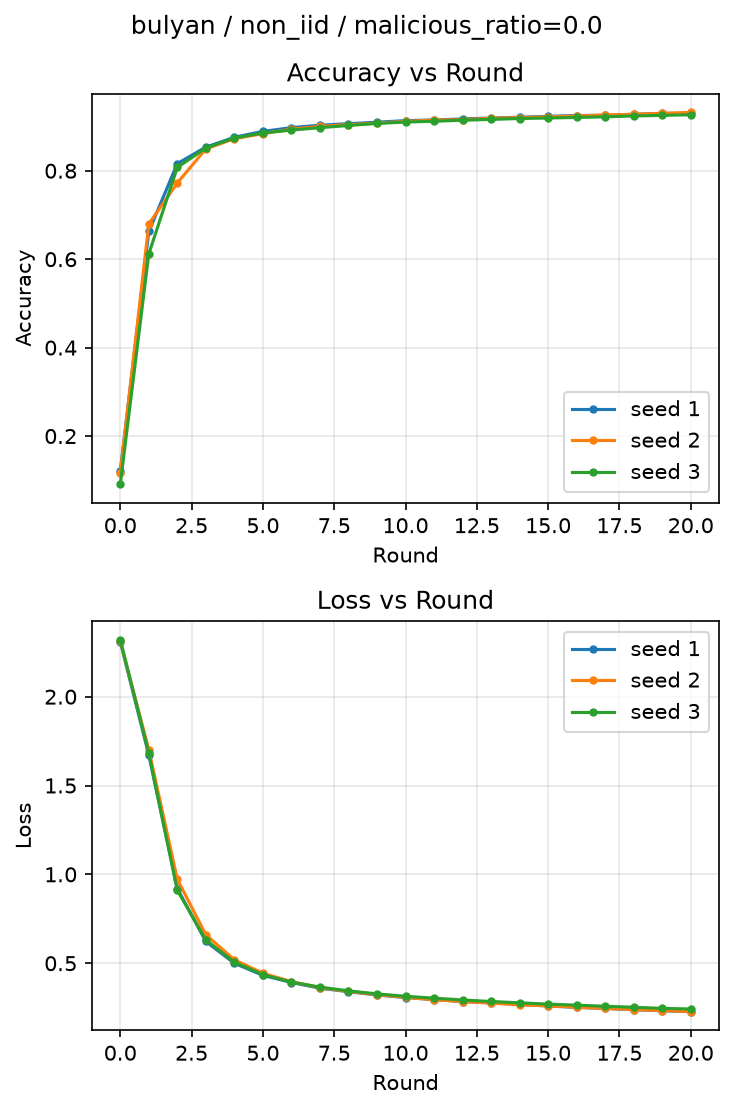
\includegraphics[width=\columnwidth]{seed_curves_bulyan_non_iid_ratio0.0.png}
    \caption{Seed ごとの Round-Accuracy および Round-Loss の推移（Non-IID，悪性クライアント比率 0.0）}
    \label{fig:seed_curves_bulyan_non_iid_ratio0.0}
\end{figure}
% =========================================================
\subsubsection{結果}
% =========================================================

表\ref{tab:bulyan_non_iid_ratio0.0}に，各ラウンドにおける
Accuracy および Loss を示す．

学習開始時（Round 0）の Accuracy は約 0.0912--0.1208 であったが，Round 1 では約 0.6118--0.6795 まで上昇した． その後も学習ラウンドの進行に伴って Accuracy は継続的に向上し，Round 20 ではすべての Seed において約 0.9266--0.9319 に達した． Round 20 時点の Loss は約 0.2274--0.2422 であった．

\clearpage
% =========================================================
\subsection{Bulyan：Non-IID・悪性クライアント比率 0.1}
% =========================================================

\subsubsection{実験条件}

\begin{itemize}
    \item \textbf{Aggregation method:} Bulyan
    \item \textbf{Data split:} Non-IID
    \item \textbf{Malicious ratio:} 0.1
    \item \textbf{Attack:} Adaptive attack
    \item \textbf{Number of rounds:} 20
    \item \textbf{Seeds:} 1, 2, 3
\end{itemize}

% =========================================================
% 実験結果表
% =========================================================

\begin{table}[H]
\centering

\caption{Bulyan（Non-IID，悪性クライアント比率 0.1）における
Accuracy および Loss}

\label{tab:bulyan_non_iid_ratio0.1}

\footnotesize
\setlength{\tabcolsep}{2.5pt}
\renewcommand{\arraystretch}{0.90}

\resizebox{\columnwidth}{!}{%
\begin{tabular}{c cc cc cc}

\toprule

& \multicolumn{2}{c}{Seed 1}
& \multicolumn{2}{c}{Seed 2}
& \multicolumn{2}{c}{Seed 3} \\

\cmidrule(lr){2-3}
\cmidrule(lr){4-5}
\cmidrule(lr){6-7}

Round
& Acc. & Loss
& Acc. & Loss
& Acc. & Loss \\

\midrule

0 & 0.1520 & 2.2996 & 0.1104 & 2.3111 & 0.1265 & 2.3120 \\
1 & 0.5413 & 1.7702 & 0.5897 & 1.8200 & 0.5531 & 1.8307 \\
2 & 0.7377 & 1.1684 & 0.7712 & 1.0723 & 0.7573 & 1.1531 \\
3 & 0.8142 & 0.8240 & 0.8342 & 0.7388 & 0.8225 & 0.7964 \\
4 & 0.8525 & 0.6392 & 0.8605 & 0.5837 & 0.8493 & 0.6217 \\
5 & 0.8695 & 0.5357 & 0.8747 & 0.5018 & 0.8698 & 0.5191 \\
6 & 0.8842 & 0.4688 & 0.8833 & 0.4470 & 0.8786 & 0.4604 \\
7 & 0.8883 & 0.4288 & 0.8916 & 0.4109 & 0.8859 & 0.4212 \\
8 & 0.8937 & 0.3970 & 0.8980 & 0.3836 & 0.8932 & 0.3905 \\
9 & 0.8981 & 0.3744 & 0.9003 & 0.3680 & 0.8994 & 0.3679 \\
10 & 0.8999 & 0.3593 & 0.9037 & 0.3509 & 0.9038 & 0.3485 \\
11 & 0.9016 & 0.3469 & 0.9059 & 0.3374 & 0.9052 & 0.3350 \\
12 & 0.9045 & 0.3344 & 0.9084 & 0.3281 & 0.9071 & 0.3237 \\
13 & 0.9065 & 0.3245 & 0.9098 & 0.3177 & 0.9087 & 0.3151 \\
14 & 0.9087 & 0.3158 & 0.9113 & 0.3101 & 0.9123 & 0.3035 \\
15 & 0.9100 & 0.3087 & 0.9122 & 0.3039 & 0.9120 & 0.2983 \\
16 & 0.9123 & 0.3019 & 0.9138 & 0.2968 & 0.9151 & 0.2910 \\
17 & 0.9133 & 0.2983 & 0.9155 & 0.2887 & 0.9167 & 0.2844 \\
18 & 0.9138 & 0.2925 & 0.9162 & 0.2859 & 0.9180 & 0.2778 \\
19 & 0.9152 & 0.2877 & 0.9175 & 0.2822 & 0.9187 & 0.2742 \\
20 & 0.9153 & 0.2849 & 0.9170 & 0.2775 & 0.9198 & 0.2702 \\

\bottomrule

\end{tabular}%
}

\end{table}
\begin{figure}[H]
    \centering
    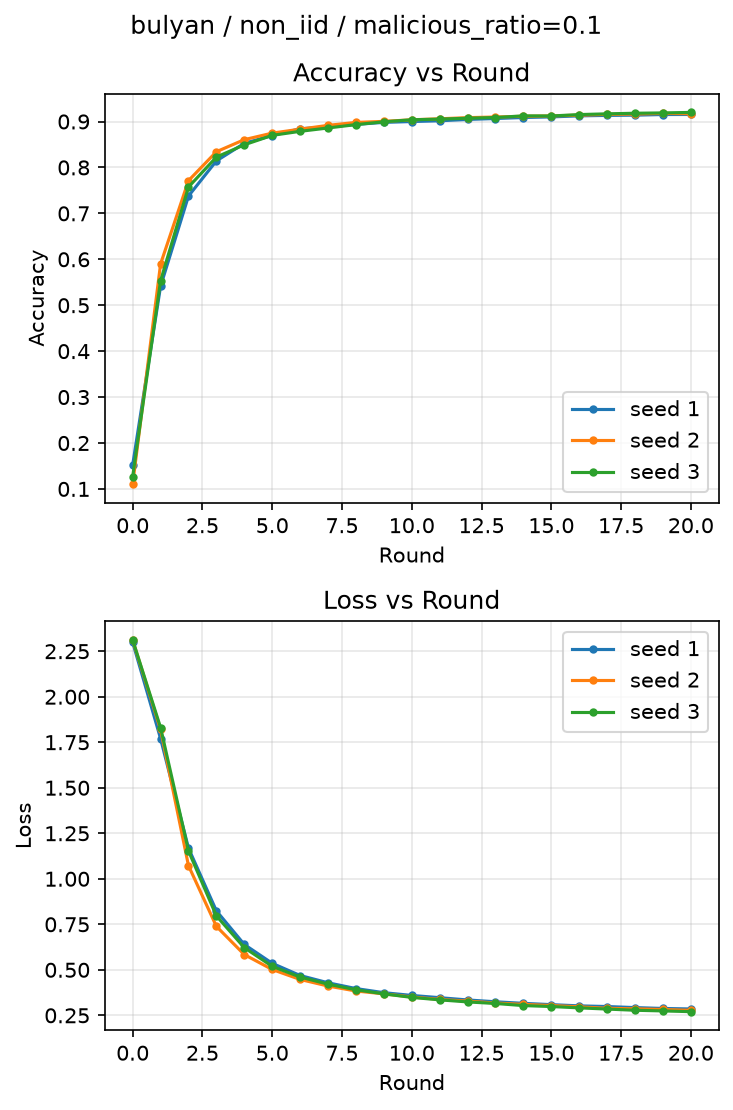
\includegraphics[width=\columnwidth]{seed_curves_bulyan_non_iid_ratio0.1.png}
    \caption{Seed ごとの Round-Accuracy および Round-Loss の推移（Non-IID，悪性クライアント比率 0.1）}
    \label{fig:seed_curves_bulyan_non_iid_ratio0.1}
\end{figure}
% =========================================================
\subsubsection{結果}
% =========================================================

表\ref{tab:bulyan_non_iid_ratio0.1}に，各ラウンドにおける
Accuracy および Loss を示す．

学習開始時（Round 0）の Accuracy は約 0.1104--0.1520 であったが，Round 1 では約 0.5413--0.5897 まで上昇した． その後も学習ラウンドの進行に伴って Accuracy は継続的に向上し，Round 20 ではすべての Seed において約 0.9153--0.9198 に達した． Round 20 時点の Loss は約 0.2702--0.2849 であった． 悪性クライアント比率 0.0 の場合（最終 Accuracy 平均 約 0.9295）と比較しても最終的な Accuracy に大きな差は見られず，本条件下でも学習は概ね安定していたといえる．

\clearpage
% =========================================================
\subsection{Bulyan：Non-IID・悪性クライアント比率 0.2}
% =========================================================

\subsubsection{実験条件}

\begin{itemize}
    \item \textbf{Aggregation method:} Bulyan
    \item \textbf{Data split:} Non-IID
    \item \textbf{Malicious ratio:} 0.2
    \item \textbf{Attack:} Adaptive attack
    \item \textbf{Number of rounds:} 20
    \item \textbf{Seeds:} 1, 2, 3
\end{itemize}

% =========================================================
% 実験結果表
% =========================================================

\begin{table}[H]
\centering

\caption{Bulyan（Non-IID，悪性クライアント比率 0.2）における
Accuracy および Loss}

\label{tab:bulyan_non_iid_ratio0.2}

\footnotesize
\setlength{\tabcolsep}{2.5pt}
\renewcommand{\arraystretch}{0.90}

\resizebox{\columnwidth}{!}{%
\begin{tabular}{c cc cc cc}

\toprule

& \multicolumn{2}{c}{Seed 1}
& \multicolumn{2}{c}{Seed 2}
& \multicolumn{2}{c}{Seed 3} \\

\cmidrule(lr){2-3}
\cmidrule(lr){4-5}
\cmidrule(lr){6-7}

Round
& Acc. & Loss
& Acc. & Loss
& Acc. & Loss \\

\midrule

0 & 0.1071 & 2.3116 & 0.1094 & 2.3124 & 0.0547 & 2.3126 \\
1 & 0.4346 & 2.1531 & 0.3580 & 2.0922 & 0.3704 & 2.1129 \\
2 & 0.5855 & 1.8393 & 0.6035 & 1.6792 & 0.5710 & 1.7678 \\
3 & 0.6556 & 1.4864 & 0.6945 & 1.3181 & 0.6746 & 1.4229 \\
4 & 0.7108 & 1.2065 & 0.7382 & 1.0951 & 0.7596 & 1.1412 \\
5 & 0.7258 & 1.0304 & 0.7658 & 0.9519 & 0.8028 & 0.9508 \\
6 & 0.7567 & 0.8933 & 0.7963 & 0.8464 & 0.8284 & 0.8289 \\
7 & 0.7590 & 0.8282 & 0.8075 & 0.7767 & 0.8352 & 0.7574 \\
8 & 0.7754 & 0.7723 & 0.8137 & 0.7324 & 0.8418 & 0.6969 \\
9 & 0.7764 & 0.7421 & 0.8201 & 0.6929 & 0.8478 & 0.6523 \\
10 & 0.7922 & 0.6964 & 0.8209 & 0.6682 & 0.8543 & 0.6187 \\
11 & 0.8016 & 0.6712 & 0.8126 & 0.6596 & 0.8520 & 0.6130 \\
12 & 0.8033 & 0.6596 & 0.8239 & 0.6454 & 0.8561 & 0.5907 \\
13 & 0.8047 & 0.6462 & 0.8258 & 0.6332 & 0.8558 & 0.5869 \\
14 & 0.8127 & 0.6286 & 0.8260 & 0.6234 & 0.8578 & 0.5765 \\
15 & 0.8086 & 0.6268 & 0.8210 & 0.6175 & 0.8585 & 0.5709 \\
16 & 0.8102 & 0.6196 & 0.8264 & 0.6044 & 0.8637 & 0.5574 \\
17 & 0.8064 & 0.6196 & 0.8342 & 0.5956 & 0.8594 & 0.5668 \\
18 & 0.8037 & 0.6210 & 0.8248 & 0.6006 & 0.8584 & 0.5563 \\
19 & 0.8107 & 0.6083 & 0.8268 & 0.5911 & 0.8596 & 0.5593 \\
20 & 0.8102 & 0.6032 & 0.8273 & 0.5878 & 0.8621 & 0.5450 \\

\bottomrule

\end{tabular}%
}

\end{table}
\begin{figure}[H]
    \centering
    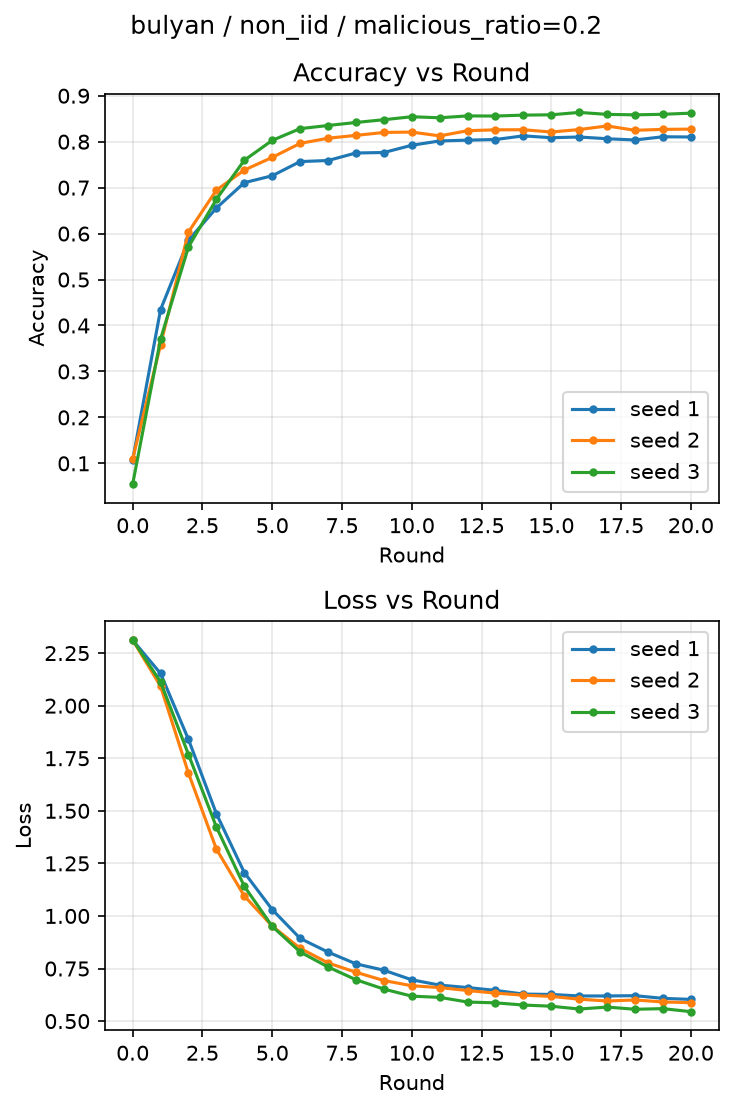
\includegraphics[width=\columnwidth]{seed_curves_bulyan_non_iid_ratio0.2.png}
    \caption{Seed ごとの Round-Accuracy および Round-Loss の推移（Non-IID，悪性クライアント比率 0.2）}
    \label{fig:seed_curves_bulyan_non_iid_ratio0.2}
\end{figure}
% =========================================================
\subsubsection{結果}
% =========================================================

表\ref{tab:bulyan_non_iid_ratio0.2}に，各ラウンドにおける
Accuracy および Loss を示す．

学習開始時（Round 0）の Accuracy は約 0.0547--0.1094 であったが，Round 1 では約 0.3580--0.4346 まで上昇した． その後も学習ラウンドの進行に伴って Accuracy は継続的に向上し，Round 20 ではすべての Seed において約 0.8102--0.8621 に達した． Round 20 時点の Loss は約 0.5450--0.6032 であった． 悪性クライアント比率 0.0 の場合（最終 Accuracy 平均 約 0.9295）と比較すると，本条件では約 0.0963 ポイント低い水準にとどまっており，悪性クライアント比率 0.2 における攻撃の影響が最終的な Accuracy にも現れていることが分かる．

\clearpage
% =========================================================
\subsection{Bulyan：Non-IID・悪性クライアント比率 0.3}
% =========================================================

\subsubsection{実験条件}

\begin{itemize}
    \item \textbf{Aggregation method:} Bulyan
    \item \textbf{Data split:} Non-IID
    \item \textbf{Malicious ratio:} 0.3
    \item \textbf{Attack:} Adaptive attack
    \item \textbf{Number of rounds:} 20
    \item \textbf{Seeds:} 1, 2, 3
\end{itemize}

\subsubsection{結果}

悪性クライアント比率 0.3（クライアント数 100，悪性クライアント数 $f=30$）の条件では，Bulyan の頑健性条件（$n \geq 4f+3$）を満たさず（$100 < 4 \times 30 + 3 = 123$），Round 0 の初期評価以降に学習が破綻し，Round 1 以降のログが記録されなかった．そのため本条件については表・図による詳細な報告を省略する．

\clearpage
% =========================================================
\subsection{Bulyan：Non-IID・悪性クライアント比率別の比較（Seed平均）}
% =========================================================

\subsubsection{実験条件}

\begin{itemize}
    \item \textbf{Aggregation method:} Bulyan
    \item \textbf{Data split:} Non-IID
    \item \textbf{Malicious ratio:} 0.0, 0.1, 0.2
    \item \textbf{Attack:} Adaptive attack
    \item \textbf{Number of rounds:} 20
    \item \textbf{Seeds:} 1, 2, 3（平均 $\pm$ 標準偏差）
\end{itemize}

9.5 節（Bulyan・IID）と同様に，malicious ratio 0.3 は頑健性条件
$n \geq 4f+3$（$100 < 123$）を満たさず Round 0 以降のログが
存在しないため，本節でも malicious ratio 0.0, 0.1, 0.2 のみを
比較対象とする．
図の作成には \verb|result/plot_seed_mean_by_ratio.py| を
\verb|--aggregation bulyan --split non_iid --ratios 0.0,0.1,0.2|
オプションで用い，\verb|result/results.csv| から Bulyan・Non-IID
の条件に一致する run を malicious ratio ごとに抽出し，
ラウンドごとの平均・標準偏差を計算して描画した．

% =========================================================
% 実験結果図
% =========================================================

\begin{figure}[H]
    \centering
    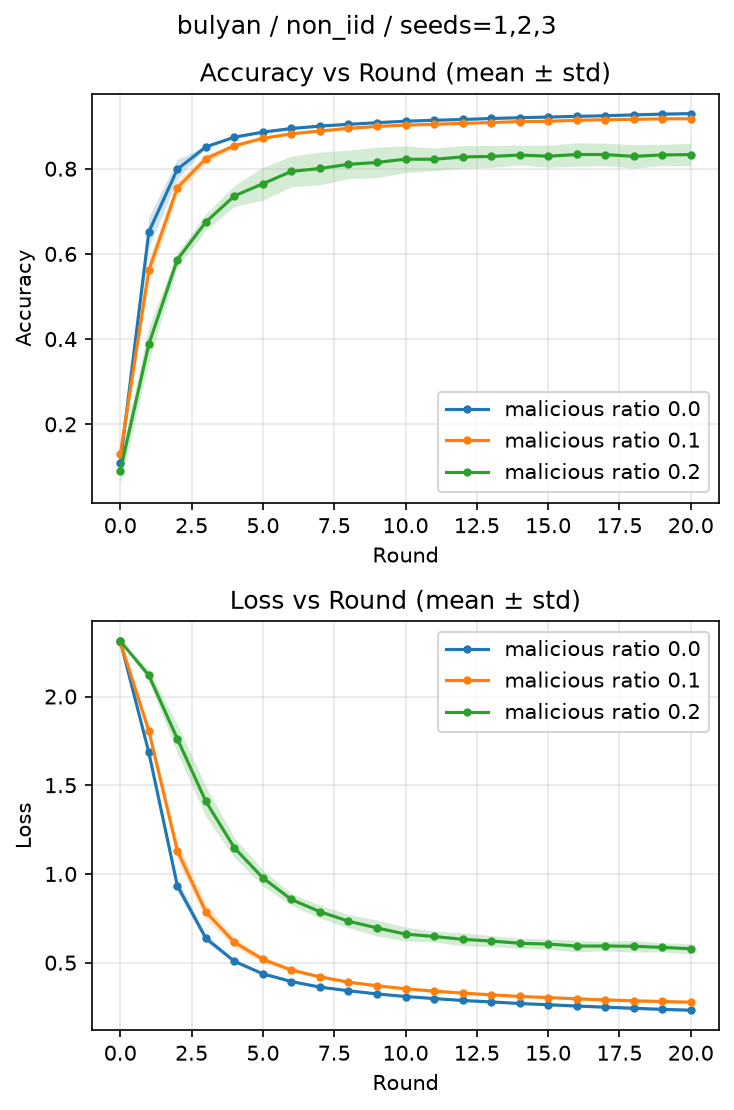
\includegraphics[width=\columnwidth]{bulyan_noniid_seedmean_by_ratio.png}
    \caption{Bulyan・Non-IID における malicious ratio 別の
    Round-Accuracy および Round-Loss の推移（Seed 平均 $\pm$
    標準偏差，malicious ratio 0.3 は頑健性条件を満たさないため
    対象外）}
    \label{fig:bulyan_noniid_seedmean_by_ratio}
\end{figure}

% =========================================================
\subsubsection{結果}
% =========================================================

図\ref{fig:bulyan_noniid_seedmean_by_ratio}に，malicious ratio
0.0, 0.1, 0.2 における Round-Accuracy および Round-Loss の
平均 $\pm$ 標準偏差の推移を示す．

Round 20 時点の平均 Accuracy（標準偏差）は，malicious ratio 0.0 で
0.9295（0.0027），ratio 0.1 で 0.9174（0.0023），ratio 0.2 で
0.8332（0.0264）であった．IID 環境（9.5 節）と比較すると，
malicious ratio 0.2 の標準偏差が 0.0012 から 0.0264 へと拡大して
おり，Non-IID 環境では Bulyan の頑健性条件を満たす範囲内でも
Seed 間のばらつきがやや大きくなる傾向が見られる．Loss についても
malicious ratio 0.0 で 0.2325，ratio 0.1 で 0.2775，ratio 0.2 で
0.5787 と，ratio 0.2 で他の malicious ratio より大きく増加した．

以上より，Bulyan は Non-IID 環境においても頑健性条件
$n \geq 4f+3$ を満たす malicious ratio 0.0--0.2 の範囲では
学習が破綻することなく進行するが，IID 環境と比較すると
malicious ratio の増加に伴う性能低下および Seed 間のばらつきが
やや大きく現れることが確認された．

\clearpage
% =========================================================
\section{総合考察：集約手法間の比較}
% =========================================================

各章で個別に確認した結果を踏まえ，5つの集約手法（FedAvg，Median，Trimmed Mean，Krum，Bulyan）を
Adaptive attack に対する頑健性の観点から横断的に比較する。
比較には，各run の最終ラウンド（Round 20）の結果のみをまとめた
\texttt{summary.csv} を用いた．なお \texttt{summary.csv} には
Round 20 まで正常に完走した run のみが含まれるため，
途中でログが途切れた run（krum・median・trimmed\_mean の一部のSeed）や
Bulyan（悪性クライアント比率 0.3）は自動的に集計から除外されている．

\subsection{手法間比較の可視化}

図\ref{fig:summary_bar}に，集約手法および悪性クライアント比率ごとの
最終Accuracy（Seed平均，誤差棒はSeed間の標準偏差）を示す．
また図\ref{fig:summary_robustness}に，横軸を悪性クライアント比率とした
頑健性曲線を示す．いずれの図からも，Median・Trimmed Mean・Bulyan
（橙・緑・紫）は悪性クライアント比率の増加に対して緩やかな
右肩下がりを示す一方，FedAvg（青線）とKrum（赤線）は
悪性クライアント比率0.2以降で急激に性能が低下し，
誤差棒（Seed間の標準偏差）も大きく広がることが視覚的に確認できる．
特にNon-IID・比率0.3ではKrumが他手法から大きく引き離されて
最も低い水準まで落ち込む一方，FedAvgはIID・Non-IIDいずれも
比率0.2の時点でMedian・Trimmed Mean・Bulyanを下回る水準まで
低下しており，防御機構を持たない集約手法の脆弱性が
各章で述べた考察と整合する形で確認できる．

\begin{figure}[H]
    \centering
    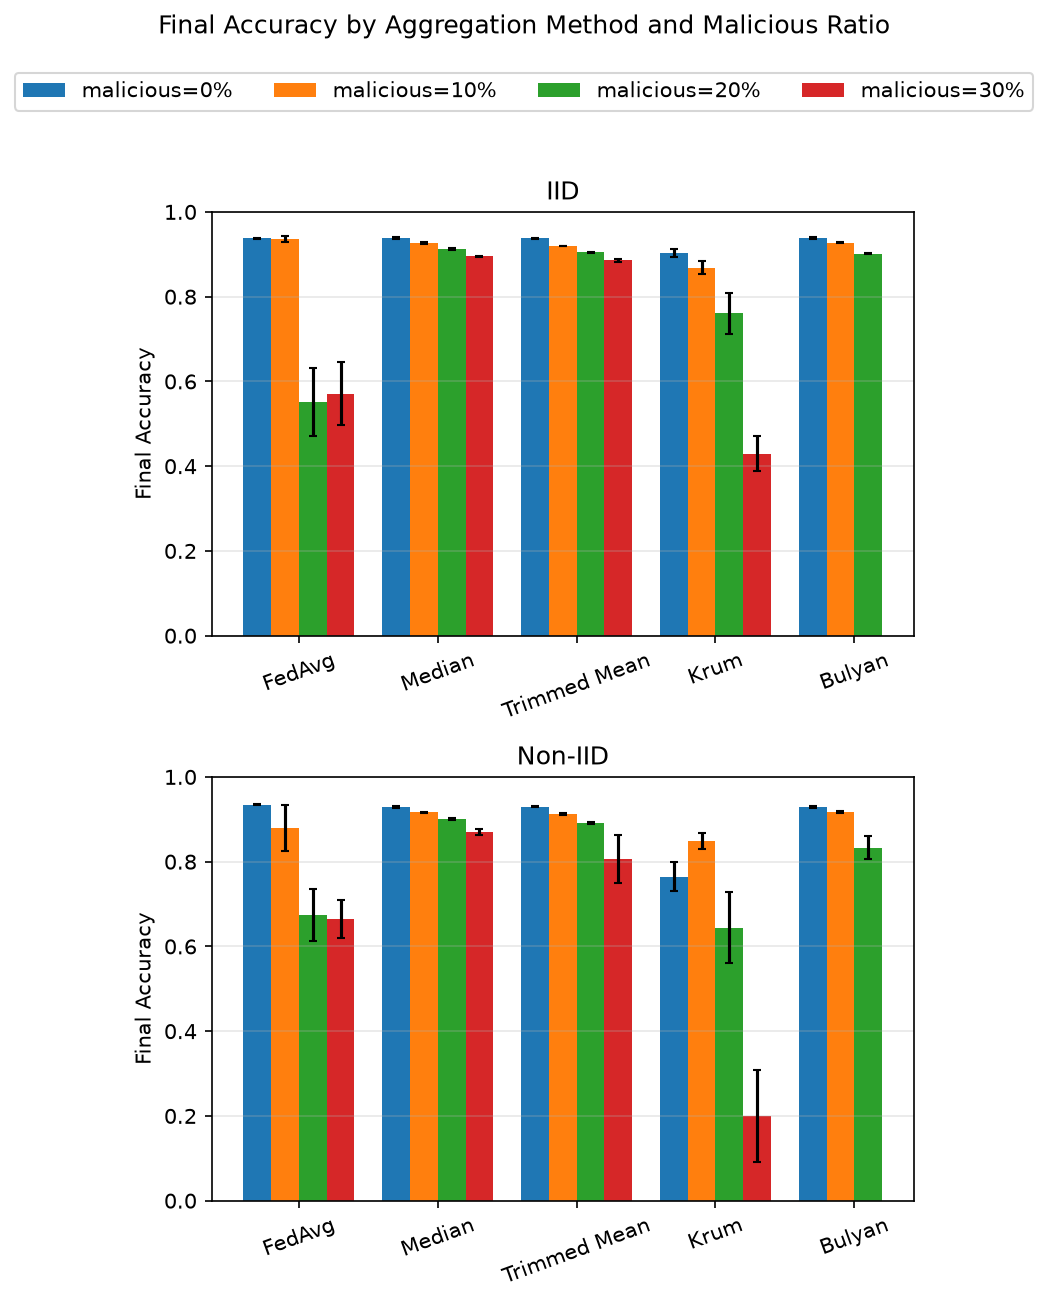
\includegraphics[width=\columnwidth]{summary_final_accuracy_bar.png}
    \caption{集約手法 × 悪性クライアント比率別の最終Accuracy（summary.csv，Seed平均±標準偏差）}
    \label{fig:summary_bar}
\end{figure}

\begin{figure}[H]
    \centering
    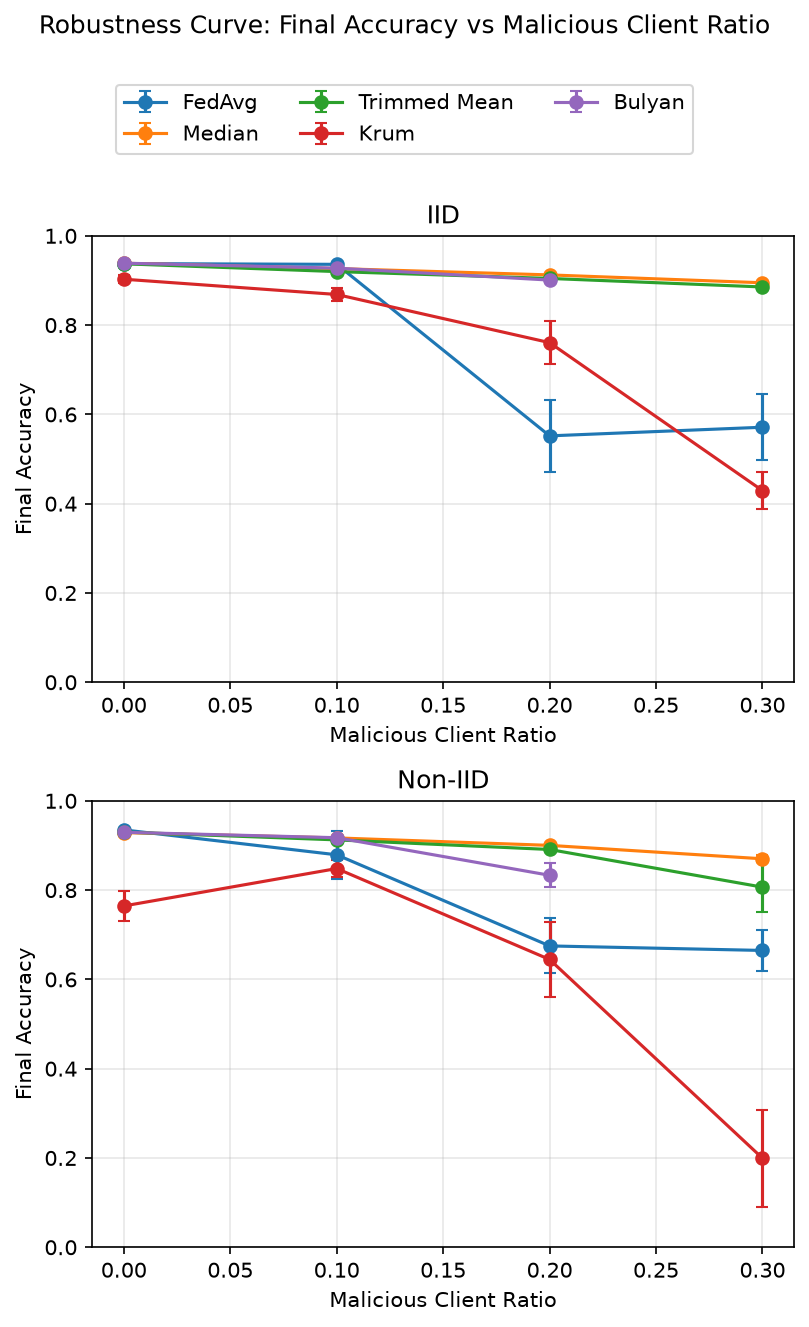
\includegraphics[width=\columnwidth]{summary_robustness_curve.png}
    \caption{悪性クライアント比率に対する頑健性曲線（summary.csv，Seed平均±標準偏差）}
    \label{fig:summary_robustness}
\end{figure}

\clearpage
\subsection{FedAvg：悪性クライアント比率 0.2 以上で急激に不安定化}

FedAvg（防御なし単純平均）は，悪性クライアント比率 0.1 までは
IID・Non-IID いずれの環境でも最終 Accuracy が約 0.94（IID）／
約 0.88--0.94（Non-IID）を維持し，Seed 間のばらつきも小さかった．
これは，100クライアント中最大10クライアントの悪性更新が
単純平均に混入しても，残り90\%の正常な更新によって
平均が大きく引き寄せられる希釈効果によるものと考えられる．

一方，悪性クライアント比率 0.2 以上では状況が一変し，
最終 Accuracy は IID で約 0.55（比率0.2）・0.57（比率0.3），
Non-IID で約 0.67（比率0.2）・0.66（比率0.3）まで低下した．
さらに Round ごとの Accuracy・Loss が大きく振動する不安定な挙動が
学習全体を通じて観測され（例：IID・比率0.3では Round 3 に
Loss が最大 16.05 に達する），Seed 間のばらつきも
標準偏差で 0.05--0.08 程度まで拡大した．
FedAvg は集約時に外れ値を除外する仕組みを持たないため，
悪性クライアントが送信する大きくスケールされた悪性更新
（真の更新量を10倍に拡大したもの）がそのまま単純平均に混入し，
グローバルモデルを毎ラウンド大きく振動させたと考えられる．
すなわち，希釈効果による頑健性は悪性クライアント比率が
一定の水準（本実験では10\%程度）を下回る場合にのみ有効であり，
それを超えると防御機構を持たない単純平均は Adaptive attack に対して
急激に脆弱になることが確認された．

\subsection{Median / Trimmed Mean / Bulyan：緩やかな性能劣化}

座標ごとの頑健統計量に基づく Median・Trimmed Mean，および Krumによる候補選定と
Trimmed Mean を組み合わせた Bulyan は，いずれも悪性クライアント比率の増加に伴って
最終 Accuracy が緩やかに低下する傾向を示した
（例：Median（IID）は比率0.0の約0.939から比率0.3で約0.895へ，
Trimmed Mean（IID）は約0.937から約0.885へ低下）．
学習曲線は全体として単調増加に近く，Krumのような急激な悪化や崩壊は見られなかった．
ただし Bulyan は Non-IID・比率0.2で最終Accuracyが約0.83まで低下するなど，
Non-IID 環境下でやや不安定さが増す傾向も観測された．
また Bulyan は理論的制約 $n \geq 4f+3$ により，
悪性クライアント比率0.3（$f=30$，$n=100$）では
$4f+3=123>100$ となり集約自体が破綻することが確認された．
これは攻撃への頑健性以前に，クライアント数と許容する悪性クライアント数の
比率設計そのものに制約があることを示しており，実運用上は
悪性クライアント比率の上限を事前に見積もった上で
クライアント数を十分に確保する必要があることを示唆する．

\subsection{Krum：Adaptive attack に対する構造的な脆弱性}

標準的な Krum（本実験では multi\_k=1）は，5手法の中で最も不安定な挙動を示した．
Krum は複数クライアントの更新を平均せず，Krumスコア（他クライアントとの距離の近さ）が
最小となる1クライアントの更新のみをそのまま次ラウンドの大域モデルとして採用する．
この設計は単一の悪性更新に対する頑健性を理論的に保証する一方で，
平均化によるノイズ低減効果を持たないため，選択される1クライアントが入れ替わるたびに
大域モデルが不連続に変化しやすいという弱点を持つ．

実際，Krum（IID，比率0.2以上）およびKrum（Non-IID，比率0.1以上）では，
学習中盤（おおむね Round 7--15 付近）まで Accuracy が上昇したのち，
終盤にかけて明確に低下する非単調な挙動が複数のSeedで観測された
（例：Krum（IID，比率0.3）は Round 7 付近の約0.76をピークに
Round 20 では約0.40--0.46まで低下）．
これは，Adaptive attack が過去ラウンドの大域モデルを観測しながら
悪性更新を作成する設計であるため，学習が進むにつれて
「統計的に多数派に近い」悪性更新を生成できるようになり，
Krumのスコアリングを回避して悪性クライアントの更新が選択される
頻度が高まったことを示唆している．
さらにKrum（Non-IID，比率0.3）では，Accuracyが Round 20 まで
0.12--0.28程度の低水準にとどまり，Lossも3.0--3.7まで発散するなど，
実質的に学習が崩壊した状態が確認された．
非IID性によってクライアントごとの局所分布が元々ばらついている状況では，
「1クライアントの更新のみを採用する」というKrumの性質そのものが
不安定性を増幅させたと考えられる．

\subsection{まとめ}

本実験の範囲では，頑健性の観点から
Median・Trimmed Mean（緩やかな劣化，安定した単調収束，
比率0.3でも最終Accuracy約0.87--0.90を維持）
$>$ Bulyan（比率0.2までは同水準に良好だが，理論的制約 $n \geq 4f+3$
により比率0.3では集約自体が破綻）
$>$ FedAvg／Krum（いずれも比率0.2以上で急激に不安定化・低下するが，
IID・Non-IIDで優劣が逆転する）
という傾向が確認された．
FedAvg と Krum はいずれも外れ値を除外する仕組み（Krumは単一クライアント
選択，FedAvgはそもそも除外機構を持たない）が Adaptive attack によって
実質的に無効化される点で共通するが，IID・比率0.3ではKrumがより低く
（最終Accuracy約0.43，FedAvgは約0.57），Non-IID・比率0.3では逆に
FedAvgがKrumを上回る（FedAvg約0.66，Krum約0.20）というように，
データ分布によって両者の相対的な脆弱性が入れ替わる点は興味深い．
特にKrumで観測された「学習中盤でのピーク後の性能低下」，および
FedAvgで観測された「悪性クライアント比率が希釈効果の限界を超えた
とたんに急激に不安定化する」という2つの現象はいずれも，
静的な攻撃（攻撃者が固定戦略を用いる場合）を前提とした頑健性保証や
希釈効果だけでは，Adaptive attackのような適応的な攻撃者に対して
不十分となりうることを示す実験的傍証として注目に値する．

\end{document}
